\documentclass{article}
\usepackage{array, booktabs, graphicx, apacite, setspace}
\usepackage[titletoc,toc,title]{appendix}
\usepackage[toc,section=section]{glossaries}
\usepackage{tocloft}
\usepackage{titlesec}
\usepackage{float} % for image flush right



% set section indentation
\setcounter{secnumdepth}{4}


% add space between paragraphs
\setlength{\parskip}{\baselineskip}


% format \paragraph{example} as a subsubsubsection
\titleformat{\paragraph}
{\normalfont\normalsize\bfseries}{\theparagraph}{1em}{}
\titlespacing*{\paragraph}
{0pt}{3.25ex plus 1ex minus .2ex}{1.5ex plus .2ex}


% automatically convert "" to ``''
\usepackage [autostyle, english = american]{csquotes}
\MakeOuterQuote{"}


% define list of equations
\newcommand{\listequationsname}{\Large{List of Equations}}
\newlistof{myequations}{equ}{\listequationsname}
\newcommand{\myequations}[1]{
   \addcontentsline{equ}{myequations}{\protect\numberline{\theequation}#1}
}
\setlength{\cftmyequationsnumwidth}{2.3em}
\setlength{\cftmyequationsindent}{1.5em}


% format appendix numbering
\renewcommand\appendix{\par
  \setcounter{section}{0}
  \setcounter{subsection}{0}
  \setcounter{figure}{0}
  \setcounter{table}{0}
  \renewcommand\thesection{Appendix \Alph{section}}
  \renewcommand\thefigure{\Alph{section}\arabic{figure}}
  \renewcommand\thetable{\Alph{section}\arabic{table}}
}


% -------- GLOSSARY ENTRIES -------- %
\makenoidxglossaries

\newglossaryentry{word}{
	name={Word},
	description={Definition of the word}
}


% renames "Contents" to "Table of Contents"
\renewcommand\contentsname{Table of Contents}

\begin{document}

% -------------------------------------- %
% ------------ FRONT MATTER ------------ %
% -------------------------------------- %

% -------- TITLE PAGE -------- %

\title{\huge ELEC 402 \\ \Large \medskip Introduction to VLSI Systems}
\author{Charles Clayton}
\date{\today}
\maketitle
`
\thispagestyle{empty}

\pagenumbering{roman}
\setcounter{page}{0}


% -------- TABLE OF CONTENTS/LISTS -------- %

\singlespacing			\pagebreak
\tableofcontents		\pagebreak

\listoffigures		
\listoftables
\listofmyequations
\pagebreak


% -------- GLOSSARY -------- %

\printnoidxglossaries	\pagebreak


% ----------------------------- %
% -------- MAIN MATTER -------- %
% ----------------------------- %

\pagenumbering{arabic}
\singlespacing

\section{Path to VLSI Systems}

In 2014, 250 billion \textit{billion} transistors were created. Every second, 8 trillion transistors were crated. That's 25 times the number of stars in the milky way, and 75 times the number of galaxies in the known university. VLSI systems originally meant between 20k-1M transistors, and beyond that was called ULSI for "ultra", but since the amount of transistors on a die accelerated so fast that new terminology would have to be constantly developed, we stuck with the VLSI terminology.

And he have arrived at this point in a very short period of time, only the last 50 years. The first electronic computer was the ENIAC in 1946, and this used entirely vacuum tubes. The first transistor was created in Bell Labs in 1948. The first integrated circuit was in 1958. The start of Moore's law was in the first microprocessor, the Intel 404 in 1971.

In the previous decades, increases in performance could be reliably gained by increasing the clock speed of processors and reducing the size of the transistors to fit more transistors an the same size die. However, by reducing the size there was no space for the heat to radiate, so the higher frequency and the smaller sizes reached the point where the power consumption was no longer worth the tradeoff. 

Since then, clock speeds have plateaued and we we must increase performance by implementing architectural changes and taking advantage of parallelism. There is currently a divide between software and hardware engineers, and the goal now is to find a way to bridge this gap, for instance by taking HDLs to a higher abstraction layer to make it more possible to be programmed like C.

Smaller transistors means improved performance, not only because you can have more transistors in the same amount of a space, but because smaller transistors have less capacitance so they consume less power have smaller latency.

We are reaching the end of Moore's law however. The size of atoms is a fundamental barrier. When a gate size gets too small there are a limited number of electrons available to us. When there were about 800 electrons, if one electron passes or doesn't pass through the transistor, that isn't a significant change in performance. However, when you can only fit 20 electrons to a transistor, any leakage or tunneling have significant effects on the performance. We are also reducing the voltage supply of circuits to consume less power, but this increases our changes of  exceeding the threshold voltage of transistors and accidentally turning them on.

\section{CMOS Manufacturing}

Silicon is the 2nd most abundant element in the earth's crust. It is a semiconductor, which allows it to be very flexible in its conductive properties when we take advantage of doping it with impurities. 

The difference between and MOSFET and a BJT is that a MOSFET, unlike a BJT, requires no current into the gate, which is better for digital systems and makes the mathematics more simple.

A FinFET behaves more similar to an ideal transistor and has less noise, lower threshold voltages, and better performance and lower power consumption. As a bonus, the math is the same for FinFETs and CMOS, so they are designer agnostic.

...


\section{Introduction to SystemVerilog}


\section{MOSFETs}

BJTs are not used it digital circuits because they require a gate  currents, whereas FETs switch very well without gate currents.

\subsection{PN Junctions}

Silicon has X valence electrons. P-type materials (an anode) are silicon doped with boron. Boron has X-1 valence electrons, so the boron impurities will steal an electron from neighbouring silicon atoms, opening up a hole in the semiconductor that is free to move. This excess hole makes some people think of the material as positively (hence P) changed -- however this is a slight misconception because there are equivalent numbers of protons and electrons, so by themseleves these materials are neutral.

Similarly, an N-type material (a cathode) is doped with arsenic, which has X+1 valence electrons. This creates an extra electron in the semiconductor that is free to move. 

A PN junction creates a diode, allowing current in only one direction. This junction creates a depletion region where the electrons in the N material fill in the holes in the P material. This makes the P material negatively charged, and the N material positively charged (???), so the N material repels current. 

A MOSFET is this diode with a terminal above it for a gate voltage that can be applied. When a positive voltage is applied to the diode, it creates a conductive channel that overcomes this. Allowing us to use the diode as a switch. 

\subsection{MOS Operating Modes}

Let's ignore the source and the drain terminals and just look at how the body and gate of the MOS transistor works. 

The top layer of the transistor is a good conductor called a gate. This is where we apply the voltage to control the transistor. These are usually made of polysilicon. Early transistors had them made of metal, and metal is making a comeback now, but we'll still going to think of it as poly. 

The bottom layer is the body, it is made of doped silicon. The body of the transistor is always grounded. In this example the body is a P-type, so the carriers in this case are holes because there are "missing" electrons -- meaning it's an nMOS transistor. More on that in the next section.

The middle layer is an insulator called the gate oxide. This is made of $\mathrm{SiO_2}$. This is a good insulator, so almost no current flows from the gate to the voltage.

Let's look at what happens when we apply different voltages to the gate.

\begin{enumerate}
\item \textbf{Negative voltage} -- The gate develops a negative charge, so so this makes extra positively charged holes accumulate at the bottom of the gate. This is called \textit{accumulation mode}. In the picture the holes are evenly distributed, but in reality they should be denser at the top of the body.

\begin{figure}[ht!]
\centering
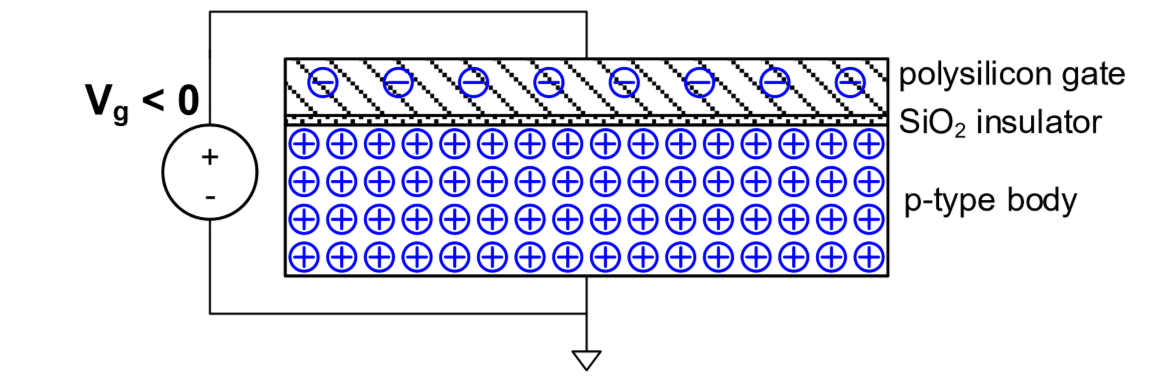
\includegraphics[width=70mm]{mos.png}
\caption{Accumulation of an nMOS}
\end{figure}

\item \textbf{Small voltage} -- If the applied voltage is positive but less than the threshold voltage, $V_t$, the holes in the body are repelled away from the gate. This creates a \textit{depletion} region beneath the gate.

\begin{figure}[ht!]
\centering
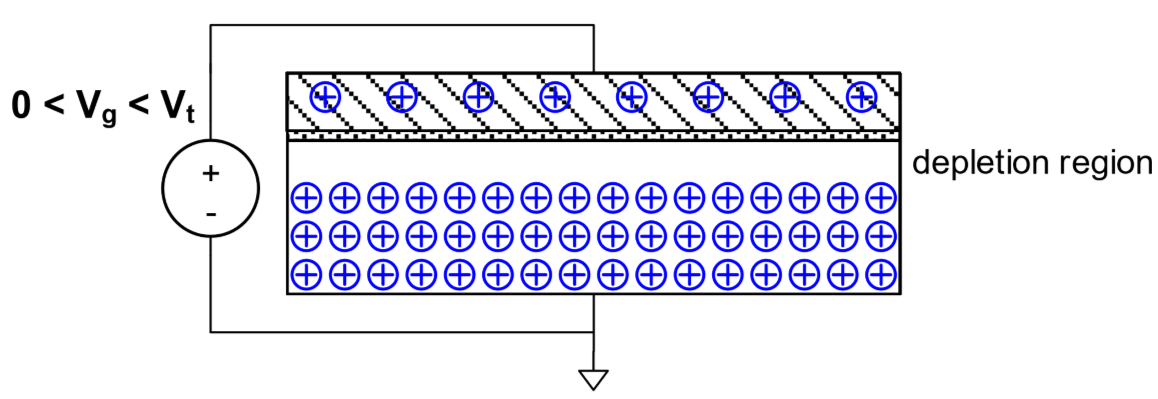
\includegraphics[width=70mm]{mos2.png}
\caption{Depletion of an nMOS}
\end{figure}


\item \textbf{Large voltage} -- If the applied voltage is greater than the threshold voltage then the holes are repelled even further to the bottom of the body, and some electrons move up to the gate. This creates a conductive band of free electrons called the \textit{inversion} layer.

\begin{figure}[ht!]
\centering
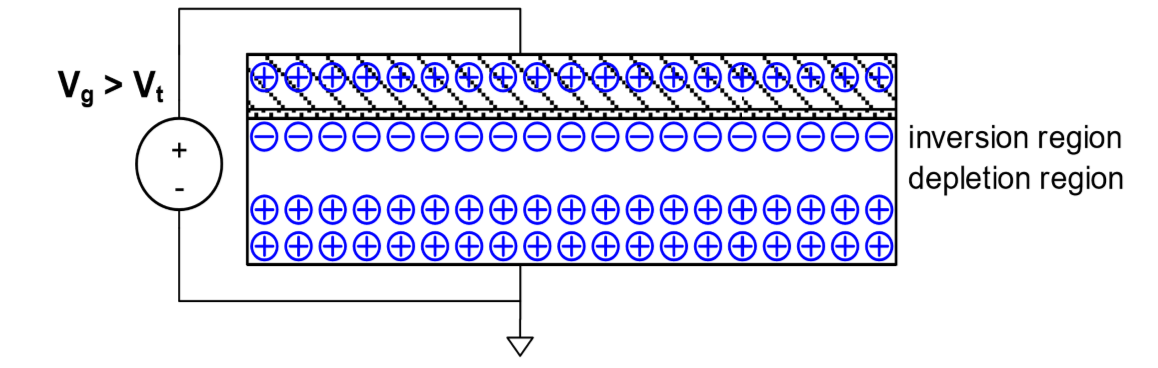
\includegraphics[width=70mm]{mos3.png}
\caption{Inversion of an nMOS}
\end{figure}

\end{enumerate}

In essence, this is how a transistor works. With a P-type body, if you apply a voltage and you open up conductive band which can carry current. With an N-type body, if you don't apply a voltage, you have a conductive band, if you do apply a voltage you can close the conductive band.


\subsection{nMOS Transistor}

A transistor is actually a four terminal device -- Gate, Source, Drain, and Body. Usually the body terminal is just connected to ground, so we often treat it as a three terminal device. 


\begin{figure}[ht!]
\centering
\includegraphics[width=60mm]{NMOS.png}
\caption{nMOS Transistor}
\end{figure}


MOS stands for Metal Oxide Semiconductor, and an nMOS means that both the source and drain terminals are N-type material. The gate-oxide-body stack acts like a capacitor. 

\subsubsection{MOSFET Modes of Operation}

The mode of operation depends on the values of the drain, gate, and source voltages.

\begin{equation}
\begin{matrix}
V_{gs} = V_g - V_s \\
V_{gd} = V_g - V_d \\
V_{ds} = V_d - V_s 
\end{matrix}
\end{equation}
\myequations{Terminal Voltages in MOSFET}

Physically, the source and drain are symmetrical terminals. By convention however, we can determine which is the drain and source because the source has a lower voltage, $V_s < V_d$, therefore $V_{ds} \ge 0$. This is an easy interview question -- they will ask you to label the terminals, the drain is whichever terminal has a higher voltage.

Logically, remember the source is the source of electrons, not current which goes in the opposite direction. So the current is flowing from the drain to the source, so of course the source would need a  lower voltage. You can often assume that the source  is 0V. 

\begin{enumerate}
\item \textbf{Cutoff} -- There is no current flowing from the drain to the source (except for some non-ideal leakage perhaps), $I_{ds} = 0$. In an nMOS this means the gate is at low voltage (opposite with pMOS).

The Shockley model states the transistor is in cutoff when $V_{gs}<V_{t}$.


Note that diodes should always be reverse-bias. Forward-biased diodes are bad because you will get static current, and you only want dynamic current to flow in a digital circuit. (???)

\item \textbf{ON} -- Current is allowed to flow from the drain to the source. In an nMOS, this means the gate is at high voltage. This creates a negatively changed (N-type) channel in the body under the gate through which current can flow. (???) While ON, the transistors could also be in Linear or Saturated mode.

\end{enumerate}

The supply voltage, $V_{dd}$ was 5V in the 1980s, but has decreased to 3.3V, 2.5V, 1.2V, and so on as transistors have gotten smaller. This is to prevent damaging tiny modern transistors and to save power. $V_{dd}$ is around 800mV for modern transistors.


\paragraph{Linear Mode}

Also called Resistive, in this mode of operation the current from the drain to the source $I_{ds}$, increases with $V_{ds}$. At this point, the transistor acts like a resistor. 

The Shockley model states the transistor is in linear when $V_{gs}>V_{t}$ (so that the transistor is on) and $V_{gd}>V_t$.


\begin{figure}[ht!]
\centering
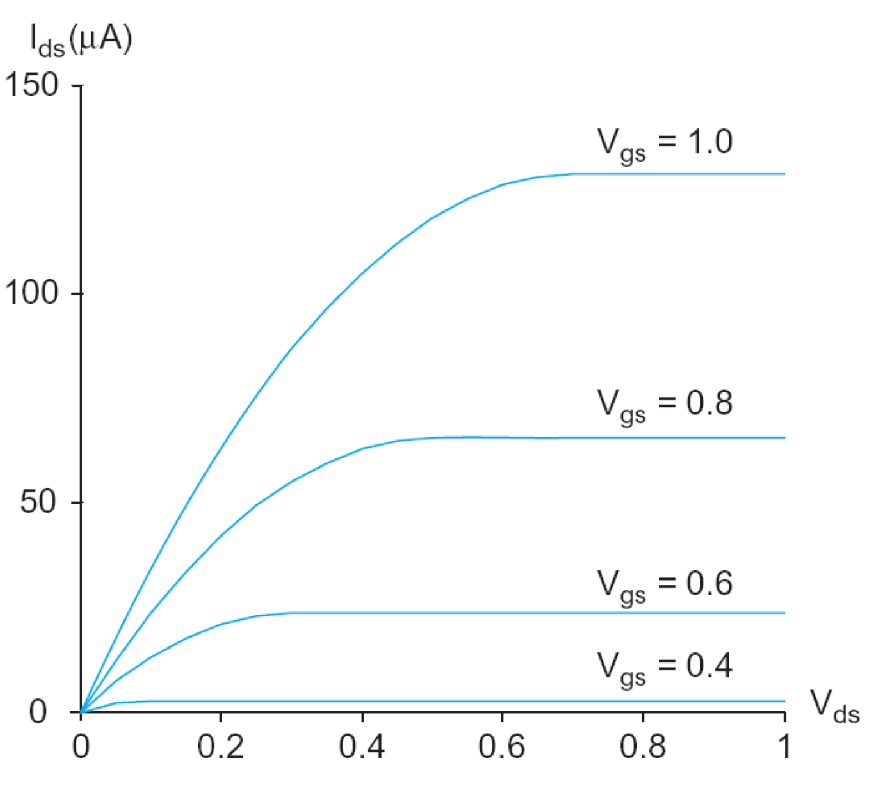
\includegraphics[width=60mm]{SquareLaw.png}
\caption{Shockley/Square-Law Model of a Real Transistor}
\end{figure}

When the transistor is in linear operation, our drain-to-source current is the following.

\begin{equation}
I_{ds} = \dfrac{\beta}{2}\left[ 2 ( V_{gs} - V_t ) - V_{ds} \right] V_{ds} = \beta \left( V_{gs} - V_{t}-\dfrac{V_{ds}}{2} \right) V_{ds}
\end{equation}
\myequations{Drain to source  current in linear}

In digital systems, since we can assume that $V_s$ is 0V, then $V_{gs} = V_{dd}$. We may also assume that $V_{ds}$ is small enough such that the resistance is linear, and $V_{ds}/2$ can be ignored.

To determine the resistance of a transistor, you can take the inverse of the slope of the $I_{ds}-V_{ds}$ curve. Note that at the origin the slope is steepest, so the resistance  is the least at the origin.

\begin{equation}
R_n = \dfrac{V_{ds}}{I_{ds}} = \dfrac{1}{\beta \left( V_{gs} - V_{t}-\dfrac{V_{ds}}{2} \right)}  \approx \frac{1}{\beta (V_{dd} - V_t)}
\end{equation}
\myequations{Resistance of nMOS in Linear Mode}



$\beta$ is the "transconductance coefficient" -- a constant based on the mobility of the carriers $\mu$, the oxide capacitance $C_{ox}$, and the length and width of the channel.

\begin{equation}
\beta = \mu C_{ox}\dfrac{W}{L} 
\end{equation}
\myequations{Transconductance coefficient, $\beta$}

\paragraph{Saturated}

In Saturation mode, $I_{ds}$ begins to reach a maximum and no longer increases linearly with $V_{ds}$. At this point, instead of acting like a resistor, the transistor acts like a current source.

\begin{equation}
I_{ds} = \dfrac{\beta}{2} (V_{gs} - V_t)^2
\end{equation}
\myequations{Drain-source current in saturation}

The Shockley model states the transistor is in saturation when $V_{gs}>V_{t}$ (so the transistor is on) and $V_{gd}<V_{t}$.

\subsubsection{Shockley Model}

\begin{equation}
\begin{matrix}
V_{gs}<V_{t} & \rightarrow & Cutoff \\
V_{gs}>V_{t} & \rightarrow & On \\
\\
V_{gd}>V_t & \rightarrow & Linear \\
V_{gd}<V_t & \rightarrow & Saturation
\end{matrix}
\end{equation}
\myequations{Shockley Model of nMOS transistor}

\subsubsection{Designing Actual Transistors}

You can play around with the width of the transistor, increasing the width reduces the resistance of the transistor but takes up more space. However, the length of the resistor should be constant because you want the transistor to be fast, we will use a reasonable value of 45nm.

70 degrees Celsius is the nominal voltage of most digital design, and the threshold voltage of an nMOS is 300mV. In our model, $\mu C_{ox} = 262$ so $\beta = 262 \times W/L$.

\subsection{pMOS Transistor}

A pMOS is very similar to the nMOS transistor with some key differences. The gate and the drain having P-type doping, so instead of providing the gate with a voltage to turn the transistor on, you provide the gate with zero voltages.

In digital design, this is represented with a bubble at the gate of the transistor. In analog design, nMOS versus pMOS is indicated by the direction the arrow is pointing in. 

\begin{figure}[ht!]
\centering
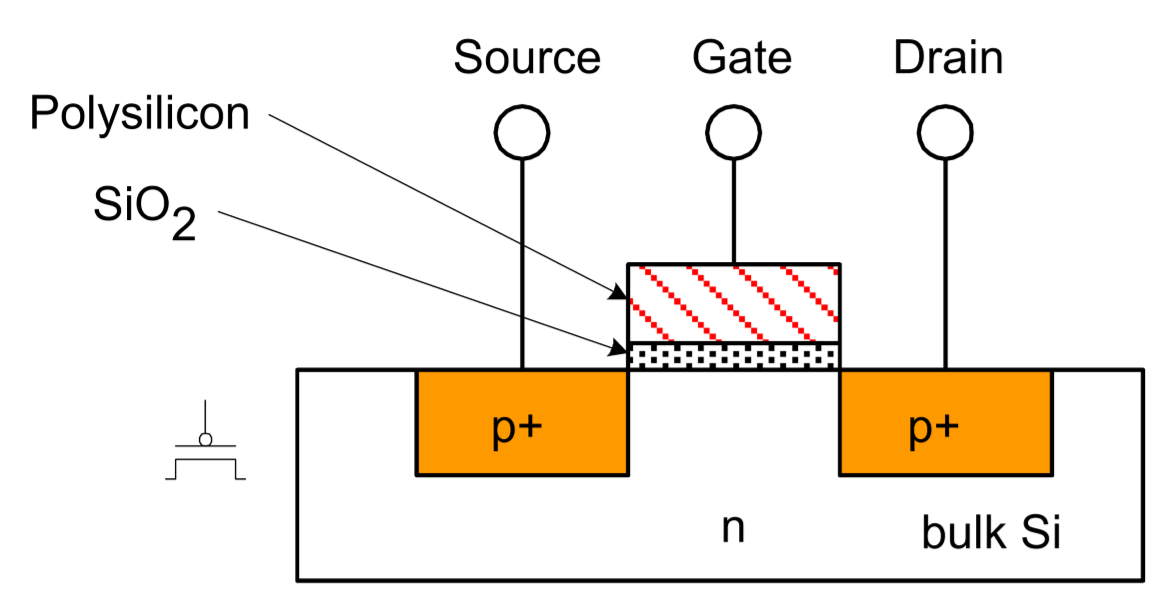
\includegraphics[width=60mm]{pMOS.png}
\caption{pMOS Transistor}
\end{figure}


Intuitively, the nMOS seems better to work with because the logic is 1--on, 0--off. But in terms of design, the main difference between the pMOS and the nMOS is that the nMOS is fast at transferring a 0 signal, whereas the pMOS is fast at transferring a 1 signal.

Additionally, for strange physics reasons, the mobility of holes as carriers is 2x  lower than the mobility of electrons as carriers. This is because the holes have a higher effective mass than electrons, even though they're just empty space where an electron goes. So that's weird, but  we will use $\mu_n/\mu_p = 2$.

This means that a pMOS which has to transfer holes has worse performance. To compensate for this, pMOS transistors are usually 2x as wide.

When analyzing pMOS transistors, it is easier to disregard sign and remember the same rules as the nMOS transistor but with swapped subtraction, and using the absolute value of the threshold voltage.

\begin{equation}
\begin{matrix}
V_{sg}< |V_{t}| & \rightarrow & Cutoff \\
V_{sg}> |V_{t}| & \rightarrow & On \\
\\
V_{dg}> |V_t| & \rightarrow & Linear \\
V_{dg}< |V_t| & \rightarrow & Saturation
\end{matrix}
\end{equation}
\myequations{Shockley Model of pMOS transistor}

\subsection{MOS Capacitance}

Any two conductors separated by a dielectric have some capacitance.

The reason digital systems consume power is because when capacitances are charged, they discharge to ground.

If a transistor is small, your capacitance is smaller. If your capacitance is smaller, you can run faster and you use less power, so capacitance is very important.

\subsubsection{Diffusion Capacitance}

The gate oxide overlaps with the drain and the source somewhat with a distance of $X_d$. The effective length is the length of the gate minus the overlap.

\begin{figure}[ht!]
\centering
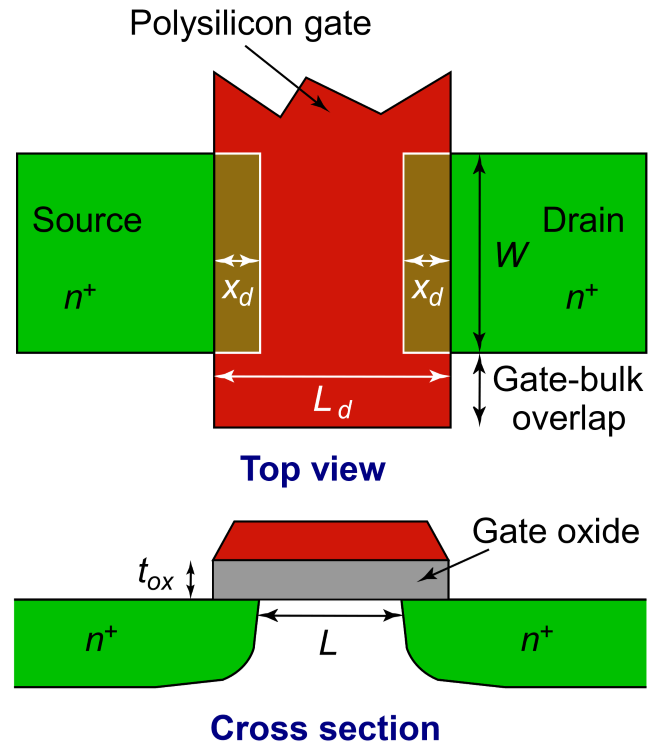
\includegraphics[width=60mm]{Length.png}
\caption{Effective Length}
\end{figure}


$$L_e = L_d - 2 X_d$$

This overlap creates the diffusion capacitance. This is a parasitic capacitance between the source and the body, and the drain and the body, $C_{sb}$ and $C_{db}$.

When you merge contacts between transistors you can reduce this diffusion capacitance.

\begin{figure}[ht!]
\centering
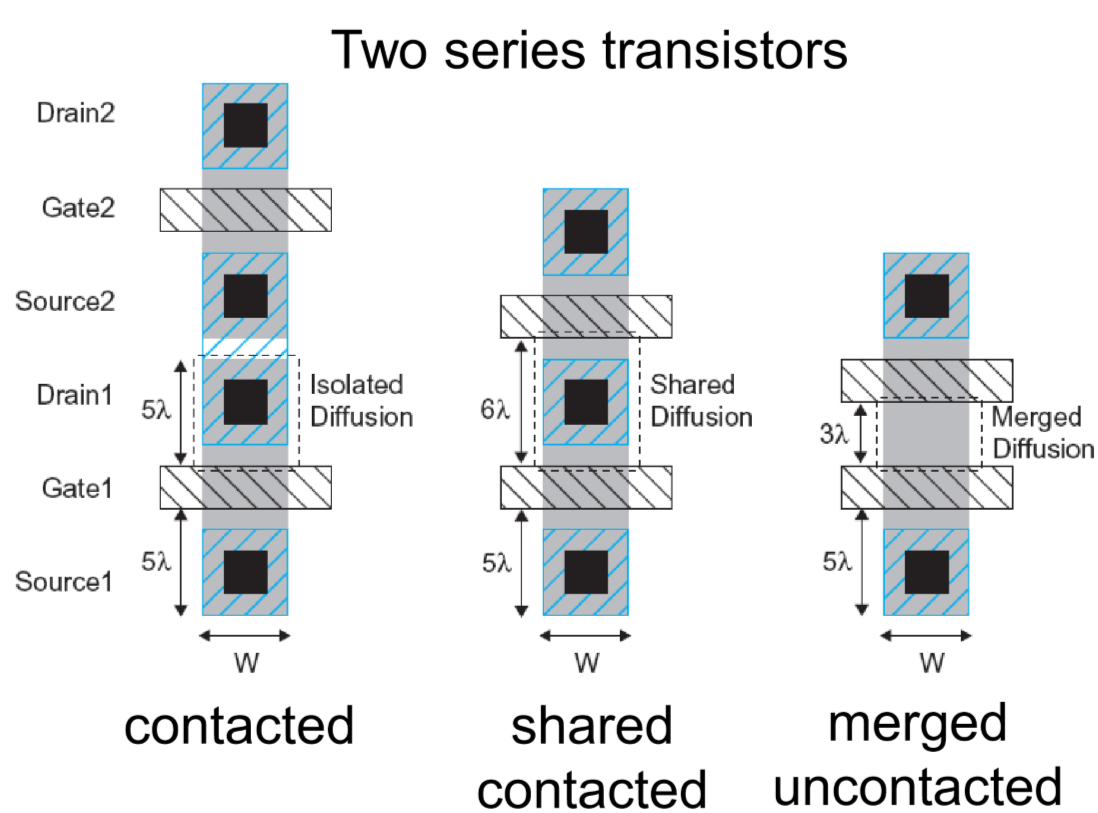
\includegraphics[width=80mm]{Diffusion.png}
\caption{Merged Transistor Diffusions}
\end{figure}


\subsubsection{Gate Capacitance}

The gate capacitance $C_g$, is the sum of the capacitance between the gate and the body, the gate and the source, and the gate of the drain of the transistor. It is not constant, but varies depending on the mode of the transistor.

\begin{equation}
C_g = C_{gb} + C_{gs} + C_{gd}
\end{equation}
\myequations{Gate capacitance}

\begin{enumerate}
\item \textbf{Cutoff}, $V_g < 0$ -- The gate-to-body capacitance is at a maximum $C_0$, but there is no gate-to-source or gate-to-drain capacitance. So capacitance is approximately equal to $C_0$.

\item \textbf{Linear}, $0 < V_g < V_t$ -- The gate-to-body capacitance drops to zero. The channel charge is shared between gate-to-source and gate-to-drain capacitance, so both are $C_0/2$ and total capacitance is $C_0$.

\item \textbf{Saturation}, $V_{gs} > V_t$ -- The gate-to-body capacitance is zero, and beyond $V_t$ the $C_{gs}$ goes to $2C_0/3$.
\end{enumerate}


\begin{figure}[ht!]
\centering
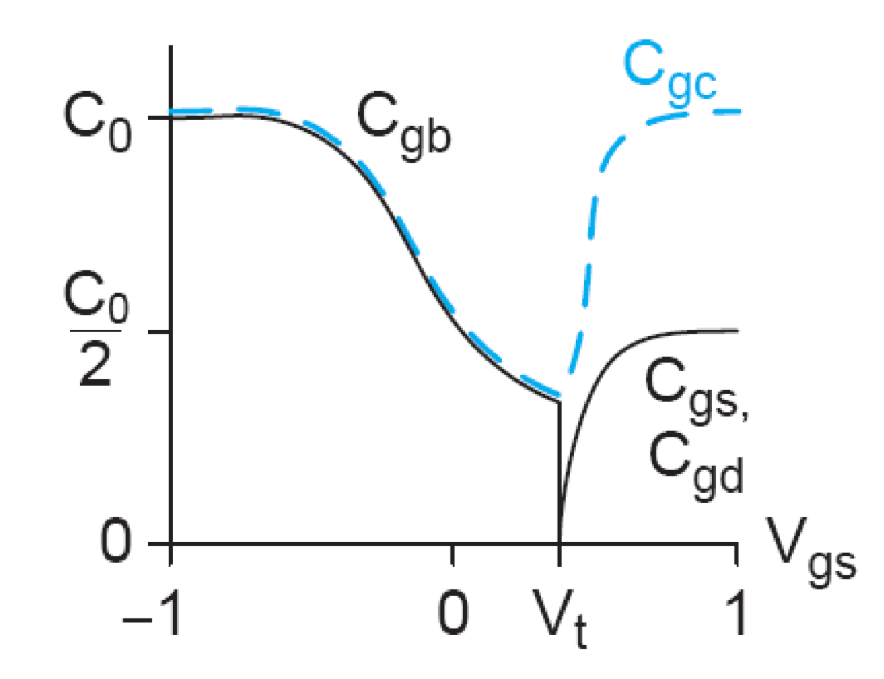
\includegraphics[width=60mm]{GateCapacitance.png}
\caption{Gate Capacitance}
\end{figure}


The gate capacitance is the same whether the transistor is in linear or saturated. However it drops when in saturation.

\begin{table}
\centering
\begin{tabular}{cccc}
\toprule
 & \textbf{Cutoff} & \textbf{Linear} & \textbf{Saturation} \\
 \midrule
 $\ \ \ C_{gb}$ & $C_0$ & 0 & 0 \\ 
 $\ \ \  C_{gs}$ & $0$ & $C_0/2$ & $2C_0/3$ \\ 
  $+\ C_{gd}$ & $0$ & $C_0/2$ & 0 \\ 
 \midrule
  $\ \ \ C_{g}$ & $C_0$ & $C_0$ & $2C_0/3$ \\ 
  \toprule

\end{tabular}
\caption{Gate Capacitance in Different Modes}
\end{table}

Capacitance can also be signal-dependent. If you have a capacitance of 1pF, you can apply a signal in such a way that the capacitance disappears. 

If you apply an in-phase signal to both sides of the capacitor, you short the signal by putting the same voltage on both sides, so there is no capacitance/impedance between them.

If you apply out-of-phase signals to both sides, then you apply twice the voltage difference and double the capacitance. So send signals in phase to minimize capacitance.

Let's look at some cases.

\newpage

\begin{figure}[ht!]
\centering
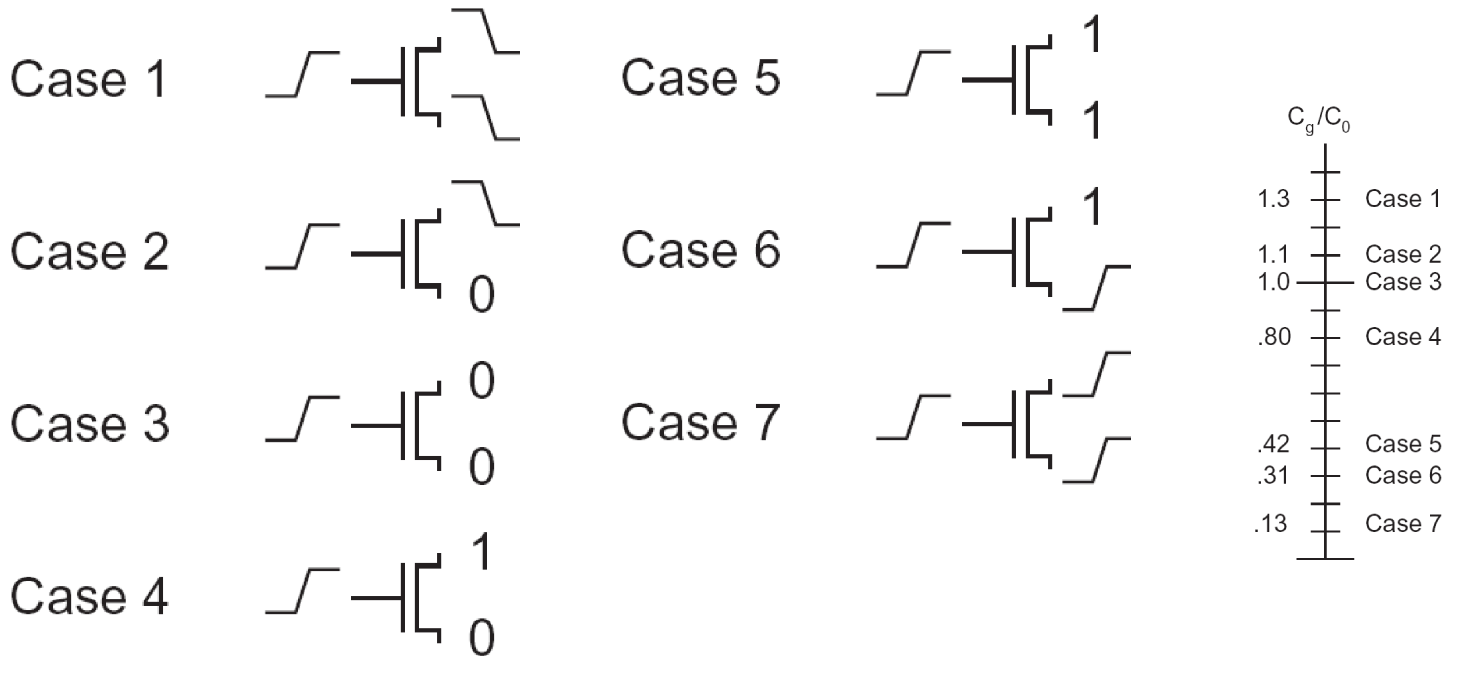
\includegraphics[width=100mm]{Signals.png}
\end{figure}

\small
\begin{enumerate}

\item \textbf{Case 1} \begin{itemize}
\item \textit{Initial} -- $V_{gs} = 0 - 1 < V_t \rightarrow$ OFF

\item \textit{Final} -- $V_{gs} = 1 - 0 > V_t$, $V_{gd} = 1 - 0 > V_t \rightarrow$ LINEAR

\item All signals out of phase, so $C_g$ a bit higher than $C_0$
\end{itemize}

\item \textbf{Case 2} \begin{itemize}
\item \textit{Initial} -- $V_{gs} = 0 < V_t \rightarrow$ OFF

\item \textit{Final} -- $V_{gs} = 1 > V_t$, $V_{gd} = 1 > V_t \rightarrow$ LINEAR

\item One signal out of phase, so $C_g$ a tiny bit higher than $C_0$
\end{itemize}

\item \textbf{Case 3} \begin{itemize}
\item \textit{Initial} -- $V_{gs} = 0 < V_t \rightarrow$ OFF

\item \textit{Final} -- $V_{gs} = 1 > V_t$, $V_{gd} = 1 > V_t \rightarrow$ LINEAR

\item $C_g$ is equal to $C_0$, some capacitance between G and S, and G and D 
\end{itemize}

\item \textbf{Case 4} \begin{itemize}
\item \textit{Initial} -- $V_{gs} = 0 < V_t \rightarrow$ OFF
\item \textit{Final} -- $V_{gs} = 1 > V_t$, $V_{gd} = 0 \rightarrow$ SATURATED
\item Some capacitance between G and S, $C_g = 2C_0/3$
\end{itemize}

\item \textbf{Case 5} \begin{itemize}
\item \textit{Initial} -- $V_{gs} = -1 < V_t \rightarrow$ OFF
\item \textit{Final} -- $V_{gs} = 0 < V_t \rightarrow$ OFF 
\item All voltages are the same so capacitance is slightly less than $C_0$
\end{itemize}

\item \textbf{Case 6} \begin{itemize}
\item \textit{Initial} -- $V_{gs} = 0 < V_t \rightarrow$ OFF
\item \textit{Final} -- $V_{gs} = 0 < V_t \rightarrow$ OFF 
\item G and S moved together, so slightly less capacitance than case 5
\end{itemize}


\item \textbf{Case 7} \begin{itemize}
\item \textit{Initial} -- $V_{gs} = 0 < V_t \rightarrow$ OFF
\item \textit{Final} -- $V_{gs} = 0 < V_t \rightarrow$ OFF 
\item G and D, and G and S moved together, so even less capacitive than case 6
\end{itemize}

\end{enumerate}

\newpage
\normalsize

When delivering two side-by-side rails with out-of-phase clocks. You will have 2C capacitance between them. However, this can be improved by sending a ground rail between them. 

The voltage difference will be less between the clock and the ground, but the ground will also be closer so you will still end up with 2C between each clock and the ground. But since the two 2C are in parallel, your total capacitance will be reduced to 1C. 

When you have clocks, they make noise for the rest of the circuit, so in general its a good idea to put grounds on both sides to shield it. You can also have a three-way clock with each 120 degrees out of phase, so they cancel.

\section{Pass Gate}

An inverter is just a pMOS on top and an nMOS on the bottom. The pMOS is on top because it is good at transmitting a 1, so it can move the voltage from the Vdd rail to the output quickly and without much loss. The nMOS is on the bottom because it is good at transmitting a 0, so it can move the ground voltage to the output quickly.

\begin{figure}[ht!]
\centering
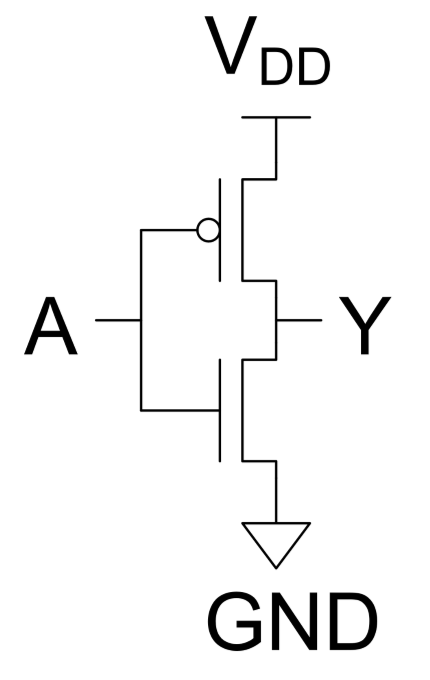
\includegraphics[width=20mm]{Inverter.png}
\caption{CMOS Inverter}
\end{figure}

If the pMOS and nMOS were swapped, it would be a buffer -- the output the same as the input. Except, in reality it would be slightly worse.

When the nMOS tries to transmit $V_{dd}$, it can't do it very well and only transmits $V_{dd} - V_{t}$. So for an input of 1V, it would only transmit about 700mV. 

When the pMOS tries to transmit GND, it can't do it very well either and instead of propagating 0V, it would transmit about 300mV. So our signal becomes less clear and strong overall.

Let's look at why this is. 

\subsection{nMOS Pass Gate}

Let's say we have our transistor in Figure 8 and we turn it on at $t=0$. Recall that the $V_s < V_d$, so the terminal on the right is the drain.  

\begin{figure}[ht!]
\centering
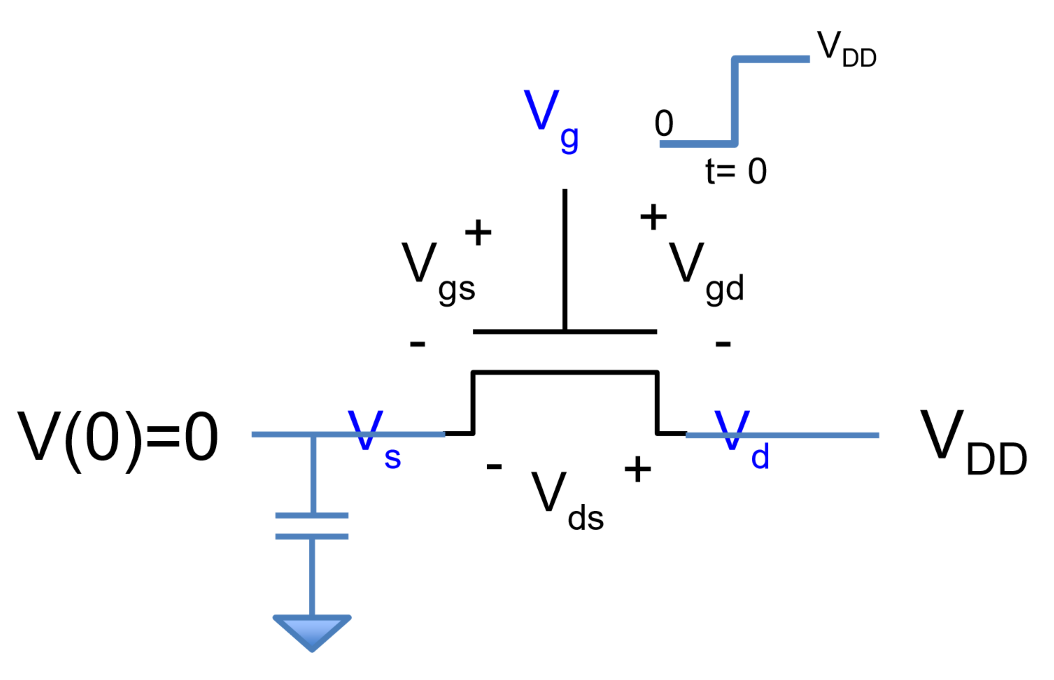
\includegraphics[width=60mm]{nPass.png}
\caption{nMOS Pass Filter (Vdd)}
\end{figure}

The current $I_{ds}$ will begin to flow from the drain to the source and charge up the capacitor at the source. As the capacitor charges exponentially fast, $V_{s}$ will increase and $V_{gs}$ will decrease. 

This means that transistor will eventually turn off when $V_s = V_{OH}$ (ie. $V_{gs} < V_t$), before it has completely charged the capacitor (the output) to $V_{dd}$. The highest output the nMOS can propagate is $V_{OH}$, roughly 700mV.

When the nMOS is transferring a 0V signal from the source to the drain, it's a different story. The voltage in the drain is free to discharge completely until $V_{gs} = V_{dd}$. The lowest output the nMOS can propagate is $V_{OL}$.

\begin{equation}
\begin{matrix}
V_{OH} = V_{dd} - V_{t}   \\ 
V_{OL} = 0 
\end{matrix}
\end{equation}
\myequations{Pass Gate of nMOS}

\begin{figure}[ht!]
\centering
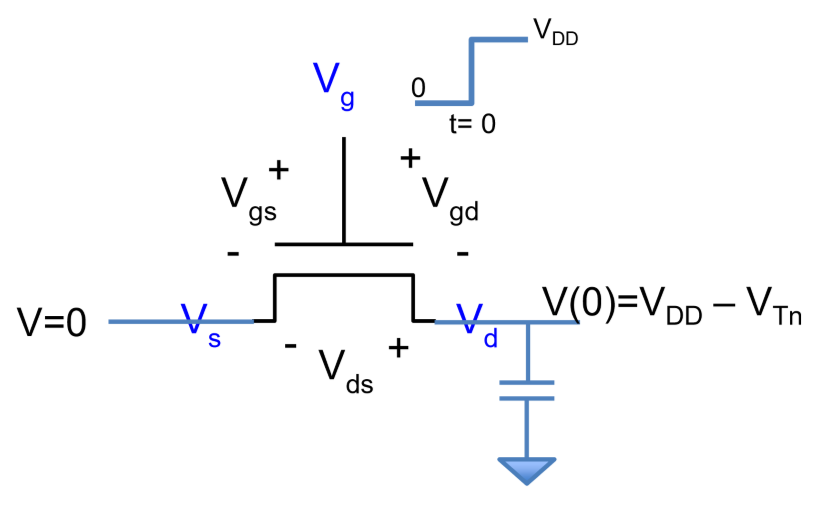
\includegraphics[width=60mm]{nPass1.png}
\caption{nMOS Pass Filter (0V)}
\end{figure}

\subsection{pMOS Pass Gate}

The explanation for this is the same as that of the nMOS, except reserved. The pMOS cannot properly transfer a 0V signal because it will turn off before the capacitor has completely discharged. Leaving a value of roughly 300mV as its output.Further, it will turn off slowly, throttling the charging so it happens sluggishly.

On the otherhand, it is good  at transferring a $V_{dd}$ signal and charges exponentially fast. This is why we connect $V_{dd}$ to a pMOS and GND to the nMOS. 

\begin{equation}
\begin{matrix}
V_{OH} = V_{dd}   \\ 
V_{OL} = V_{t}
\end{matrix}
\end{equation}
\myequations{Pass Gate of nMOS}

\section{Inverter}

Digital logic is all about highs and lows. You want nice clean and clear signals. If the voltage is somewhere in between, it's unclear what it is supposed to and you'll get bad behaviour. 

For instance, recall our inverter. If the voltage is for example around 500mV, both transistors may turn on and both may be in saturation. In this case, we would get a circuit flowing straight from $V_{dd}$ to GND, dumping all of our battery's charge.

\begin{figure}[ht!]
\centering
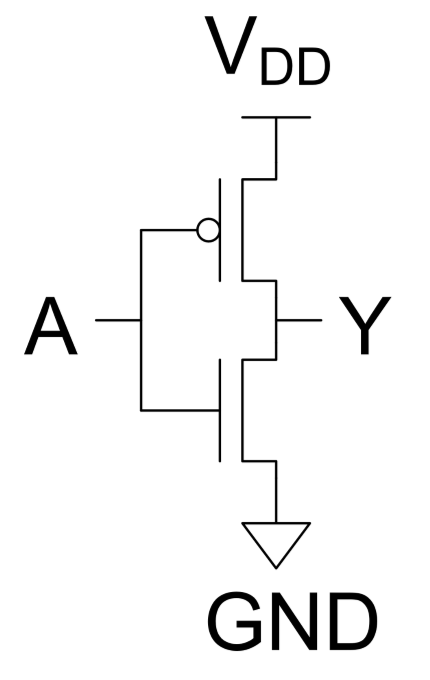
\includegraphics[width=28mm]{Inverter.png}
\end{figure}

\subsection{Operating Regions}

In reality, when the voltage A is switched, there is a temporary instance where both transistors are switching and current is momentarily allowed to flow. This is part of where our power dissipation comes from.  


\begin{figure}[ht!]
\centering
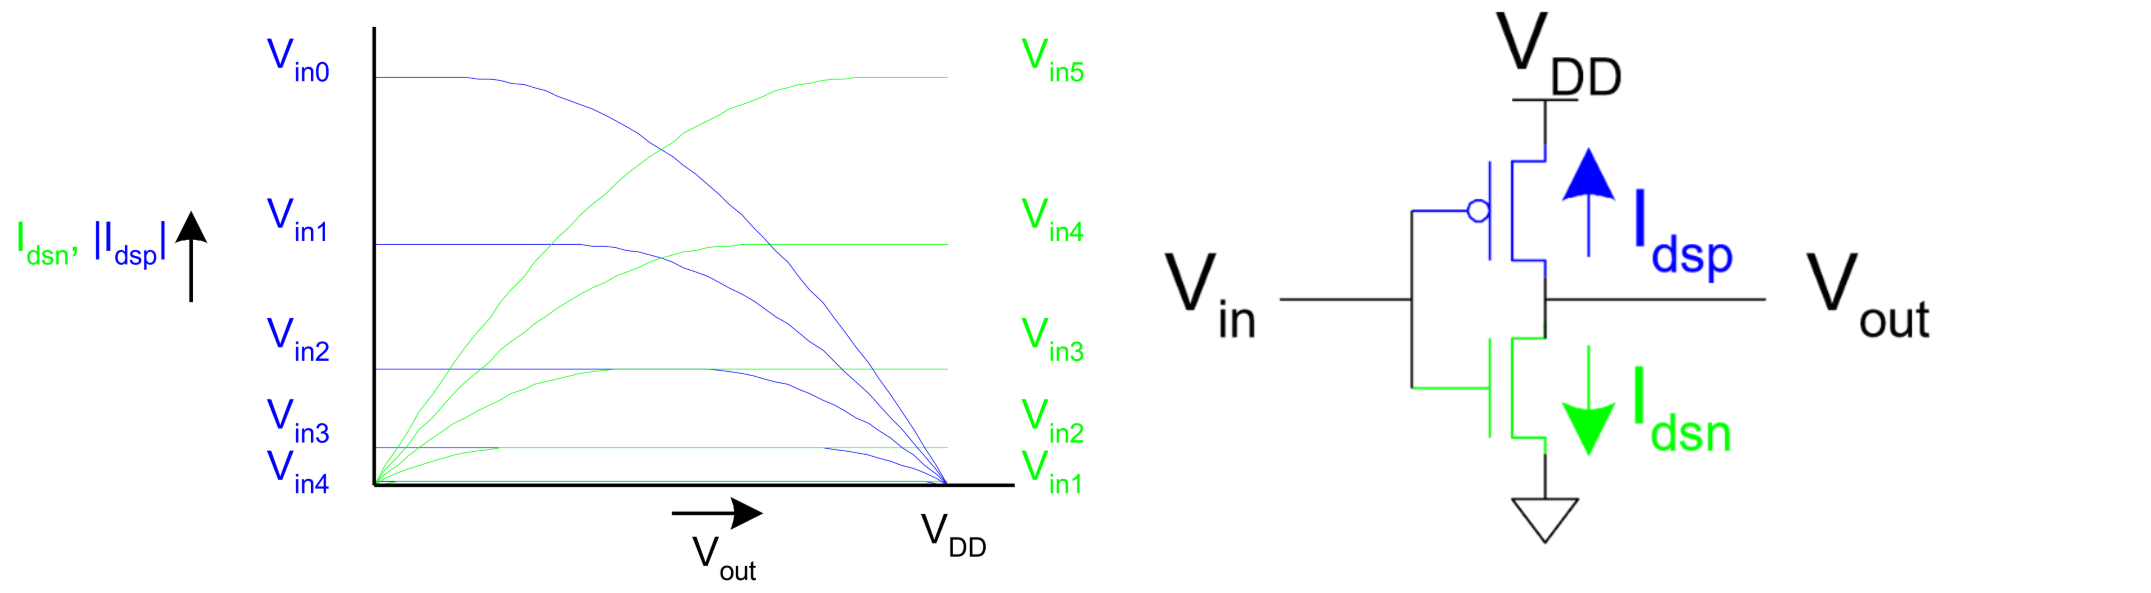
\includegraphics[width=130mm]{InverterIV.png}
\caption{IV Curve for pMOS (blue) and nMOS (green)}
\end{figure}

If we plot our output voltage vs. currents in the transistors, we can see the overlap of the current in the pMOS and nMOS. Our $V_{out}$ must be at a point where the currents are equal.  (???)

When we plot these values we can see the operating regions of the inverter. 

\begin{figure}[ht!]
\centering
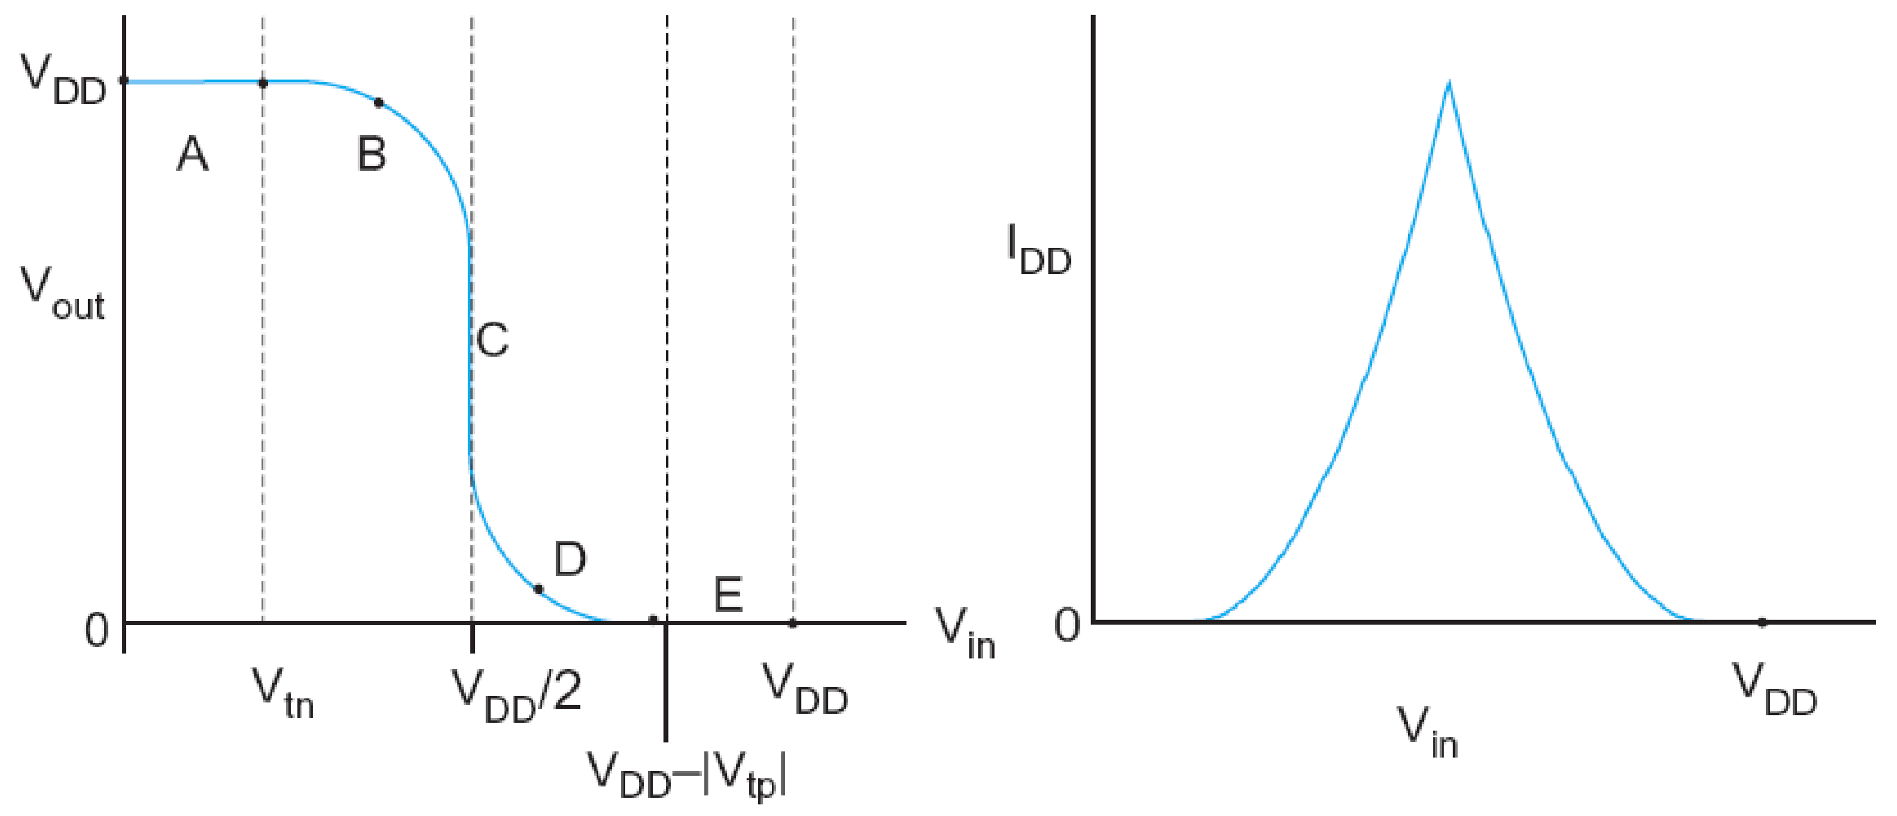
\includegraphics[width=90mm]{IV.png}
\caption{IV Curve for pMOS (blue) and nMOS (green)}
\end{figure}

As little time as possible should be spent in region C in Figure 11, because current is freely flowing from our supply to ground. The sharper the edges of our transistors, the less amount of current will be lost.

\begin{table}[ht!]
\centering
\begin{tabular}{lllll}
\toprule
\textbf{Condition} & \textbf{Region} & \textbf{nMOS} & \textbf{pMOS} & $\mathbf{V_{out}}$ \\
\midrule
$V_{in}<V_{t}$ & A & Cutoff & Linear & $V_{dd}$ \\
$V_t < V_{in} < V_{dd}/2$ & B & Saturated & Linear & $>V_{dd}/2$ \\
$V_{in} = V_{dd}/2$ & C & Saturated & Saturated & -- \\
$V_{dd}/2 < V_{in} < V_{dd} - V_t$  & D & Linear & Saturated & $<V_{dd}/2$ \\
$V_{dd} - V_t < V_{in}$ & E & Linear & Cutoff & 0 \\
\toprule
\end{tabular}
\caption{Operating Regions of an Inverter}
\end{table}

\subsection{Beta Ratio}

The point at which an inverter toggles is the $V_{inv}$. For an equally skewed inverter, when $\beta_p/\beta_n = 1$, the $V_{inv} = V_{dd}/2$. 

It's preferable to have a uniform skew, and usually we assume $\beta_p = \beta_n$. However, in a HI-skew the pMOS is stronger so $\beta_p > \beta_n$. Conversely, in a LO-skew the nMOS is stronger so $\beta_n > \beta_p$.

\begin{figure}[ht!]
\centering
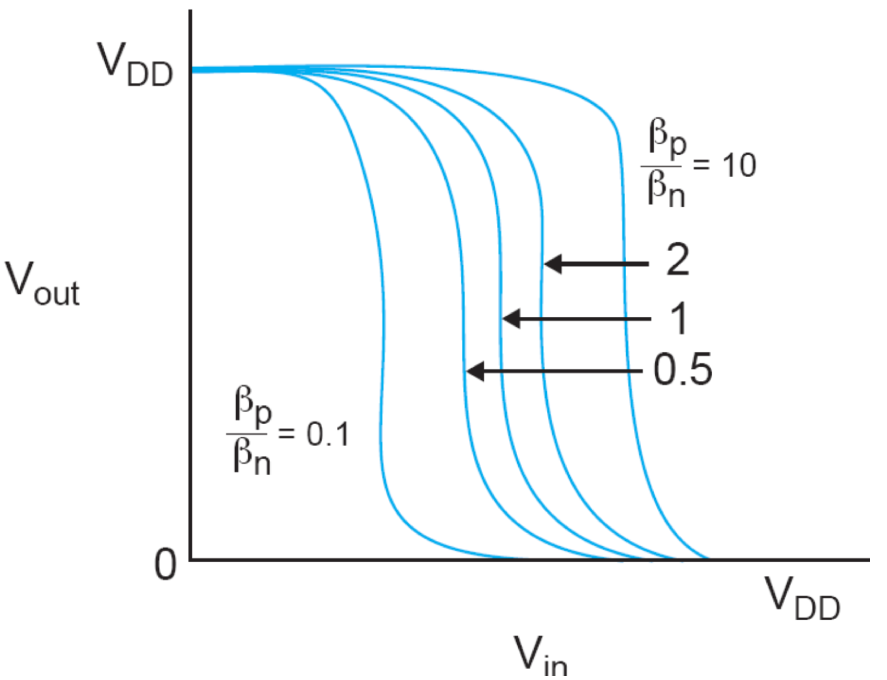
\includegraphics[width=50mm]{skew.png}
\caption{Beta Ratio/Skew}
\end{figure}

If your circuit is somehow biased to more easily charge than discharge, you may want to LO-skew it so that the discharging/charging is even.

\subsection{Noise Margins}

Here we look at how much noise a gate input can receive before it can't resolve the input. If your gate cannot recognize the input as one or a zero, then you are violating the noise margin of the system.

\begin{table}[ht!]
\centering
\begin{tabular}{lll}
\toprule
\textbf{Description} & \textbf{Symbol} & \textbf{Something} \\
\midrule
Minimum recognized high input & $V_{IH}$ & -- \\
Maximum recognized low input & $V_{IL}$ & -- \\
Minimum valid high output & $V_{OH}$ & -- \\
Minimum valid low output & $V_{OL}$ & -- \\
\toprule
\end{tabular}
\end{table}

\begin{equation}
\begin{matrix}
NM_L = V_{IL} - V_{OL} \\
NM_H = V_{OH} - V_{IH} \\
\end{matrix}
\end{equation}
\myequations{Noise Margins}

The noise margin is the difference between the worst case input and the worst case output. It is best to have $V_{IH}$ as close as possible to $V_{IL}$ to give yourself the largest possible noise margins so that all values can be resolved. 

\begin{figure}[ht!]
\centering
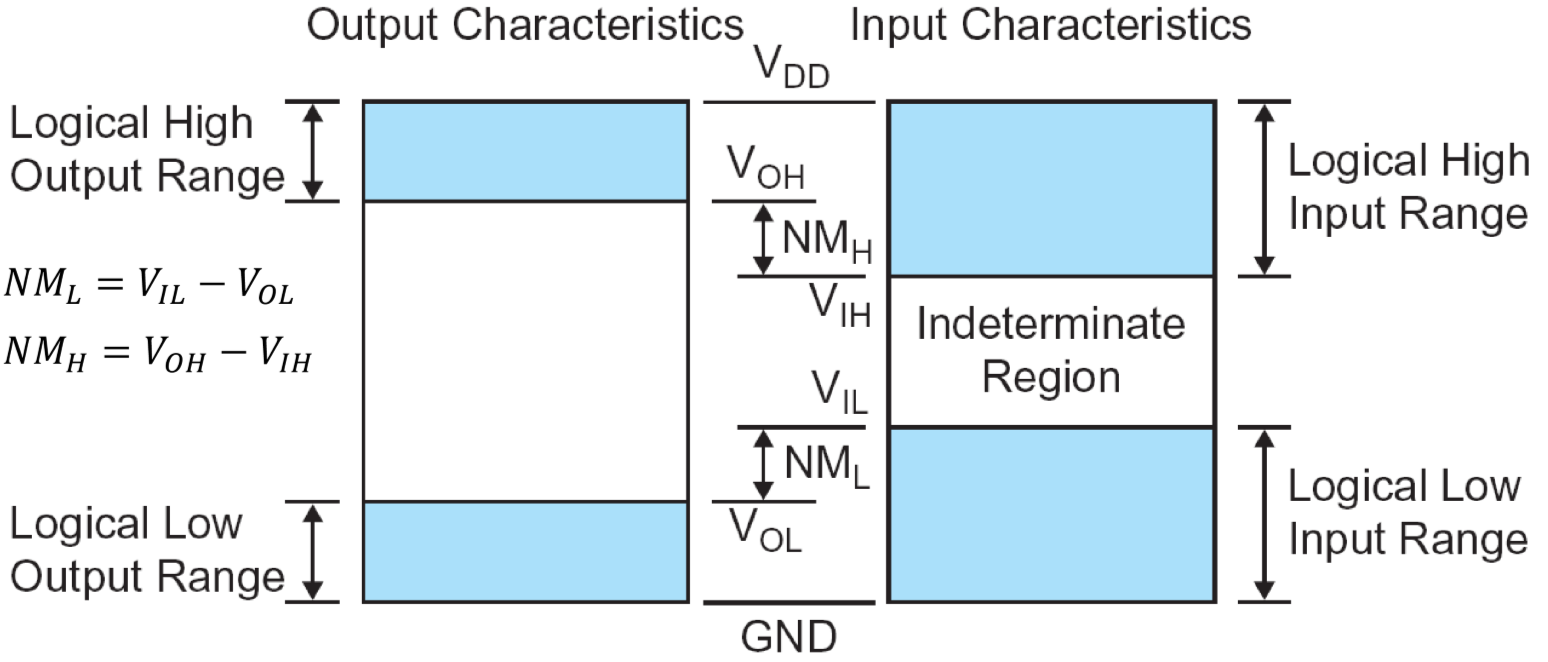
\includegraphics[width=90mm]{NM.png}
\caption{High and Low Noise Margins}
\end{figure}

To maximize noise margins, select the value of $V_{OH}$ as the value of $V_{out}$ at the point where the slope of the $V_{out}/V_{in}$ curve first drops to 1. Select $V_{OL}$ as the $V_{out}$ where the $V_{out}/V_{in}$ increases back up to one. 

\begin{figure}[ht!]
\centering
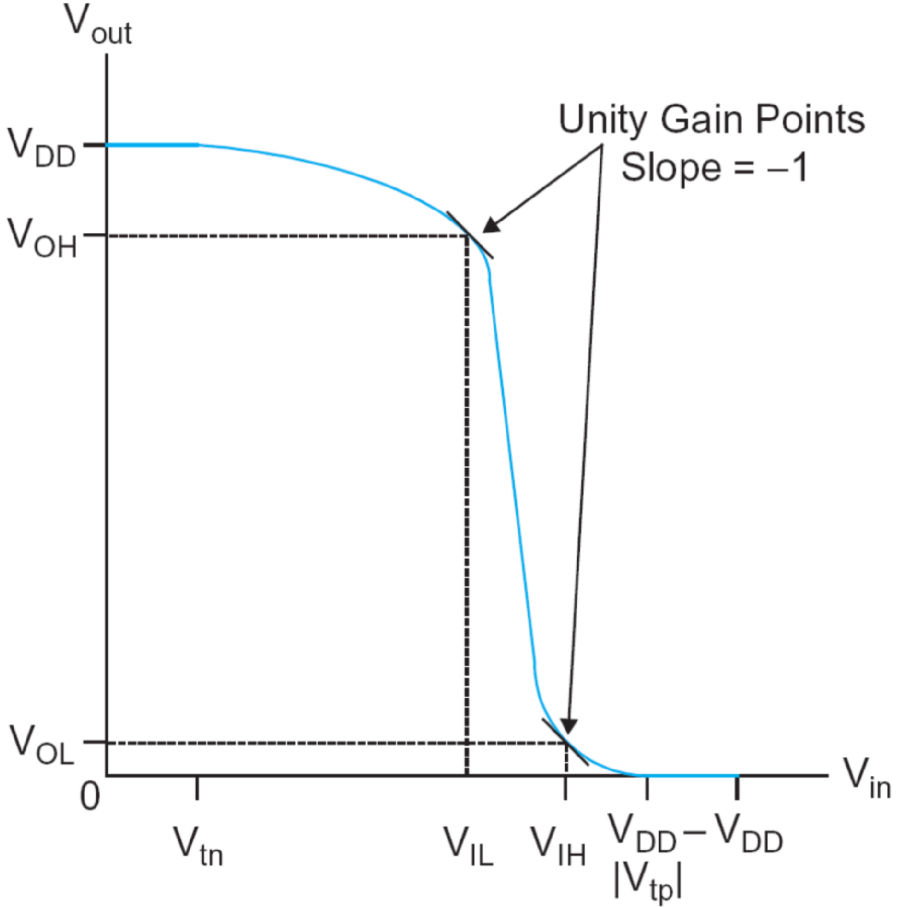
\includegraphics[width=50mm]{NoiseMargin.png}
\caption{Points of VOH and VOL from the DC transfer characteristic}
\end{figure}

\subsection{Inverter Delay}

When we talk about delay, we are usually talking about the propagation delay, $t_{pd}$ for either the rise or the fall time. 

The rise or fall propagation delay is defined as the \textit{maximum} time between the input crossing the 50\% point between high-and-low to the output crossing the 50\% point.

\begin{figure}[ht!]
\centering
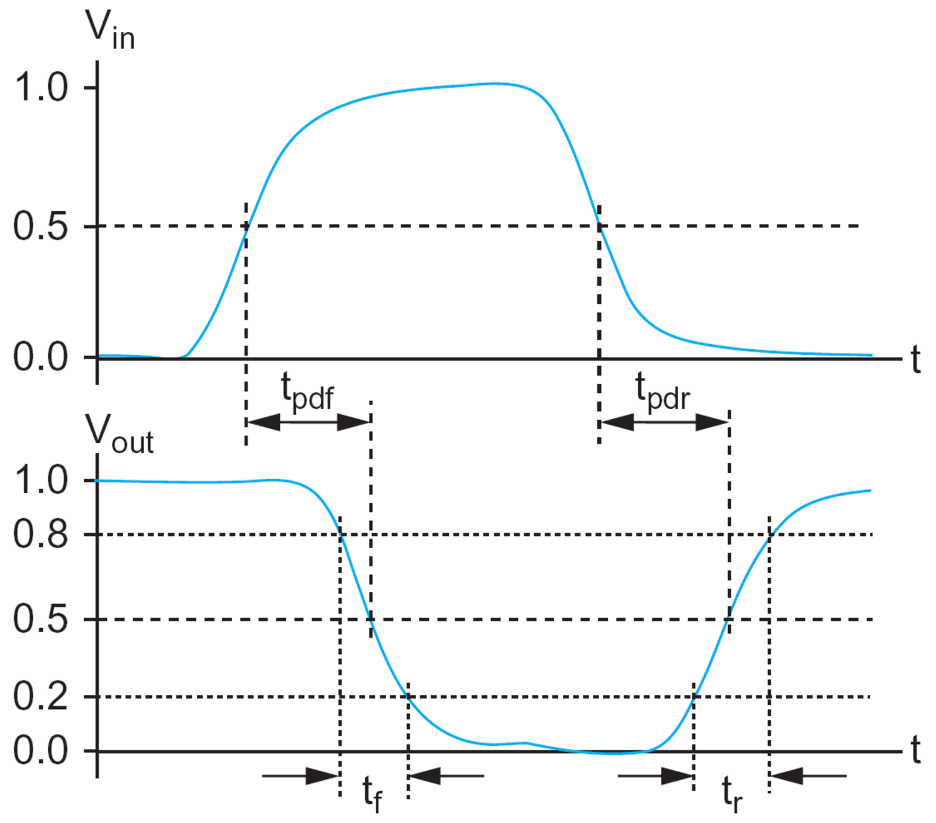
\includegraphics[width=60mm]{Delay.png}
\caption{Measurements of Inverter Delay}
\end{figure}

Propagation delay is usually taken as the average of the rise and fall propagation delays. It can also be approximated with an RC model.

\begin{equation}
t_{pd} = \dfrac{t_{pdr} + t_{pdf}}{2} \approx RC\mathrm{ln}(2)
\end{equation}

The contamination delay is the \textit{minimum} time from the input crossing the 50\% mark to the to the output crossing the 50\% mark.

We also may talk about the rise/fall times $t_r$ and $t_f$, which are the time taken to rise/fall from 10\% to 90\%. The average of these is the edge rate.

\section{Static CMOS Logic}

A combinational circuit is a circuit for which the output is a function only of the inputs -- such as just combinational logic like AND and OR gates. A sequential circuit is a function of the state of the circuit, or of previous inputs -- this requires some form of memory like latches. 

A static circuit always has a boolean output connected to either $V_{dd}$ or GND through a low-resistive path. It differs from a dynamic circuit in that it has no memory or storage of values to make use of at a later time, for instance in capacitors.

This is implemented through a complementary pull-up network (PUN) and pull-down network (PDN). The PUN is connected to $V_{dd}$ and is made up of only pMOS transistors. The PDN is connected to GND and only made up of nMOS transistors. 

\begin{figure}[ht!]
\centering
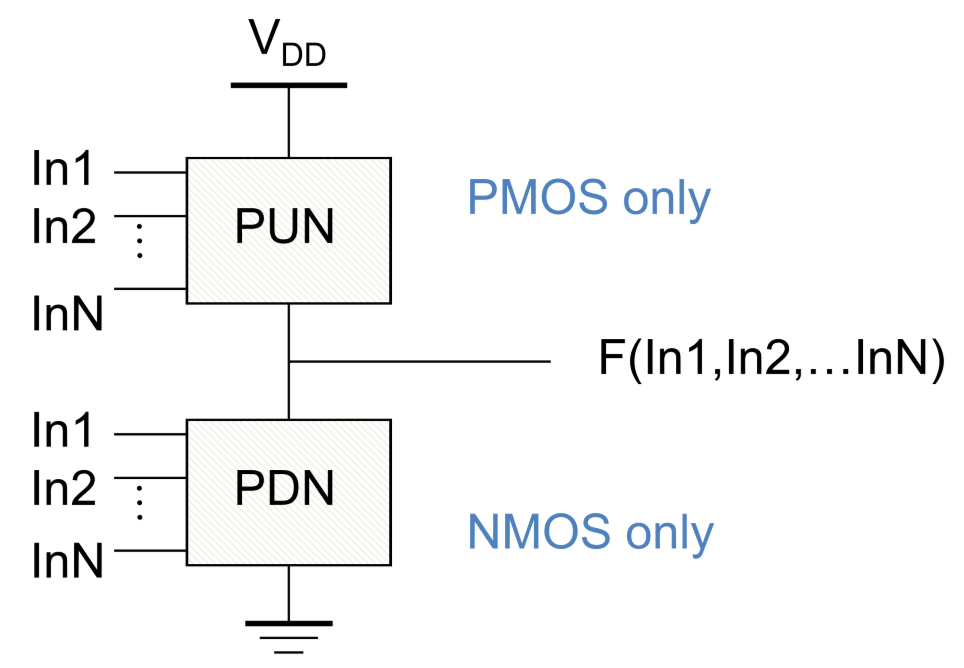
\includegraphics[width=60mm]{CMOS.png}
\caption{CMOS PUN and PDN}
\end{figure}

The inputs to the circuit go both toward the PUN and PDN. 

To implement combinational logic with our transistors, we can use two nMOS in series to act as an AND gate, and two pMOS in parallel to act as an OR gate. Recall that these will pass a strong 0 signal, but a weak 1 signal.

Similarly, we can implement a NAND gate with two pMOS in parallel, and a NOR gate with two pMOS in series. Again, these are good at passing a 1, but poor at passing a 0. 

To achieve a combinational logic that is both good at propagating a 1 and a 0, we use complementary PUN and PDN. 

For example, to implement a CMOS NAND gate, we first create an AND connection of nMOSs in the PDN. We then connect this to a NAND connection of pMOS in the PUN. The connection point is our output.

\begin{figure}[ht!]
\centering
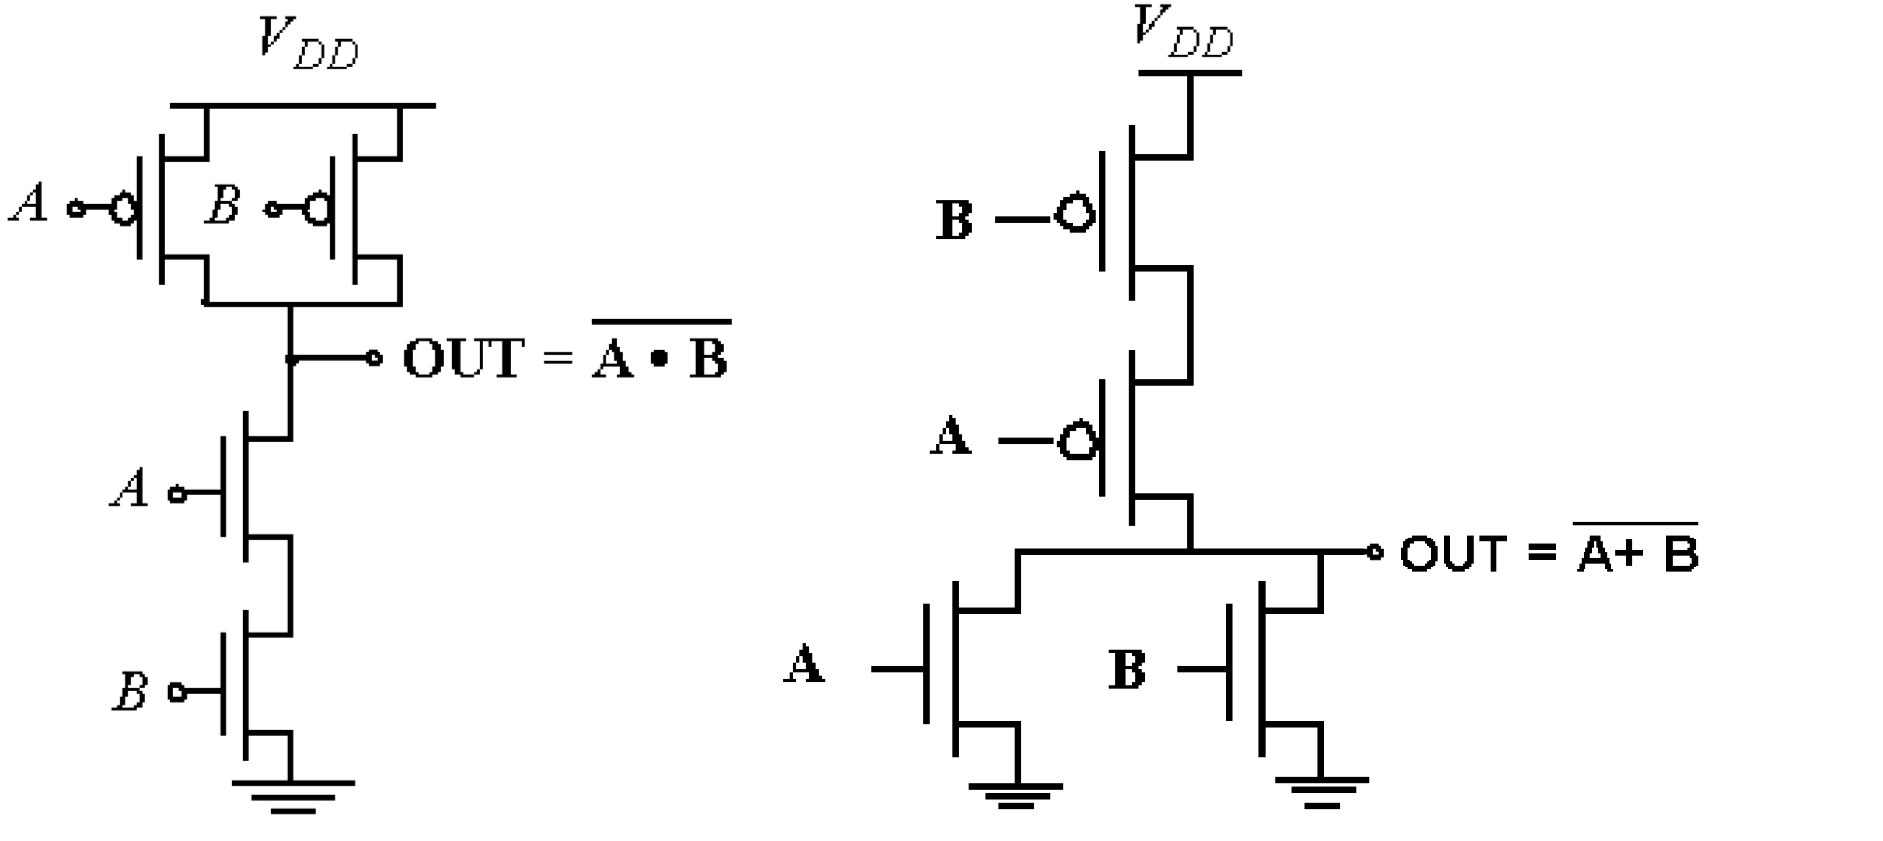
\includegraphics[width=100mm]{NAND2.png}
\caption{CMOS NAND2 Gate (Left) and NOR2 Gate (Right)}
\end{figure}

When designing these circuits, it's best to break it up in the following steps.

\begin{enumerate}
\item Take the complement of what you want to build -- the CMOS circuit outputs an inverted value

\item Design the nMOS PDN with the inverted logic. nMOS's are more intuitive -- series is AND, parallel is OR

\item Design the pMOS PUN by taking the complement of the nMOS network -- series becomes parallel and parallel becomes series
\end{enumerate}

By designing it this way, the output is always connected to $V_{dd}$ or GND, and pMOS is only transferring 1s and the nMOS is only transferring 0s.

There is also never contention -- a circumstance in which the output is both being driven from $V_{dd}$ and GND, which would consume power and output a confusing value.

\subsection{Preferred Capacitor Placement}

An additional consideration for these circuits is that if possible you want any single series transistors connected to the output, not the GND or $V_{dd}$, as indicated in Figure 17.

\begin{figure}[ht!]
\centering
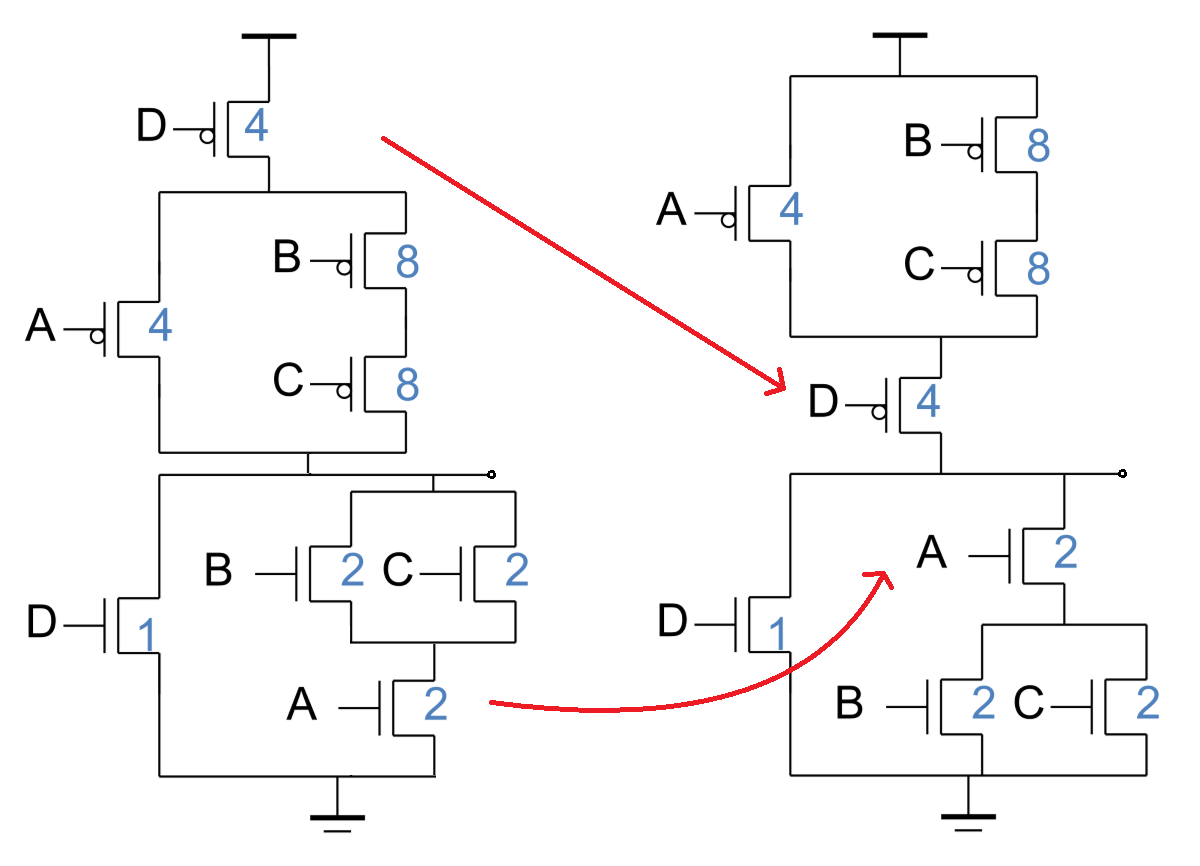
\includegraphics[width=80mm]{Capacitors.png}
\caption{Less Capacitance on the Output Rail (Right) is Better}
\end{figure}

In this case on the left, it simply means that there is more capacitance to charge on the output when switching between high and low. We want less output capacitance to increase the speed at which we can switch, so the case on the right is better. 


\subsection{Sizing for Equal Rise/Fall Timing}

We want the same delay in the PDN and PUN networks, so that the fall time and the rise time is even.

To do this, we have to make the equivalent resistance of each network the same.  We also want equal resistances through each path through the individual networks. This is achieved by modifying the size of the transistors.

The resistance is inversely proportional to the width.  Recall that by default the pMOS transistors are twice as large as the nMOS. 

Assume a capacitor is at the output of the CMOS circuit, and follow the output to the GND for each route through the PDN. Each of these routes should add up to $R_n$. So set the resistances of each transistor to some fraction of $R_n$ such that every route adds to $R_n$. The sizing for these transistors is then the inverse of that fraction. 

For the PUN, follow this same procedure. But recall that the pMOS are half as fast as the nMOS, so they must be sized to be twice as large from the start, so multiply the final value for size by 2. 


\begin{figure}[ht!]
\centering
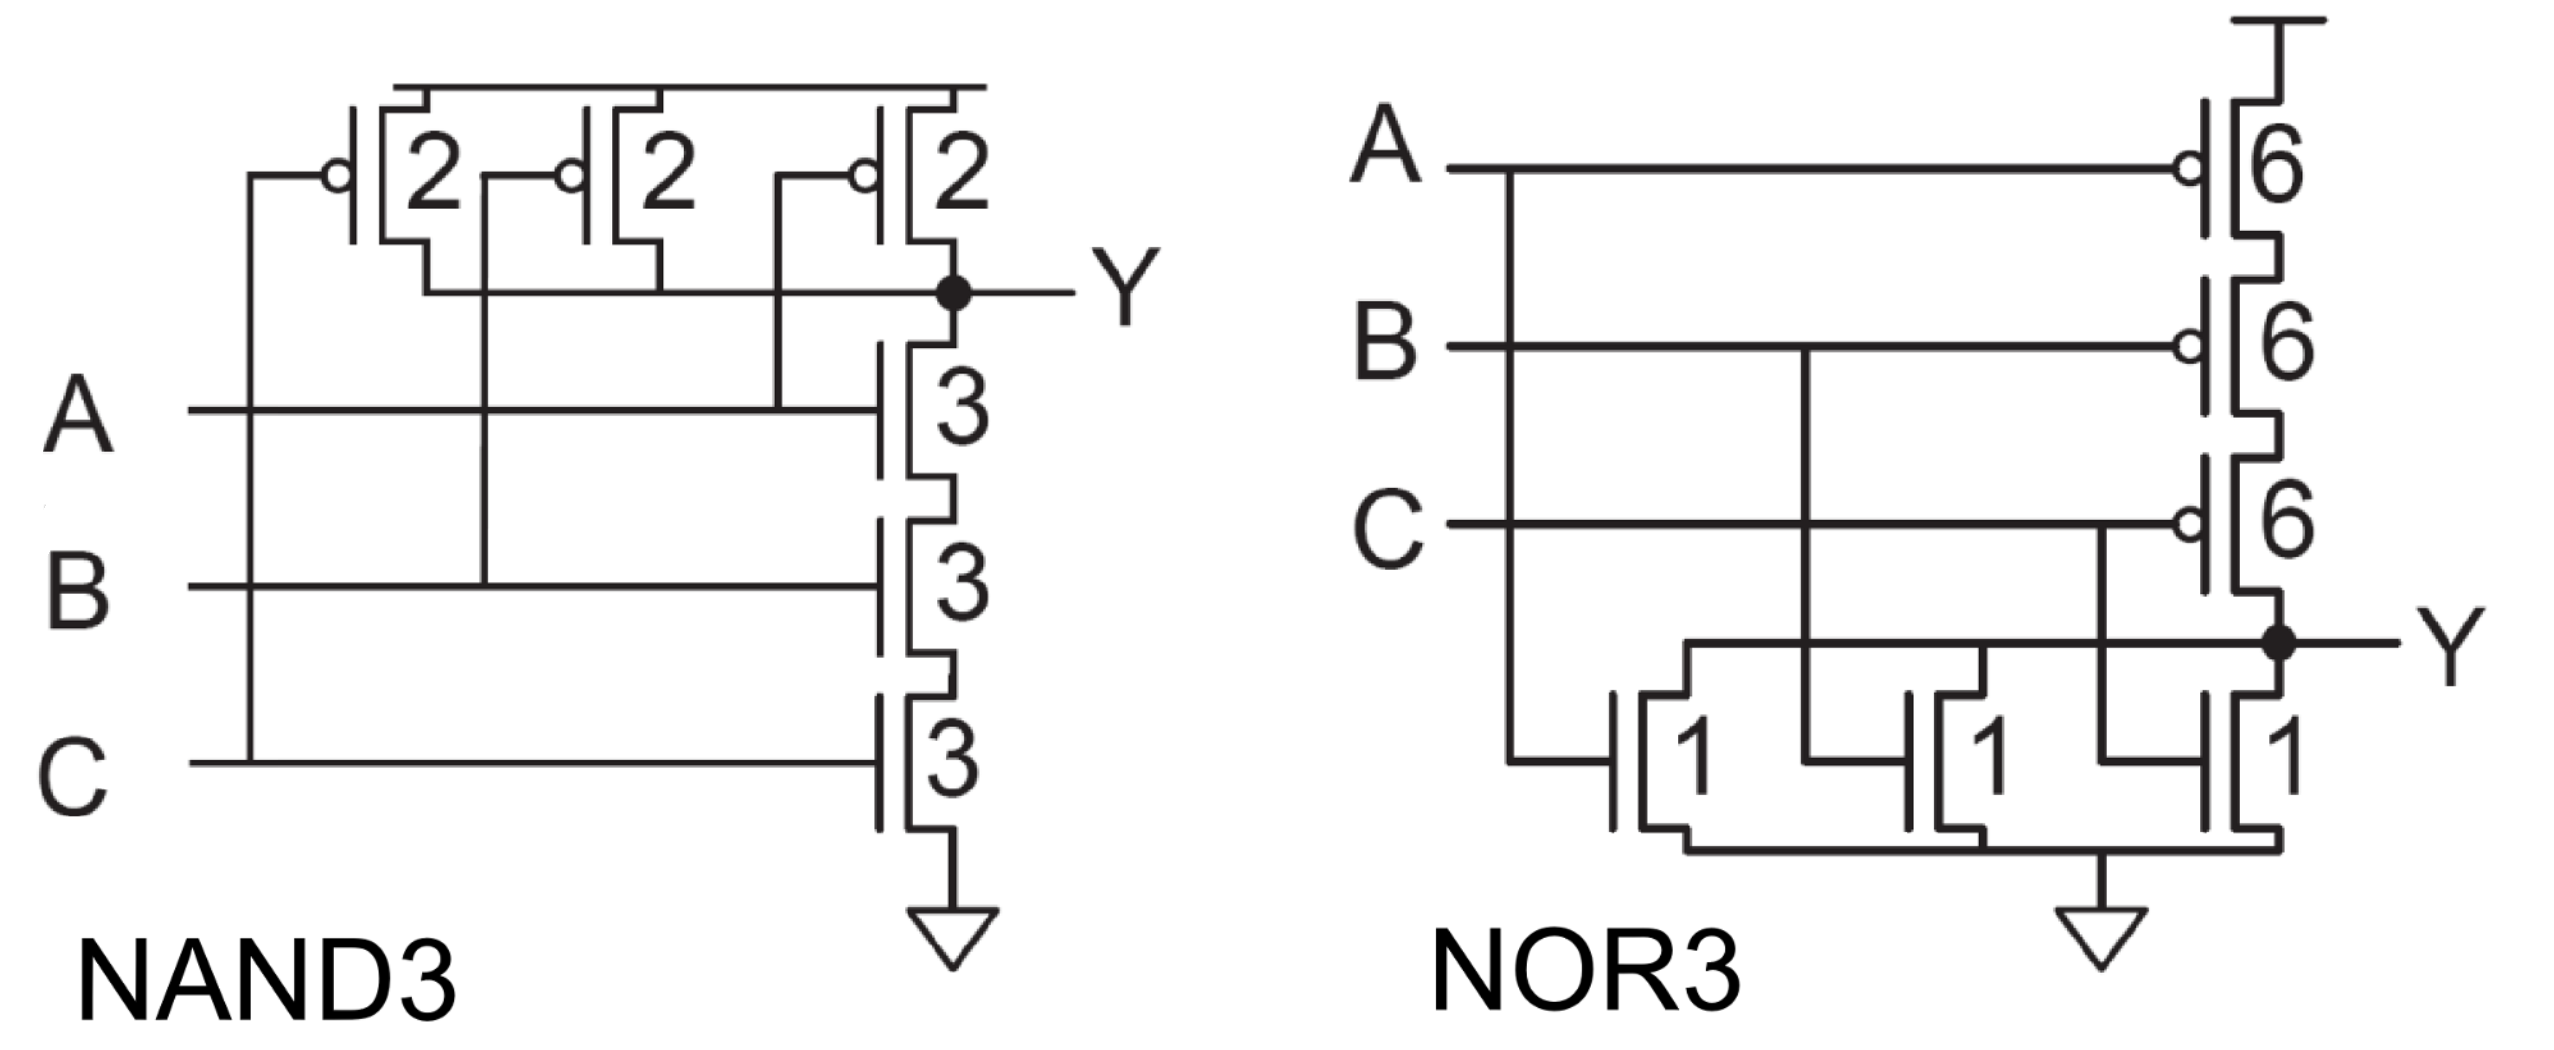
\includegraphics[width=100mm]{Sizing.png}
\caption{Sizing for NAND3 and NOR3}
\end{figure}

Consider the NAND3 case in Figure 18. In order for the route from output to ground to add up to $R_n$, each nMOS has to have a resistance of $R_n/3$. Thus the size for each nMOS is the inverse, 3. For each route from output to $V_{dd}$ to add up to $R_p$, each pMOS has to have a resistance of $R_p$ and the inverse is 1. But we multiply this size by 2 because pMOS's have to be twice as big to get the same performance.

Consider the NOR3. Each path from output to ground has a resistance of $R_n$, so a size of 1. To add up to $R_p$, each pMOS from output to $V_{dd}$ has to have a size of 3, and multiplying by two we get 6 for each. 

\begin{figure}[ht!]
\centering
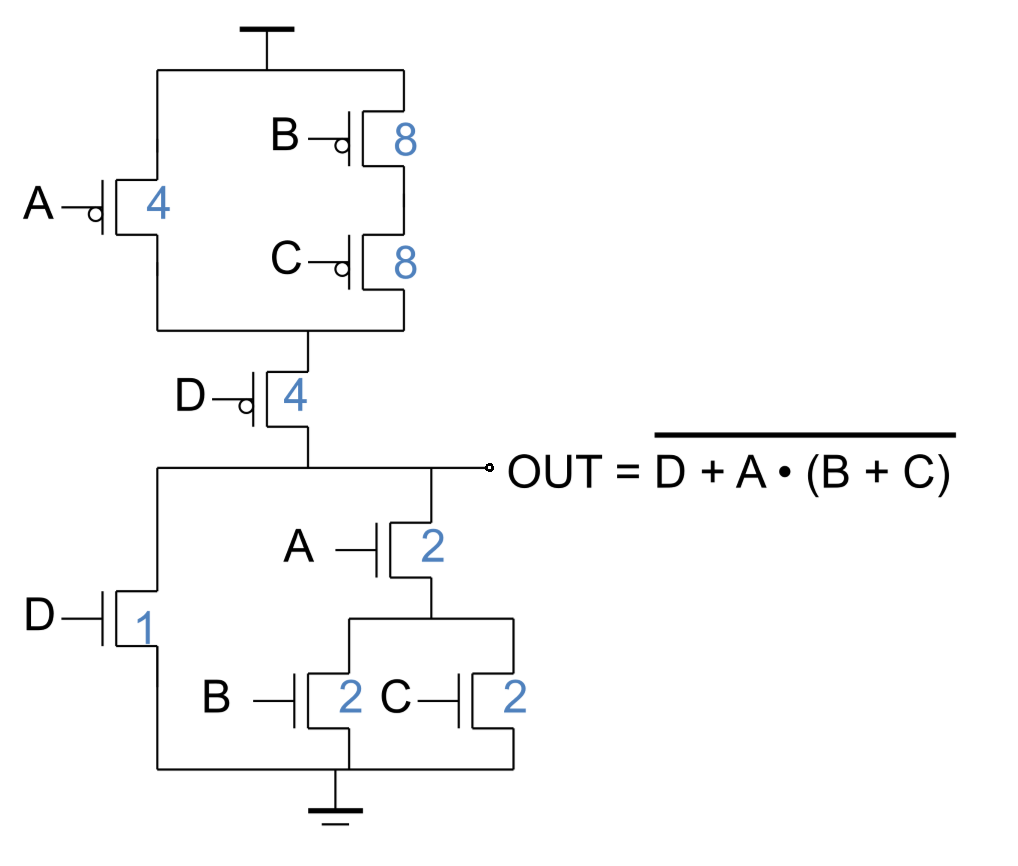
\includegraphics[width=90mm]{Sizing2.png}
\caption{CMOS and Sizing for Y=$\neg$(D+A(B+C))}
\end{figure}

Now consider the slightly more complicated circuit in Figure 19. $R_n = R_n/2 + R_n/2$ for the rightmost routes in the PDN so their sizings are 2, and $R_n = R_n$ in the leftmost route in the PDN so its sizing is 1.

For the PUN, we have $R_p = R_p/2 + R_p/4 + R_p/4$ for the rightmost route, and $R_p = R_p/2 + R_p/2$ for the leftmost route. These correspond to sizings of 4, 8, 8 and 4, 4 respectively.

Note that we are sizing these for the worst case scenario. If the nMOS transistors A, B, and C were all on. Then the resistance of the B and C would be added in parallel, and the total resistance of the route would be $^3/_4R_n$.

(...) Expand on optimal sizing.

\subsection{Equivalent Circuits and Elmore Delay}

As we discussed, this sizing is \textit{inversely} proportional to the resistance of the transistors by some factor $k$. Sizing is also \textit{directly} proportional to the capacitance of the circuit, which dictates the delay. 

The resistance and the capacitance of the transistors are shown by the their equivalent RC circuits.

\begin{figure}[ht!]
\centering
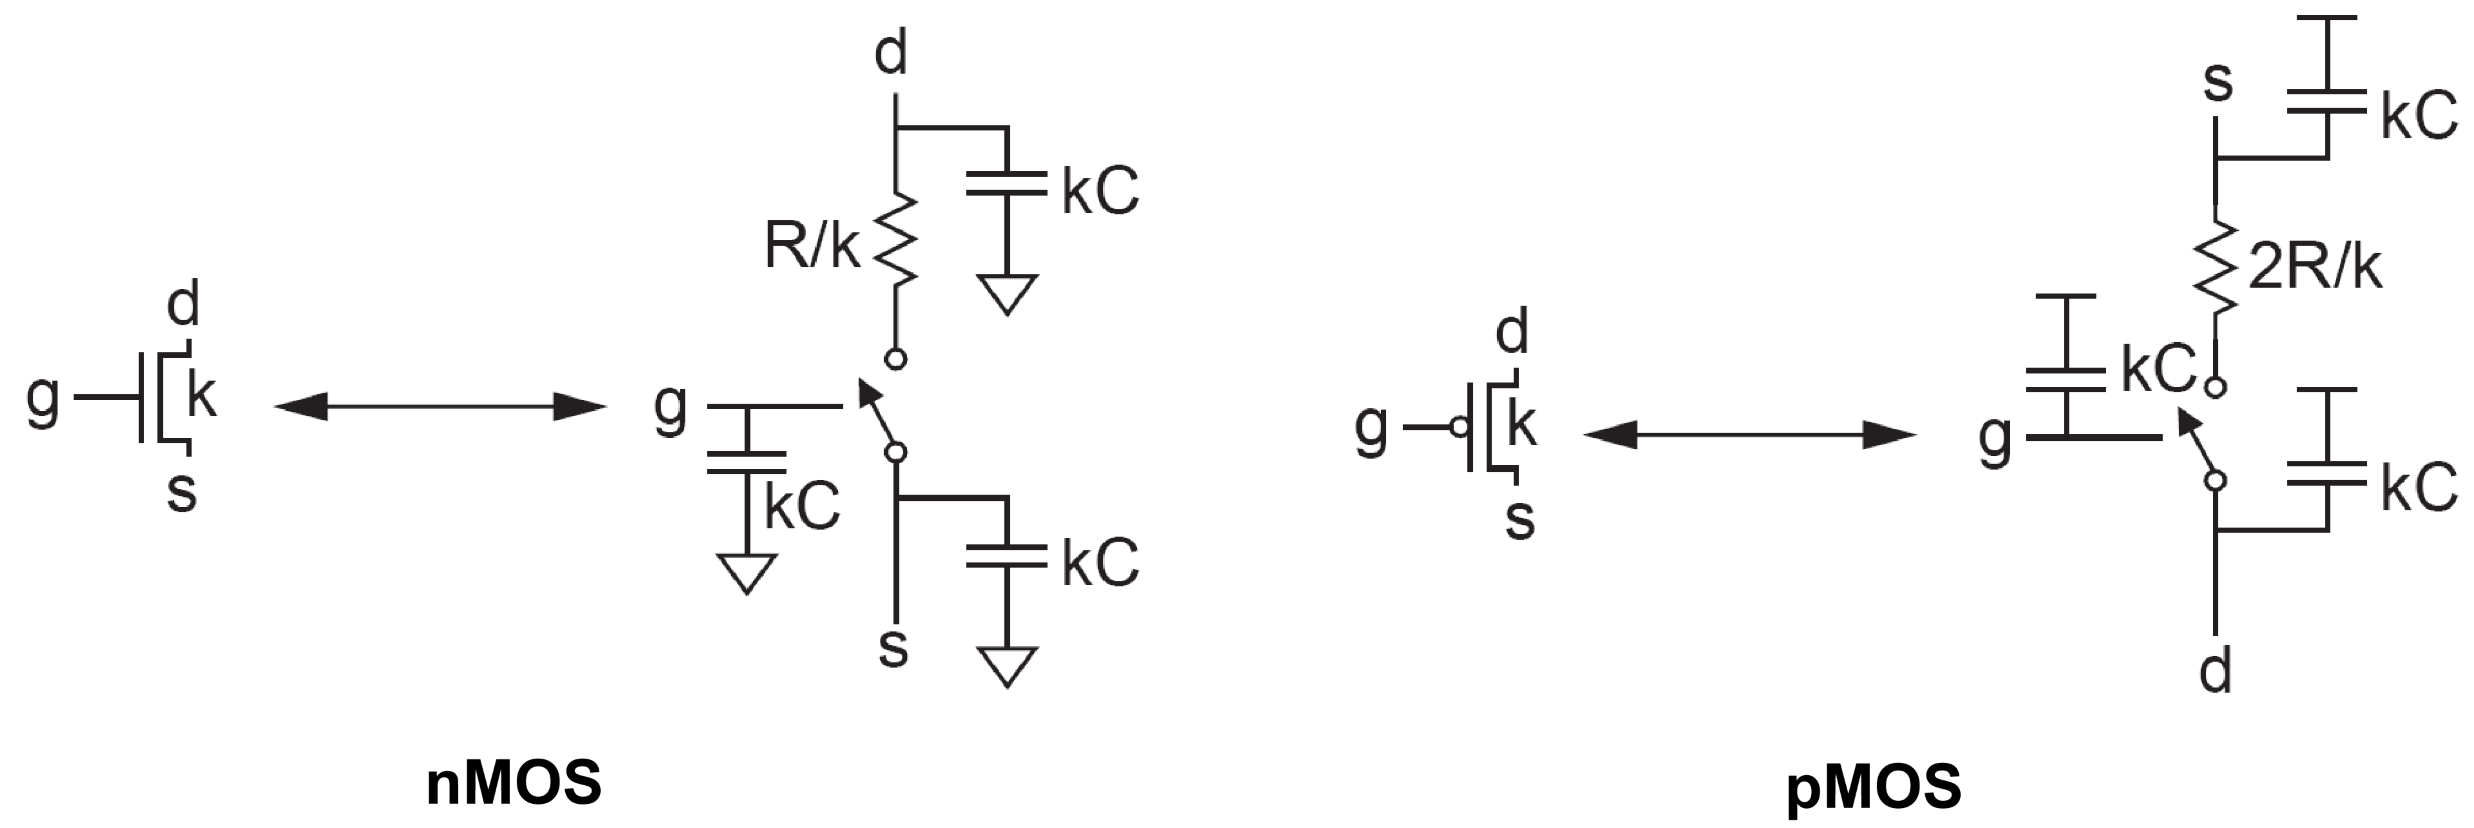
\includegraphics[width=120mm]{nMOSeq.png}
\caption{Equivalent Circuits for nMOS and pMOS}
\end{figure}

Note that when transistors are stacked in series, then in fabrication we usually lay them out such that the source of one is merged with the drain of the other. This means we can ignore the capacitance of the source terminal. 

Additionally, when the nMOS is connected to GND, the source capacitance is shorted with ground. When the pMOS is connected to $V_{dd}$ , the source capacitance is again shorted. So no matter the configuration, assuming we had the good layout shown in Figure 5, we can ignore the source capacitance.

The maximum propagation delay for a CMOS to switch output is approximated as the Elmore Delay. It is based on the resistances and capacitors on the worst-case scenario path available to charge or discharge the output. 

\begin{equation}
t_{pd} \approx R_1 C_1 + (R_1+C_2) C_2 + ... + ... (R_1+R_2+...+R_N)C_N
\end{equation}

\begin{minipage}{0.5\textwidth}
\begin{figure}[H]
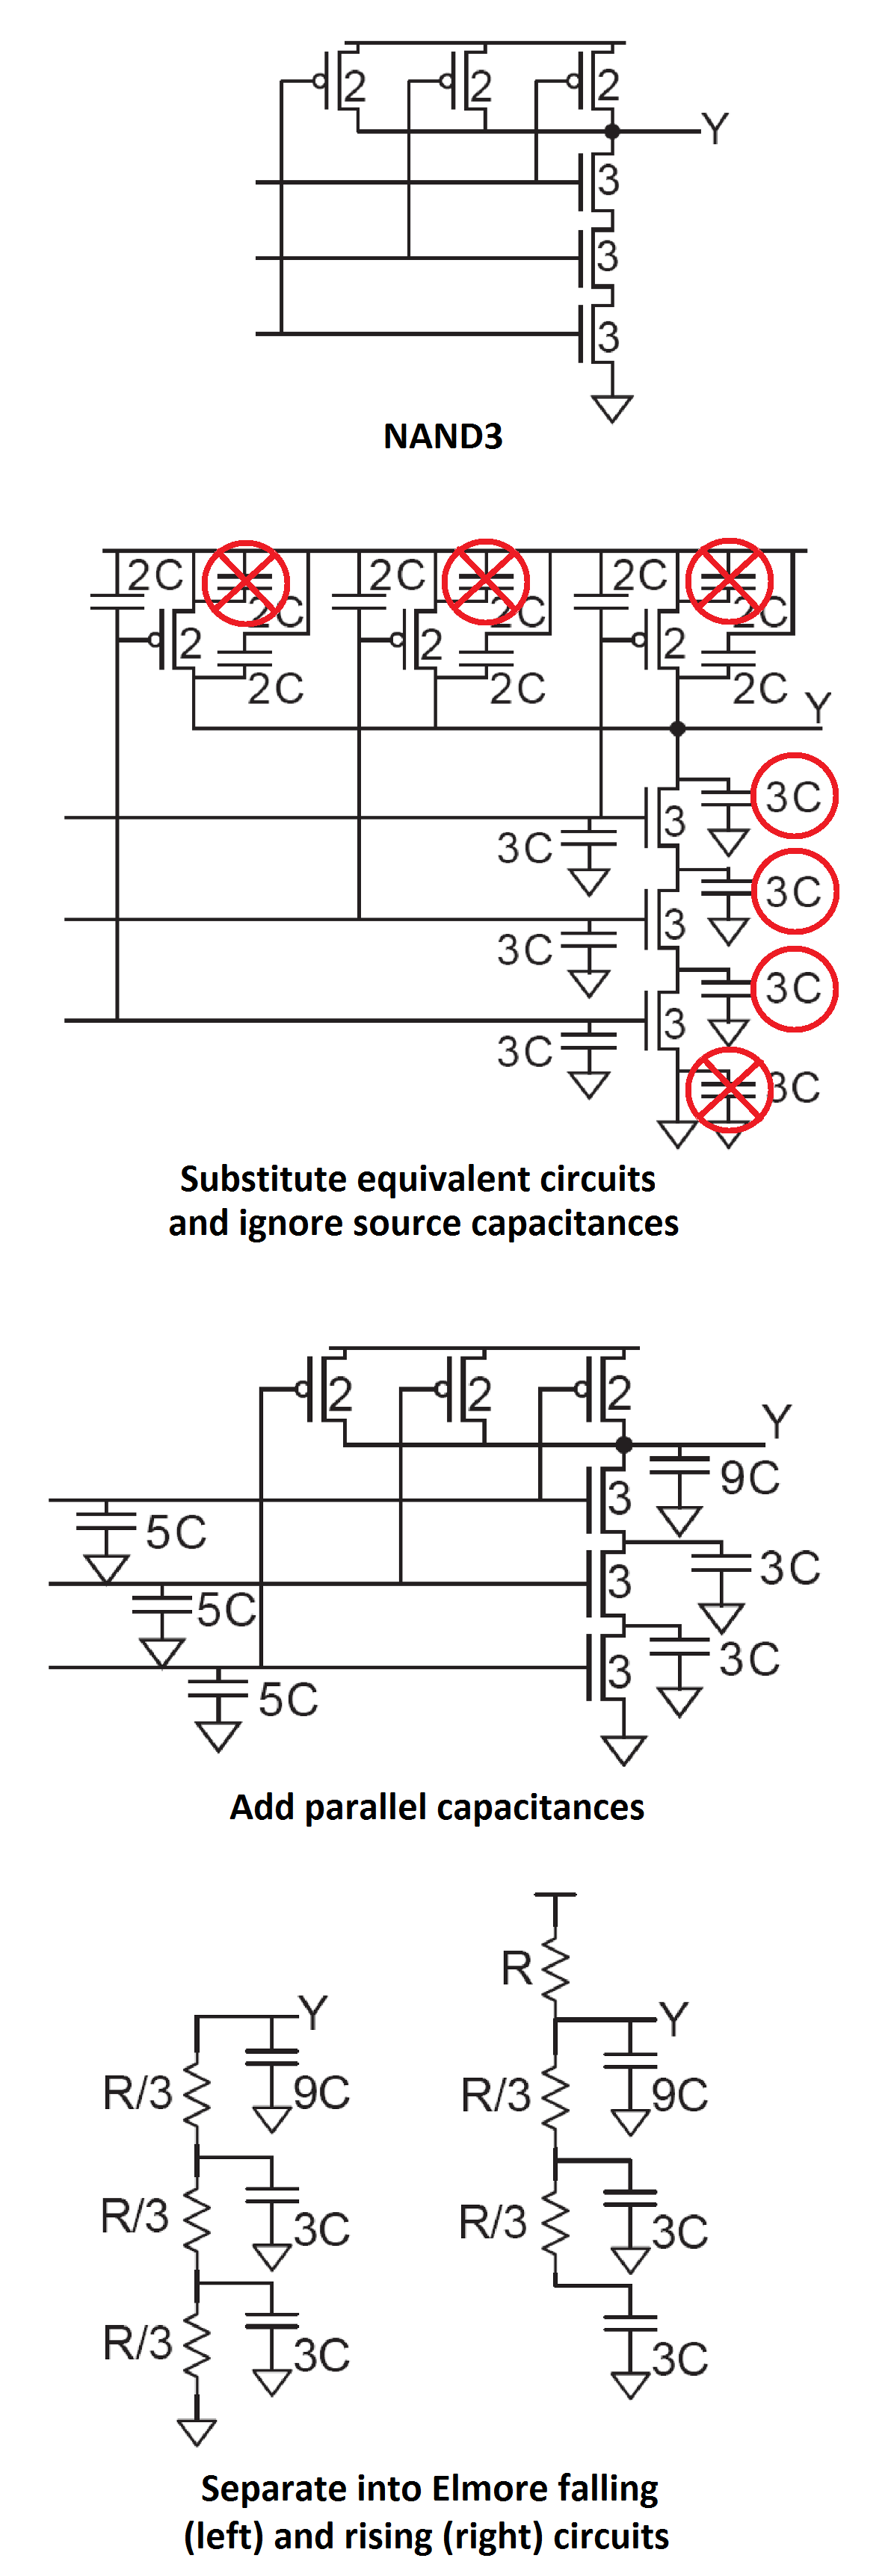
\includegraphics[width=55mm]{elmore.png}
\caption{CMOS Elmore's Delay}
\end{figure}
\end{minipage} \hfill
\begin{minipage}{0.5\textwidth}
\textbf{Example} \\


Let's walk through the steps to determine the Elmore's Delay of a CMOS circuit. 
\\

First, substitute  all the nMOS and pMOS with their equivalent circuits. The capacitance is always directly proportional to their sizing. 
\\

Recall that the source capacitance of the pMOS will be shorted to $V_{dd}$ and the source capacitance of the nMOS will be shorted to GND, so we can ignore them completely.
\\

The intermediate source capacitances of the the nMOS capacitors in series are also ignored, so the capacitance of those nodes is only the drain capacitance of each nMOS.
\\ 

We then can merge whatever remaining capacitances.

\begin{itemize}
\item The three drain capacitances of the pMOS add in parallel with the drain capacitance of the top nMOS, $2C+2C+2C+3C=9C$
\item The gate capacitances for each pair of pMOS and nMOS can also add in parallel, $2C+3C=5C$ 
\end{itemize}

Finally, we can look at the worst-case scenario level of capacitance and resistance that must be charged or discharged in order to switch the output. 
\\ 

In the worst-case scenario to charge, only one pMOS is on and it is that with the C input. In this case, there is $R$ resistance for the charge to go through from the PUN because there is only one path, and both the A and B nMOS need to be charged before the output Y is high. 

\end{minipage}

In the worst-case scenario of the example in Figure 21, the charging delay is as follows

$$t_{pd} = (R)9C+(R+\dfrac{R}{3})3C + (R+\dfrac{R}{3}+\dfrac{R}{3})3C = 18 R Cp$$

The frequency at which we can then run our circuit is then at 

$$f = \dfrac{1}{T} = \dfrac{1}{18RC}$$

\section{MOSFET Non-idealities}

Our transistors don't behave like perfect switches. Their non-idealities have effects on the following

\begin{enumerate}
\item \textbf{$\mathbf{V_{DD}}$ choice} -- We can't run them at low $V_{dd}$ values

\item \textbf{Logical effort} -- CMOS circuits driving other CMOS circuits introduce delays

\item \textbf{Power consumption} -- There's leakage 

\item \textbf{Pass transistors} -- These are bad things to use in digital circuits

\item \textbf{Temperature} -- We can't run them at very high or low temperatures
\end{enumerate}

\begin{table}
\centering
\begin{tabular}{cccc}
\toprule
& \textbf{Cutoff}  & \textbf{Linear} & \textbf{Saturation} \\
\midrule
$I_{ds}$ & 0 & $\beta\left[ ( V_{gs} - V_t )V_{ds} - V_{ds}^2/2\right]$  & $\beta\left[ ( V_{gs} - V_t )^2/2\right]$  \\
$V_{gs}$ & $<V_{t}$ & $>V_{t}$ & $>V_{t}$ \\
$V_{gd}$ & -- & $>V_{t}$ & $<V_{t}$ \\
\toprule
\end{tabular}
\caption{Shockley long-channel transistor model}
\end{table}

\subsection{Leakage}

\subsubsection{Subthreshold Leakage}

When $0<V_{gs}<V_t$, we're not actually in cutoff, we're in subthreshold region. So we will still have some current flowing. 

\section{CMOS Fabrication and Layout}

\subsection{Fabrication}

To fabricate a CMOS circuit we first lay down a p substrate. Then we add a layer of $\mathrm{SiO_2}$ as our oxide. 

\begin{figure}[ht!]
\centering
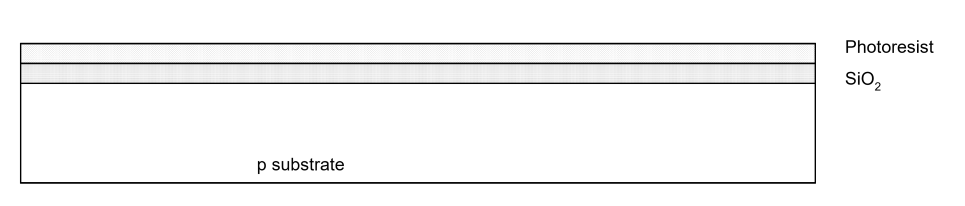
\includegraphics[width=70mm]{fab1.png}
\end{figure}


We then add a level of photoresist. This is a light-sensitive organic polymer that softens when exposed to light and can be removed. Through lithography we blast this layer with light in a pattern where we want to remove our oxide. 

Then we apply hydrofluoric acid and etch off the exposed oxide. Then we remove the remaining photoresist. 

(...)

\subsection{Layout}

When developing our CMOS gates we want to fabricate in some sort of standardized way. 

We want them to snap together easily. They must all have the same height, and have a GND at the bottom and a $V_{dd}$ at the top. They way when placed adjacently, the GND and $V_{dd}$ islands can touch and propagate. Gate inputs and outputs should snap together. 

The nMOS transistors should be placed at the bottom of the cell and the pMOS at the bottom. These should all share one continuous diffusion. 

We should use poly and only an M1 metal to route the transistors together in the CMOS circuit. Upper layer metals should be reserved for interconnecting different gates. 

All cells must follow design rule checks, DRC, otherwise lithography limitations dictate that manufacturers cannot design consistent and reliable cells. These are rules such as minimum separation between metals and separate diffusions.

\begin{figure}[ht!]
\centering
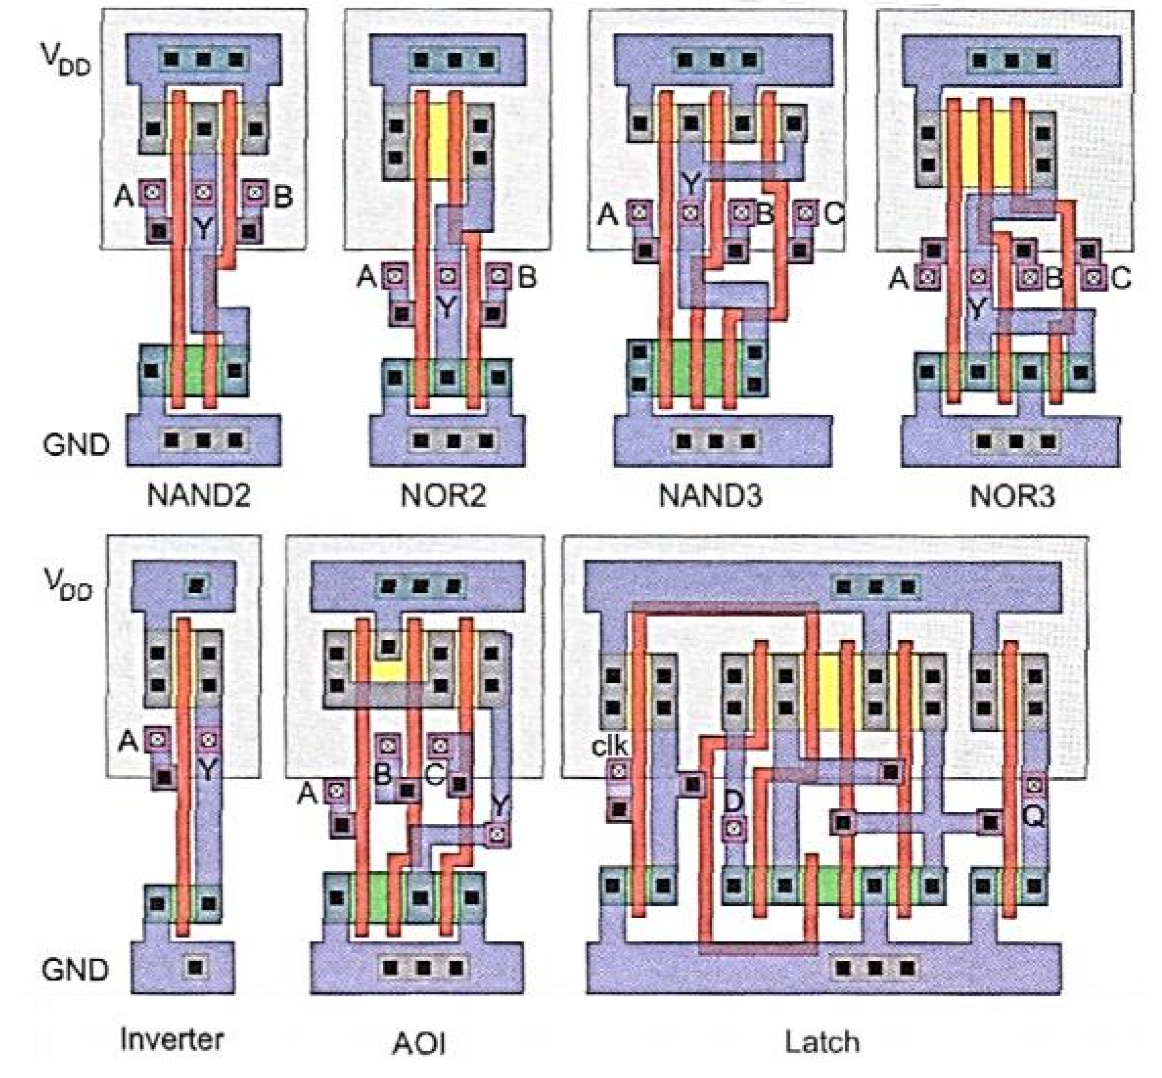
\includegraphics[width=50mm]{STD.png}
\caption{A Simple Standard Cell Library}
\end{figure}

(...)

\subsubsection{Stick Diagrams}

Stick diagrams are how digital designers can plan out a layout for a circuit, most of the methods and rules discussed above can be left to Cadence and a layout designer. 

These allow us to plan out a good layout quickly by representing the relative positions of transistors and the metal contacts between them. 


\begin{figure}[ht!]
\centering
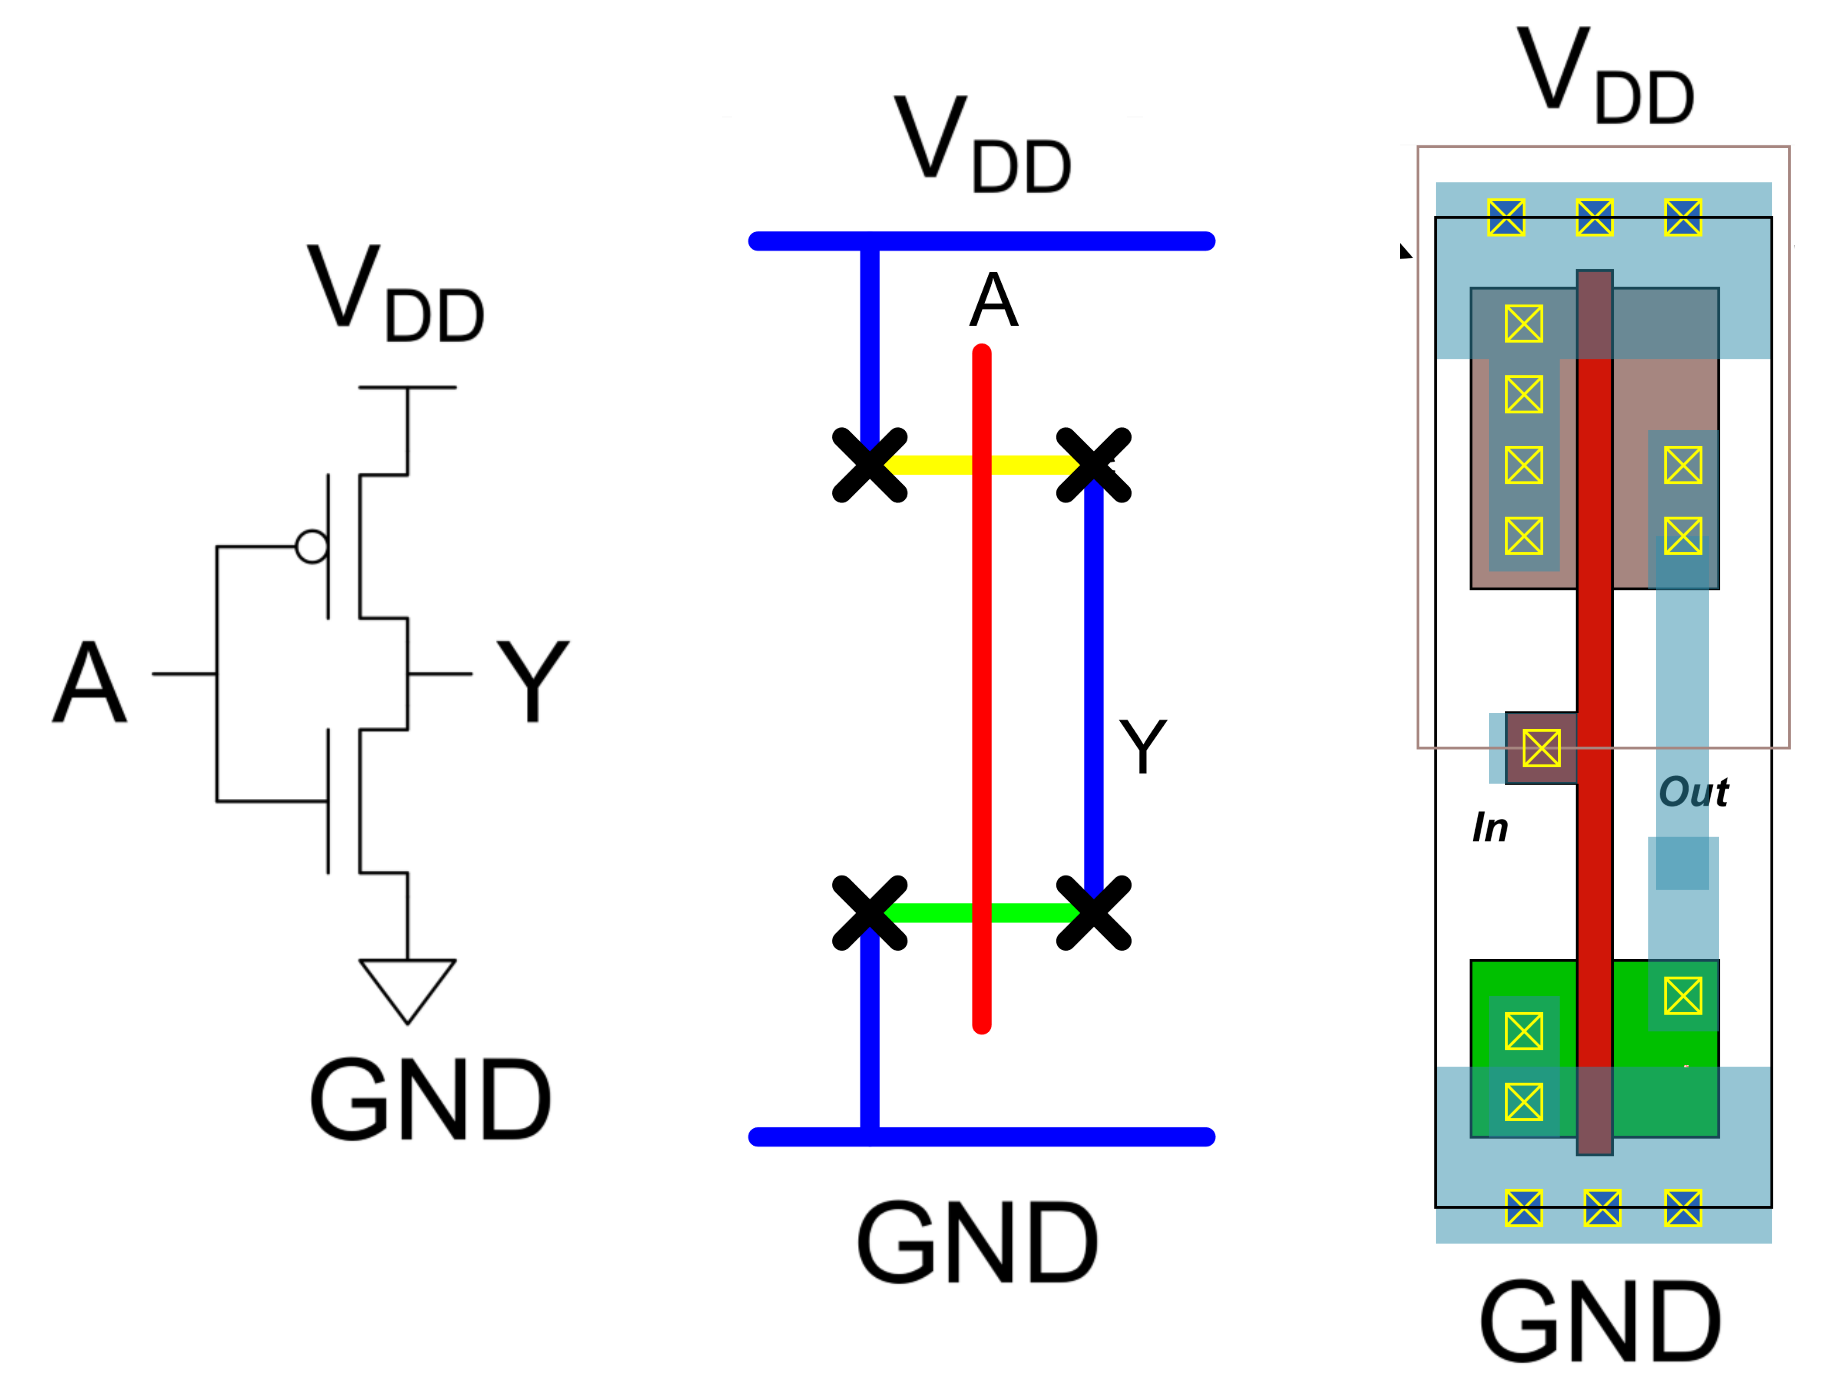
\includegraphics[width=70mm]{lyt.png}
\caption{Inverter Circuit, Stick Diagram, and Layout}
\end{figure}

The polysilicon gates are layed vertically and must be shared across the N and P type diffusions. We also must come up with a layout that allows us to have an unbroken diffusion. When there is an unbroken diffusion, the source of one transistor becomes the drain of another, so the parasitic capacitance is minimized.

This layout is determined by using some basic graph theory. An Euler path is a path that can visit each edge of a graph without revisiting any edges. 

If we treat our circuit diagram as a graph, where the transistors are edges, the route that we can draw to visit each transistor exactly once without lifting our pen of the paper is our euler path. This path is the order with which we should lay our polysilicon gates.

Let's look at an example using an OAI3 gate.

\begin{minipage}{0.5\textwidth}
\begin{figure}[H]
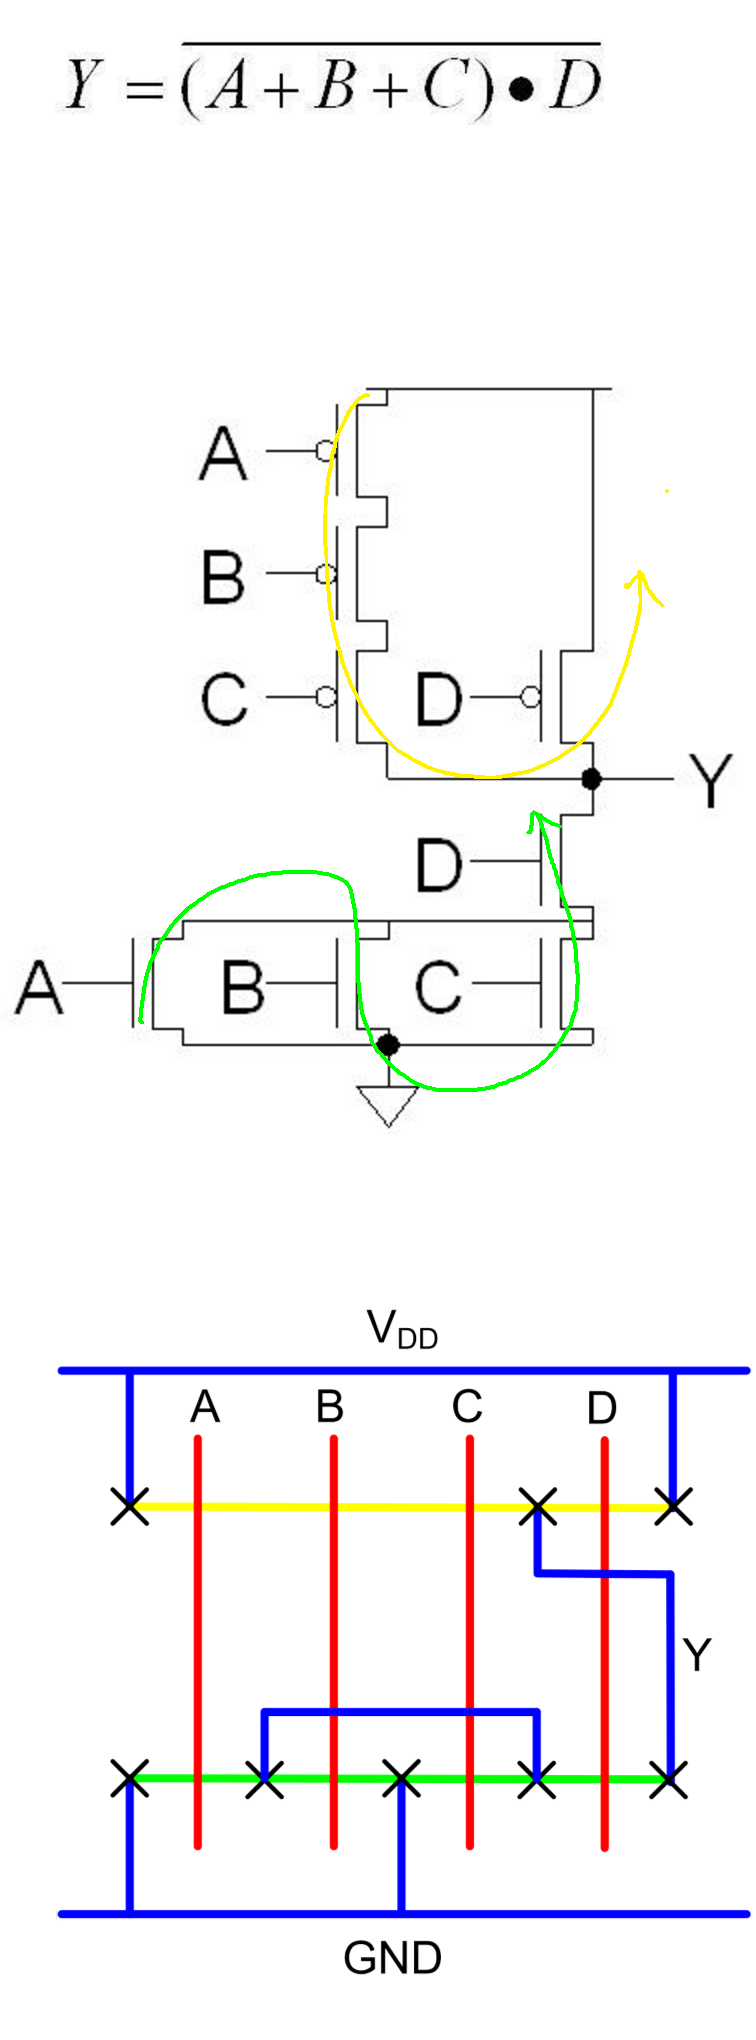
\includegraphics[width=55mm]{OAI3.png}
\caption{O3AI Stick Diagram}
\end{figure}
\end{minipage} \hfill
\begin{minipage}{0.5\textwidth}
\textbf{Example} \\

The way we laid out our CMOS PUN and PDN circuits, we can draw a line that visits each transistor exactly once. We can however revisit interconnecting nodes, including $V_{dd}$ and GND. This means that the order ABCD is our Euler path.
\\

In order to have a valid Euler path, the order we visit each transistor has to be the same in both the PUN and the PDN. You may have to modify the layout of either circuit to suit this. 
\\

To fabricate our stick diagram, we then lay out our vertical poly strips in the order of our Euler path, ABCD. Then we have to come up with the corresponding connections. 
\\

Let's start with connecting the D and ABC portions of the PDN. You have to find the nodes on the stick diagram that connect two transistors sharing a diffusion. In this case, we have the nodes AB, BC, and CD. In order to merge the AB and DC nodes as in the CMOS circuit, we draw a wire connecting them. 
\\

Then note that the other side of A, B, and C must connect to GND. Since A was the start of our Euler trail, it is not connected to another transistor, so we can directly connect that to ground. Similarly, the end of D can go directly to the output. The other side of B and C share a the BC node which we also connect to ground.
\\

In the PUN, the DC node must go to the output, so we connect that to the D of the PDN. Finally, the other side of A and D go to $V_{dd}$.


\end{minipage}
\newpage

\subsubsection{Finding an Euler Trail}

An Euler trail exists only if there are zero or two nodes that have an odd degree -- the number of edges touching that node (not including GND or $V_{dd}$. If so, you know there is a way to design your layout so it has continuous diffusion.



Try to rearrange the schematic however you can to achieve either 0 or 2 odd degree nodes. Then the Euler trail will start at one node of odd degree and end at the other node of odd degree. 

\begin{figure}[ht!]
\centering
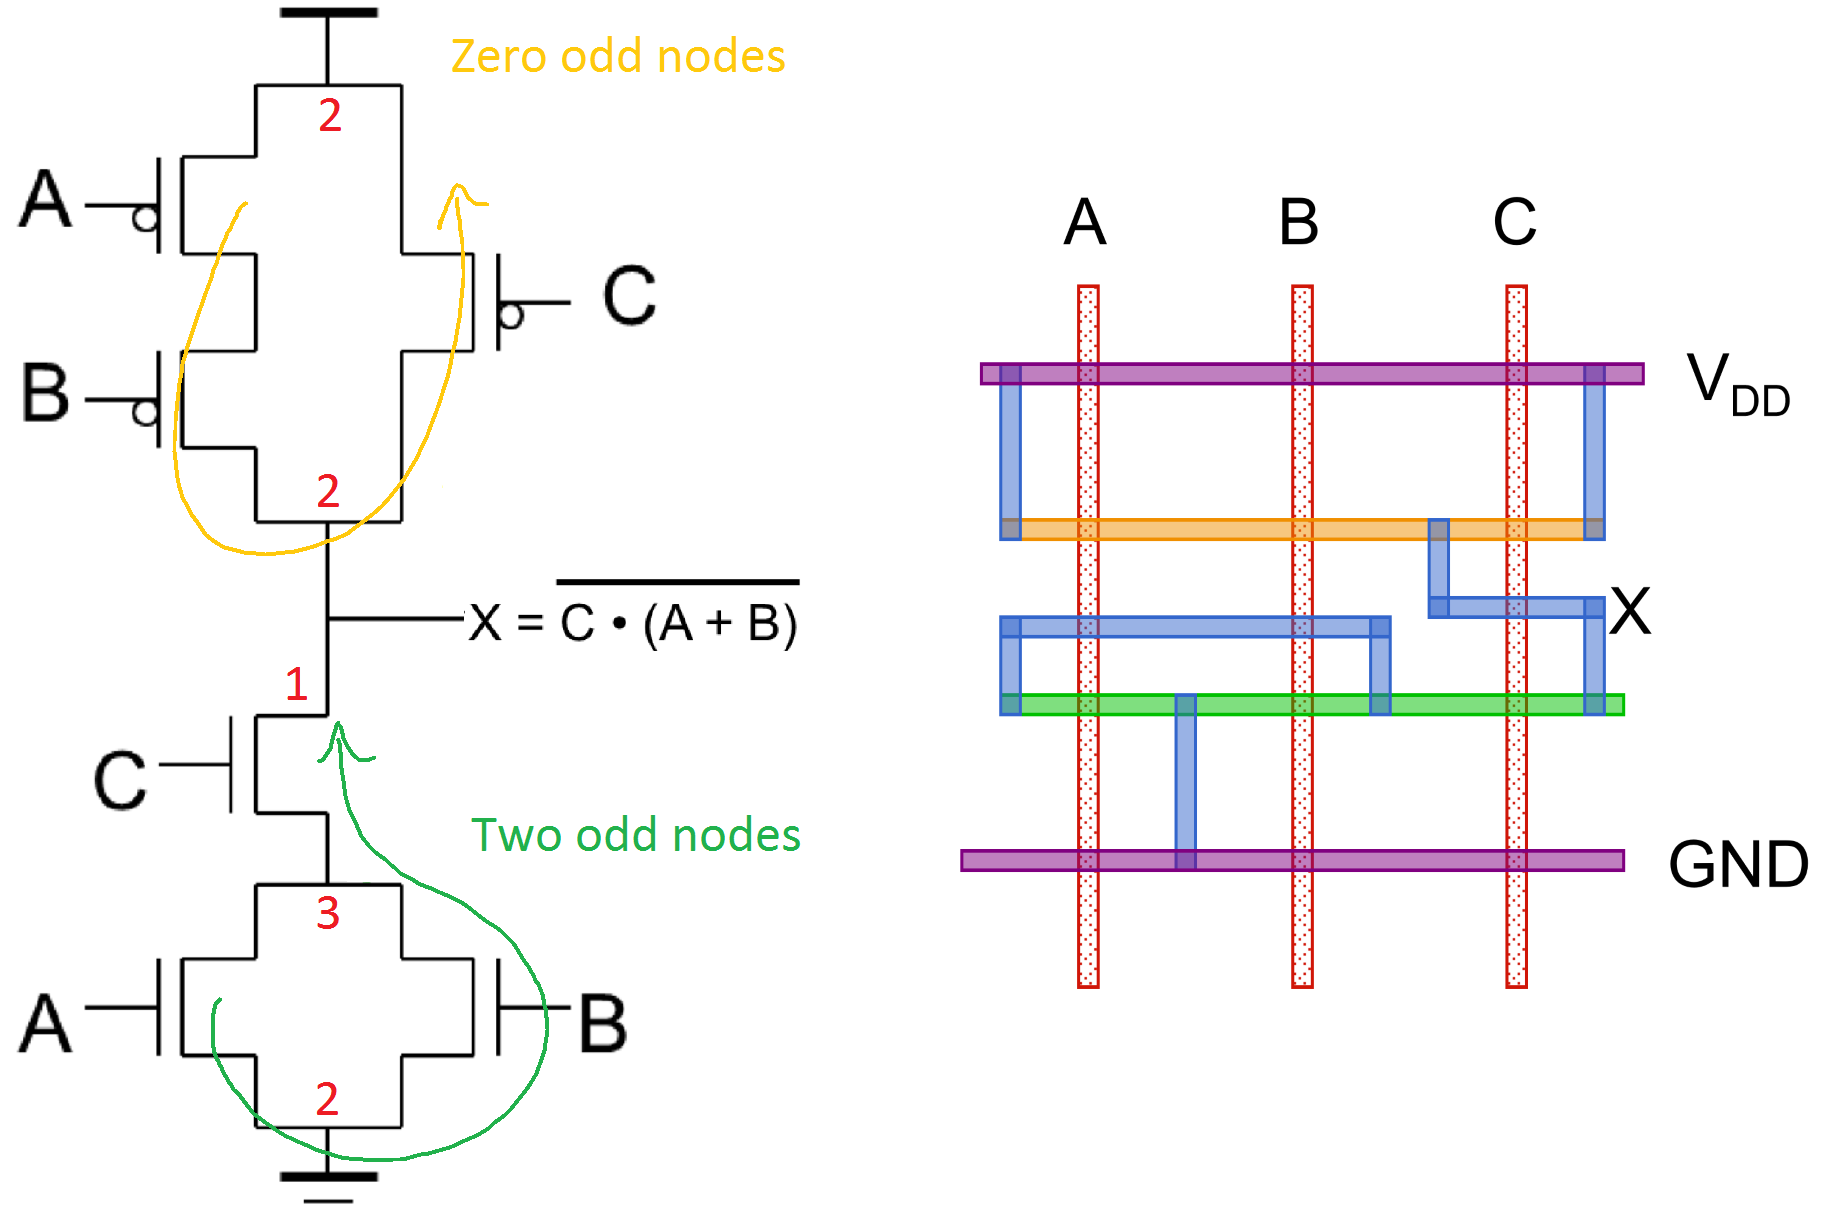
\includegraphics[width=100mm]{stick2.png}
\caption{Euler Trails and Stick Diagram}
\end{figure}

It is impossible for the sum of all degrees to equal an odd number, so if you see this, then you have incorrectly counted the degrees of your nodes.

Note that in section 7.1 I discussed how it was preferable to place single capacitors in series on the output rail to minimize output capacitance. This rule may impede our ability to create a Euler path. Preventing a broken diffusion takes precedence over minimizing output capacitance, so the circuit should be rearranged to allow for an Euler path even if this means putting parallel capacitors at the output rail.


\section{Combinational Logic Families}

Other than the static CMOS logic we have been discussing so far, there are other combinational logic families. In the past these used to be more crucial to know, but most of them are not used a lot anymore except for in the case of memory circuits where speed and density is king.

So how do you speed up a circuit? Well, propagation delay is proportional to capacitance and change in voltage, and inversely proportional to current. 

$$I = C \frac{dV}{dt} \rightarrow t_{pd} \propto \frac{C}{I} \Delta V$$

So we can try to reduce our capacitance, increase our current, or reduce our voltage swing. The main enemy here is capacitance, and the PMOS is the guilty party. They're big, capacitive, and and slow, so most of these families revolve around getting rid of PMOS. 

\subsection{Pseudo-NMOS}

Pseudo-NMOS is faster than CMOS, but it has static power consumption. It is used in NOR-based structures like ROMs and PLAs (programmable logic arrays). 

It is similar to CMOS, except for the PUN use one PMOS that is always on. This means that when the output should go low and the NMOS network creates a path to ground, the PMOS  continues to drive the output with $V_{dd}$, causing contention. 

However, we design the PMOS to be weak (small) so  that the NMOS current flows faster than the PMOS current. Thus the output capacitance  discharges through the  NMOS faster than it charges through the PMOS, so when we get logical contention the output can still go low. This means we consume static power whenever the output is low.

But low is not GND with pseudo-NMOS. The PMOS is charging the output and the NMOS is discharging the output faster, but NMOS transistors cannot fully transmit the high signal so the remaining low output is $V_t \approx 200mV$. 

\begin{equation}
\begin{matrix}
V_{hi} = V_{dd} \\
V_{lo} = V_t \\
\end{matrix}
\end{equation}
\myequations{Pseudo-NMOS Voltage Swing}

Pseudo-NMOS is faster because we only have one PMOS and the PMOS is smaller, so we have less capacitance. The input also only goes to the NMOS so the input capacitance is also reduced. Finally, the voltage swing is not fully from GND to $V_{dd}$.


If you make the PMOS too small, charging the output capacitance takes too long. If the PMOS is too big, it lets too much current flow which is current passed directly from $V_{dd}$ to GND, which is wasted static power. 



\begin{equation}
V_{out} = V_{dd} \frac{R_{PDN}}{R_{PDN} + R_{PUN}}
\end{equation}
\myequations{Pseudo-NMOS output voltage}

In order to make sure the discharge rate is the same in the PMOS and the PDN, the PMOS should be about 1/4 of the effective strength of the NMOS network. That is, the resistance (the inverse of the width) of the PMOS network should be 2x that of the NMOS network.


\begin{figure}[ht!]
\centering
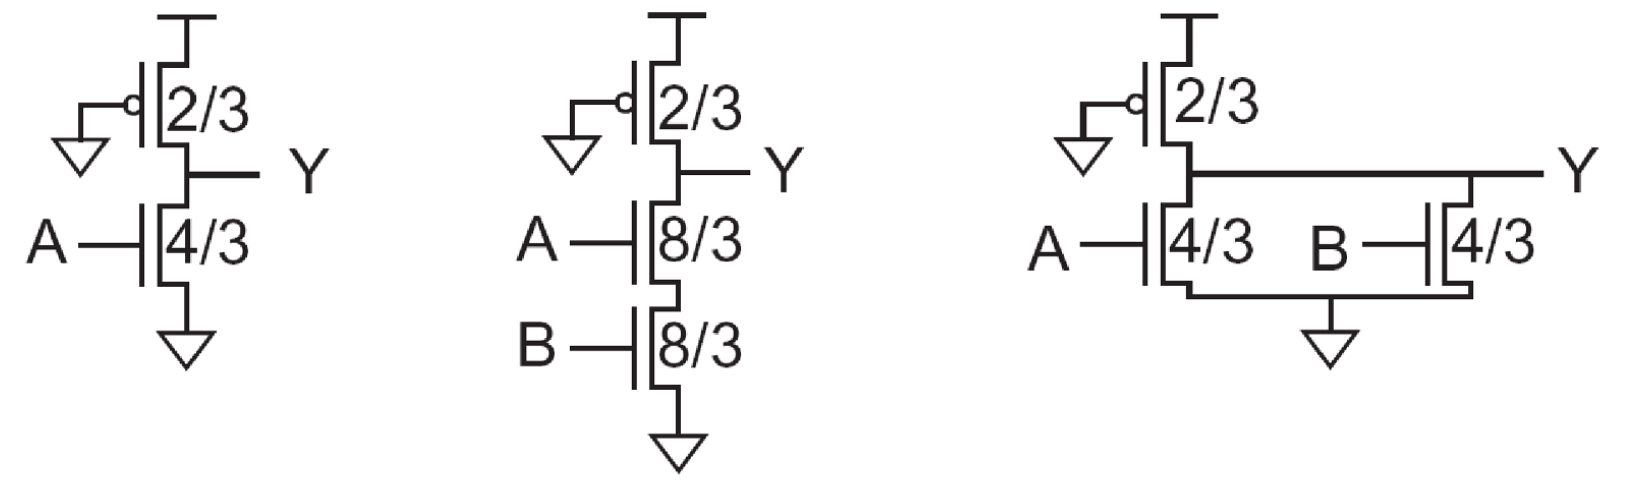
\includegraphics[width=100mm]{Pseudo.png}
\caption{Pseudo-NMOS Inverter, NAND2, and NOR2}
\end{figure}

For an inverter, this simply means that the PMOS should be 1/2 of the width. For two NMOS in series, each NMOS has to be twice as large. In the case of the NAND2, this means that $R_{PDN} = \frac{3}{8}+\frac{3}{8} = \frac{3}{4}$, which is 1/2 as large as $R_{PUN} = \frac{3}{2}$. 

For NMOS in parallel like a NOR2, they have to be sized the same as the inverter for the worst case scenario where only one NMOS is on. These circuits should be used sparingly for circuits that need to be fast, don't have power restrictions, and have wide NOR gates.

In order to reduce the static power consumption, rather than connecting the PMOS gate directly to GND, you can connect it to an enable bit which only turns the PMOS on when the gate is in use. This prevents leakage current when the gates are not in use. 

\subsection{Dynamic Logic}

Dynamic logic uses a clocked pullup PMOS so we have two modes: precharge ($\phi=0$) and evaluate ($\phi=1$). 

Before evaluation, we turn on the PMOS and precharge the output to $V_{dd}$, this way we don't have to wait for it to charge if the input is supposed to be high. During evaluation, we turn off the PMOS, and the output can remain high (by dynamically storing preserving charge in the output capacitance) or it will be discharged low through the NMOS network. 

\begin{figure}[ht!]
\centering
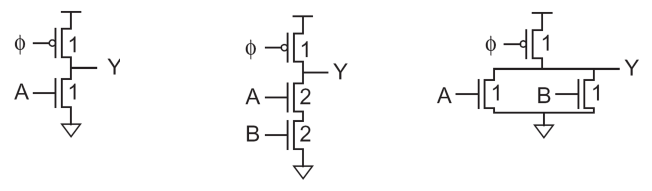
\includegraphics[width=100mm]{Unfooted.png}
\caption{Dynamic-Logic Inverter, NAND2, and NOR2}
\end{figure}

Since we precharge the output while the gate is idle, we don't have to size the PMOS as large because it can take longer. We size it for twice the unit resistance of the NMOS network. Since its smaller we can reduce the capacitive load of the clock.

During precharge, if the inputs are such that the NMOS network creates a path to ground, then there will be contention at the output which consumes static power. In order to avoid this, a clocked NMOS transistor can be placed at the bottom of the NMOS network. This is called the foot transistor.
\
\begin{figure}[ht!]
\centering
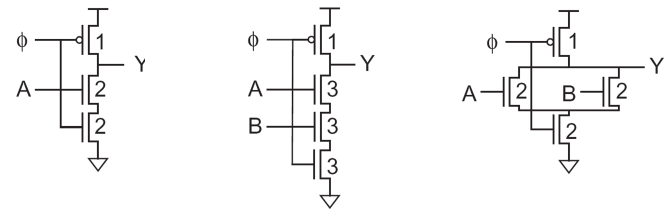
\includegraphics[width=100mm]{Footed.png}
\caption{Dynamic-Logic Inverter, NAND2, and NOR2}
\end{figure}

Dynamic logic is very fast because there is lower input capacitance since the input is only provided to the NMOS. With the foot, it does not consume any static power, but consumes significant dynamic power. Dynamic logic are also susceptible to input noise, because if an NMOS transistor is accidentally turned on momentarily, the charge on the output is lost, whereas with CMOS it would be continually driven by $V_{dd}$. 

For this same reason, dynamic logic cannot be driven at a low frequency. Transistors will leak and dynamic logic, that is logic that is stored in capacitors, will eventually discharge if not refreshed. The minimum frequency is dependent on the leakage, and the maximum frequency is dependent on how fast the output node can discharge during evaluation.

Leakage can be mitigated by using a keeper transistor and an inverter. This can be used reinforce the high charge of a dynamic node ("staticize"). However, it must be very weak -- only strong enough to counteract leakage, but easily overpowered by input logic. 

\begin{figure}[ht!]
\centering
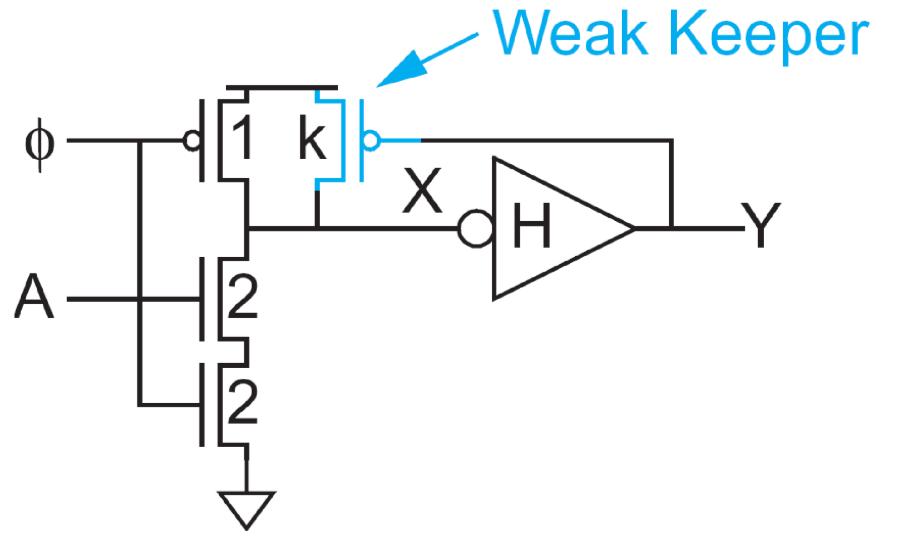
\includegraphics[width=50mm]{keeper.png}
\caption{Dynamic Gate (Domino) with a Keeper}
\end{figure}

(??? We said that dynamic-logic doesn't consume static-power. Is that only true with the foot? Without the foot we could get contention, and isn't that static power consumption?)

\subsubsection{Monotonicity}

On of the challenges with dynamic logic gates is that they require monotonically rising inputs during evaluation. That is during evaluation, the inputs can stay at 0, they can stay at 1, or they can transition from 0$\rightarrow$1. However, the inputs cannot transition from 1$\rightarrow$0 during evaluation.


\begin{figure}[ht!]
\centering
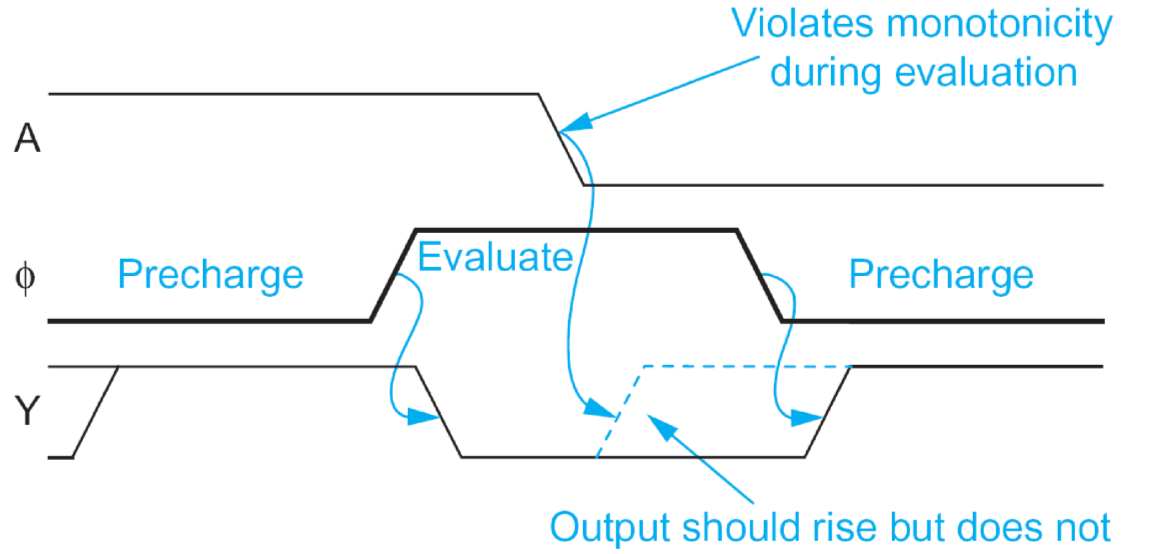
\includegraphics[width=100mm]{Mono.png}
\caption{Monotonocity Violation with Dynamic Logic}
\end{figure}



(??? is this example just for an inverter's input? Do they mean in general that because the clocked PMOS is off during evaluate, that the output can't rise, and this example is just an inverter's input. Or is there something I'm not getting.)

For this reason, dynamic gates cannot drive one-another, because they precharge the output to 1 and then may let it discharge to 0. Because of the delay between the output changing at the first gate would mean that the input of the second gate would fall during the evaluate stage, violating monotonicity. 

To overcome this, we can use domino logic. 

\subsection{Domino Logic}

We can overcome the monotonicity problem by placing static CMOS inverters between dynamic gates. This pair of dynamic gate and static inverter is a domino gate.


\begin{figure}[ht!]
\centering
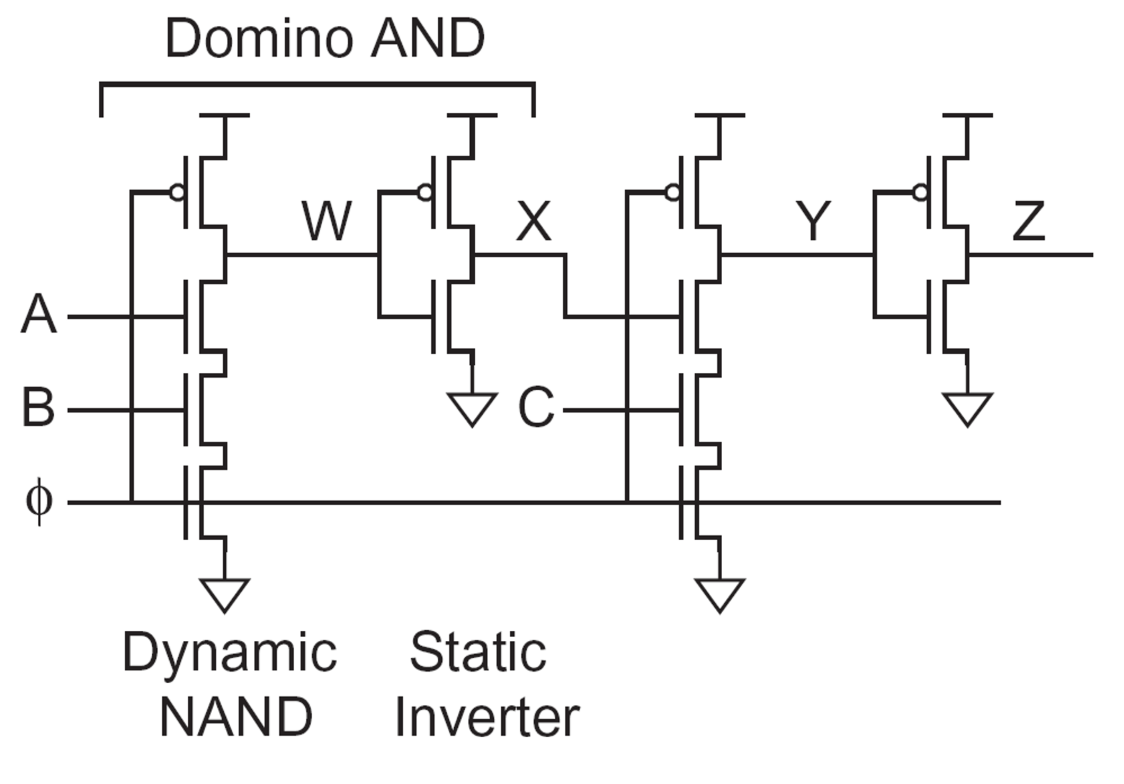
\includegraphics[width=50mm]{domino.png}
\caption{Sequential Domino AND Gates}
\end{figure}



 This means that falling outputs from the dynamic gate due to the precharge/discharge in evaluate is turned into a rising output by the static inverter. This way dynamic gates can be used to drive each other. This is why it's called domino, because the gates evaluate sequentially, each triggering the next one.
 
 Since this 1$\rightarrow$0 case is the common case for the dynamic gate, the static CMOS inverter is usually HI-skew to favour the rising output.
 
 It also means domino logic gates only create non-inverting functions, such as AND and OR functions. Whereas they cannot create inverting functions such as NAND, NOR, or XORs without intermediate static logic.  
 
 Domino gates have very high activity factors because the output toggles from high (precharge) to low approximately half the time, leading to very high dynamic power consumption, with challenges such as noise, leakage, and monotonicity. However, they are 1.3-2x faster than static CMOS. 
 
 During the 1990s, speed was the primary goal of processors and domino-logic saw its glory days, but since power is the limiting factor in more recent processors, static CMOS has largely replaced it except in some memory technologies for area efficiency.
     
\subsection{Pass-Transistor Logic}

Pass transistor circuits will be the first time we see inputs applied to the source/drain of transistors, rather than just the gate.

Here we use an NMOS and a PMOS in parallel with their gate inputs being complimentary -- called a transmission gate. These transmission gates can transfer a 1 or a 0 equivalently, so they can be used as a switch. This can be particularly efficient in the case of multiplexers. 

\begin{figure}[ht!]
\centering
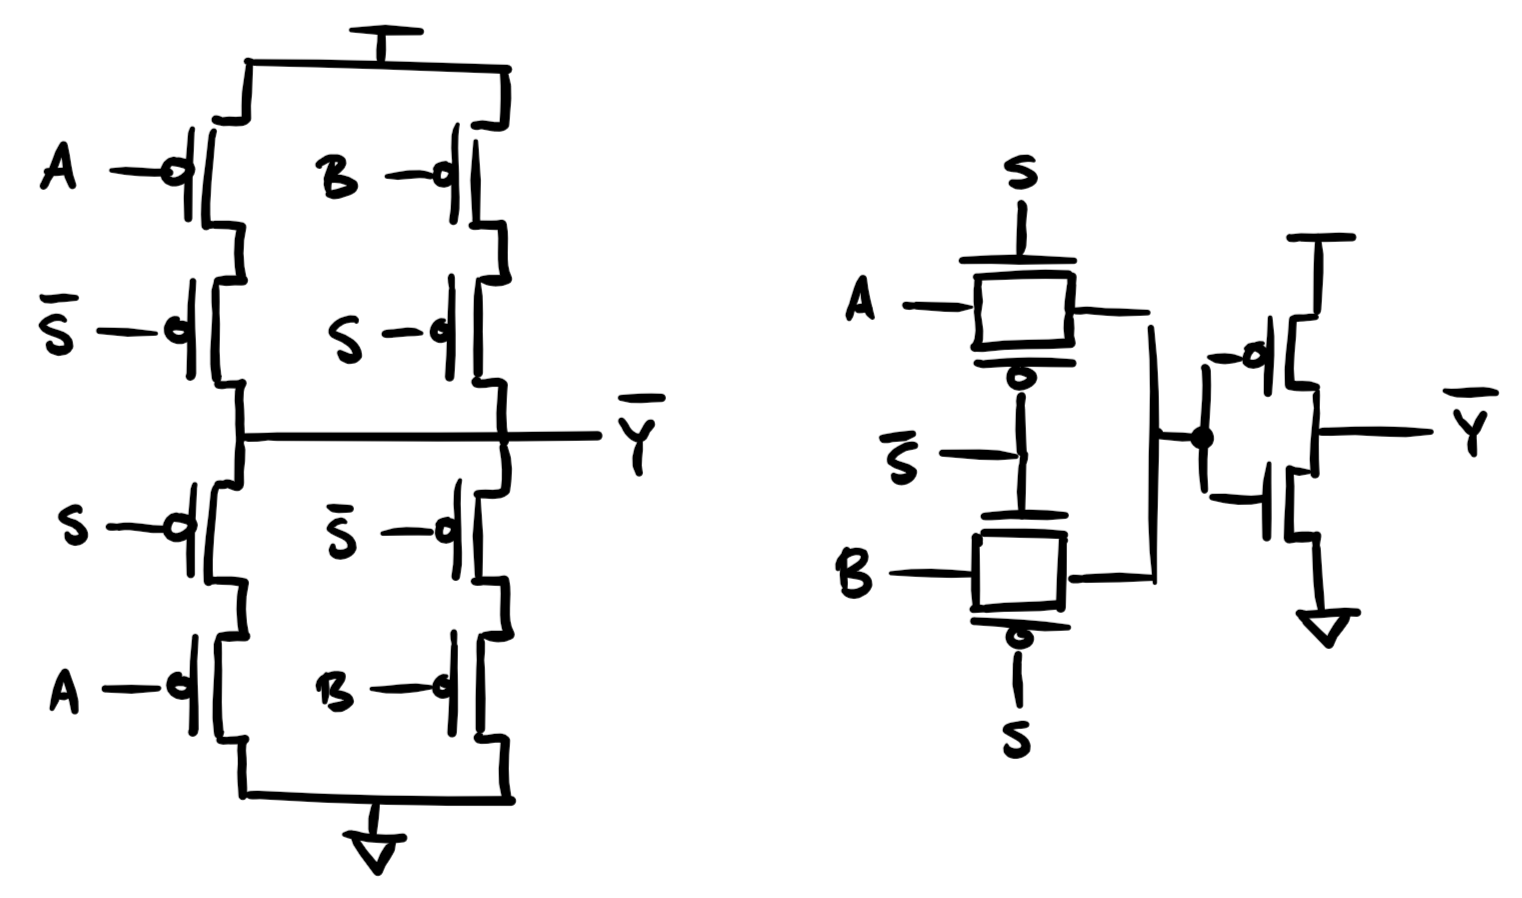
\includegraphics[width=110mm]{trans.png}
\caption{2-Input Mux with CMOS (Left), Pass-Transistor Logic (Right)}
\label{PassTrans}
\end{figure}

Note that in this case, the inputs A and B are what driving the logic. With static CMOS, the output is driven from $V_{dd}$ or GND, with pass-transistor logic, they A or B inputs cannot be driven by a weak or far away signal. If the output is high, there is even a risk that the output could discharge backward and act as a two-way propagator. 

To prevent backwards driving through the transmission gates, we attach the inverter on the output seen in Figure \ref{PassTrans}. 

Although there are some possible benefits to pass-transistor logic over CMOS, generally they are not worth it and are only used in niche circuits such as memory or XOR circuits.

---

Since memory is period, you can design something clever and specialized and copy it 1000 times and be confident it works. However, when doing logic, the gates are placed by a synthesizer and not custom-designed. This is why CMOS prevails for most logic, but the logic families described in this section can be applied to memory networks.  

\section{Sequential Logic}

In combination logic, such as the gate networks we have described so far, the output only depends on current inputs. In sequential logic, the output depends on the inputs as well as previous inputs -- having some state. Notable examples of sequential logic are finite state machines (FSMs) and pipelines.

\begin{figure}[ht!]
\centering
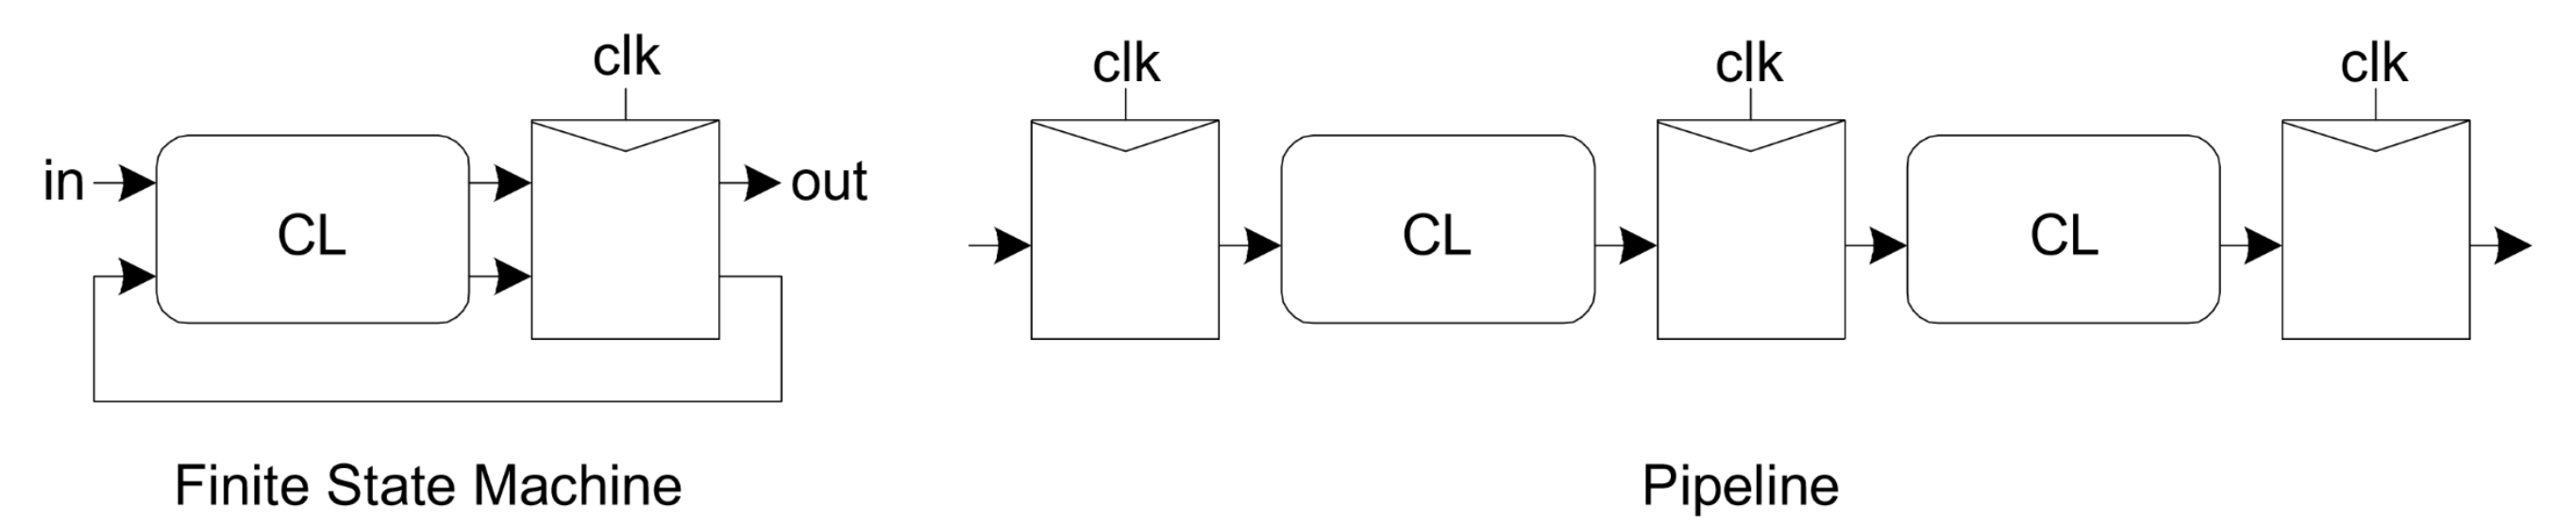
\includegraphics[width=110mm]{seq.png}
\caption{Finite State Machine and Pipeline Sequential Logic}
\end{figure}

We use sequential logic over combination logic because combinational logic has some glitches, sequential logic can have parallelized operations in different parts of the circuit, then those different operations can be synchronized to arrive at another part of the circuit simultaneously.

We get the benefits of sequential logic at the cost of speed because we add some delay other than just the logic delay, and at the cost of area because we use flip-flops or latches, called sequencing elements.

Latches are level-sensitive, whereas flip-flops are edge-triggered. We say that a latch is transparent when the clock is high, and opaque when the clock is low. This is because while the clock is high, a latch will propagate whatever input it is given. When the clock is low, a latch behaves more like a flip-flop, preserving its output until the clock goes high again. 


\begin{figure}[ht!]
\centering
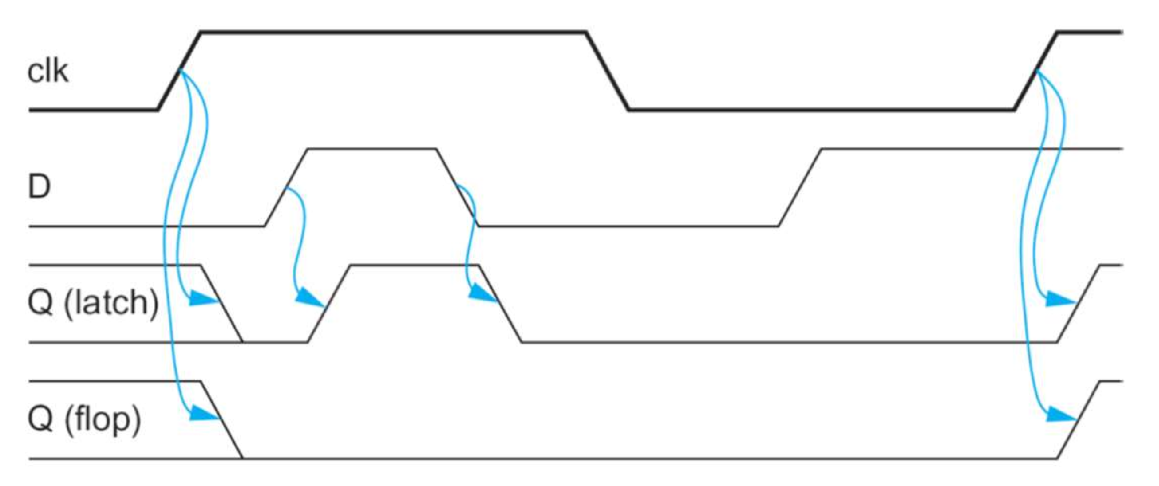
\includegraphics[width=90mm]{latchff.png}
\caption{Difference Between Latch and Flip-Flop}
\end{figure}

The flip flop will only change its output on the clock edge (usually rising), and will propagate the value it is provided with at that moment (an oversimplification, we will elaborate in the following section). 

\subsection{Latches}

\subsubsection{Dynamic Latches}

The most simple latch is simply an NMOS pass transistor, where the clock is connected to the gate. When the clock is high, it is transparent. When the clock is low, the output is preserved with the capacitance at the output. The pros of this are of course that the latch is small and the load for the clock  is small. 

Also obvious are the cons of this: there is a $V_t$ drop when the NMOS transmits a 1; the value stored at the output can leak and can't be restored; a noise event at the output can propagate backwards (backdriving); and the input is driven by an unknown signal rather than being buffered/reinforced by an inverter (a diffusion input) so it is also sensitive to noise at the input.

\begin{figure}[ht!]
\centering
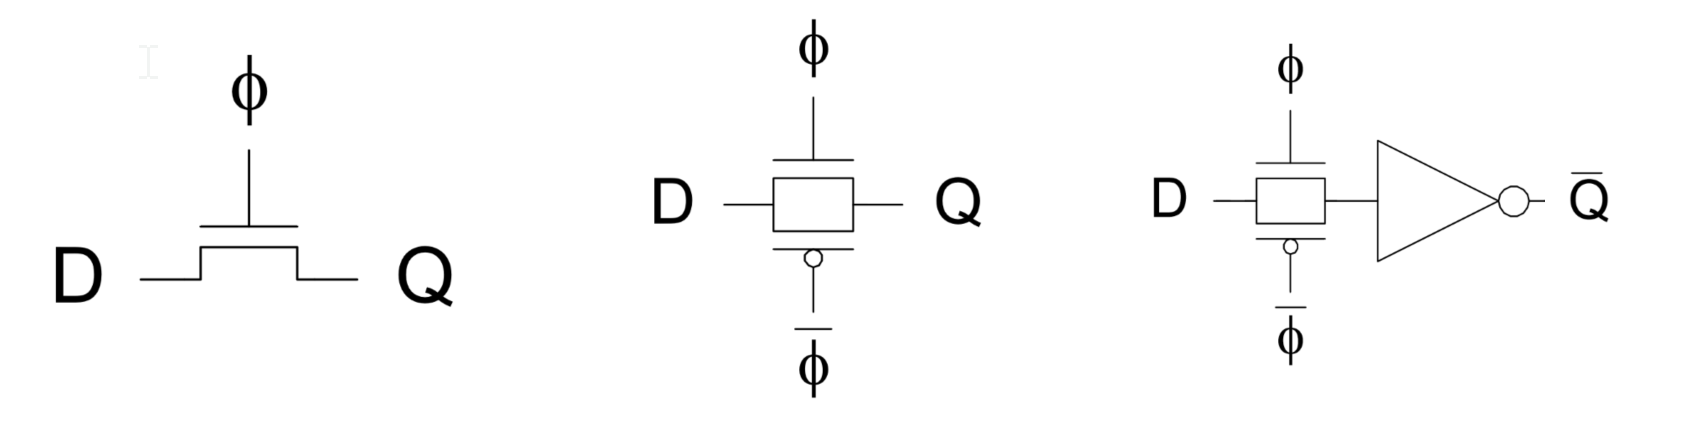
\includegraphics[width=90mm]{StaticLatch.png}
\caption{Dynamic Latches}
\end{figure}

By adding a PMOS transistor we can avoid the $V_t$ drop, but require an inverted clock. Then if we add an inverting buffer at the output, we can prevent backdriving because the inverter will drive the output from $V_{dd}$ or GND. Or if we add an inverter at the input we can fix our diffusion input. But the intermediate value will still be stored dynamically.  



\subsubsection{Static Latches}

Now that transistors are so small, leakage is more of a concern. In the past they could get away with dynamic logic because the transistors weren't as leaky, but nowadays static logic is essential -- that is, the logic at every node is driven. The other bonus, is that static logic can be driven at any frequency because you don't have to worry about charges leaking. 

Static latches require some sort of feedback. The most basic design simply uses back-to-back inverters to reinforce the stored value. Here we use a clocked-inverter as the feedback. 

This inverter only drives the output when the clock is low, $\phi=0$. The reason it is clocked is because the node $X$ will be driven by both the input $D$, and the output $\overline{Q}$. If there is a change at the input, contention will happen at $X$ before the latch inverters update. So when $\phi=1$, we are in transparent mode in the transmission gate, and the feedback inverter is off so there is no contention, then when $\phi=0$ we are in opaque mode and the feedback is reinstated. 


\begin{figure}[ht!]
\centering
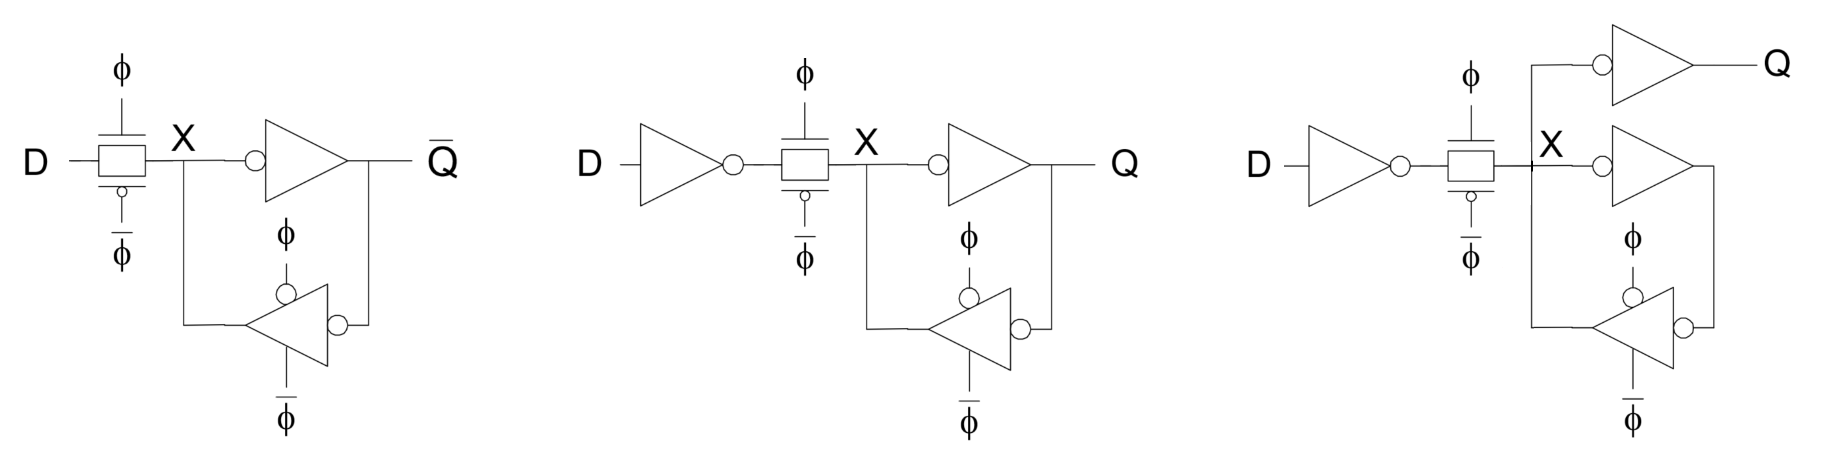
\includegraphics[width=110mm]{StaticLatches.png}
\caption{Static Latches}
\end{figure}

If we add another inverter to the input, we can avoid our input diffusion and make our latch less sensitive to input noise. This has the added bonus of making the latch non-inverting. 

However, the latch is still vulnerable to backdriving to the $X$ node through the feedback inverter. So for our final fix we take our input from $X$ and passing it through another inverter so the output is not connected to the feedback inverter. 

This latch is widely used in standard cells and is very robust. The downsides are that its somewhat large and slow, and is a high load for the clock. 

\subsubsection{Clocked Inverter/$\mathbf{C^2MOS}$ Latch}

The clocked inverter discussed in the previous section is called a C2MOS latch. It should be designed with the clocked transistors connecting to the output, rather than to GND and $V_{dd}$. 

\begin{figure}[ht!]
\centering
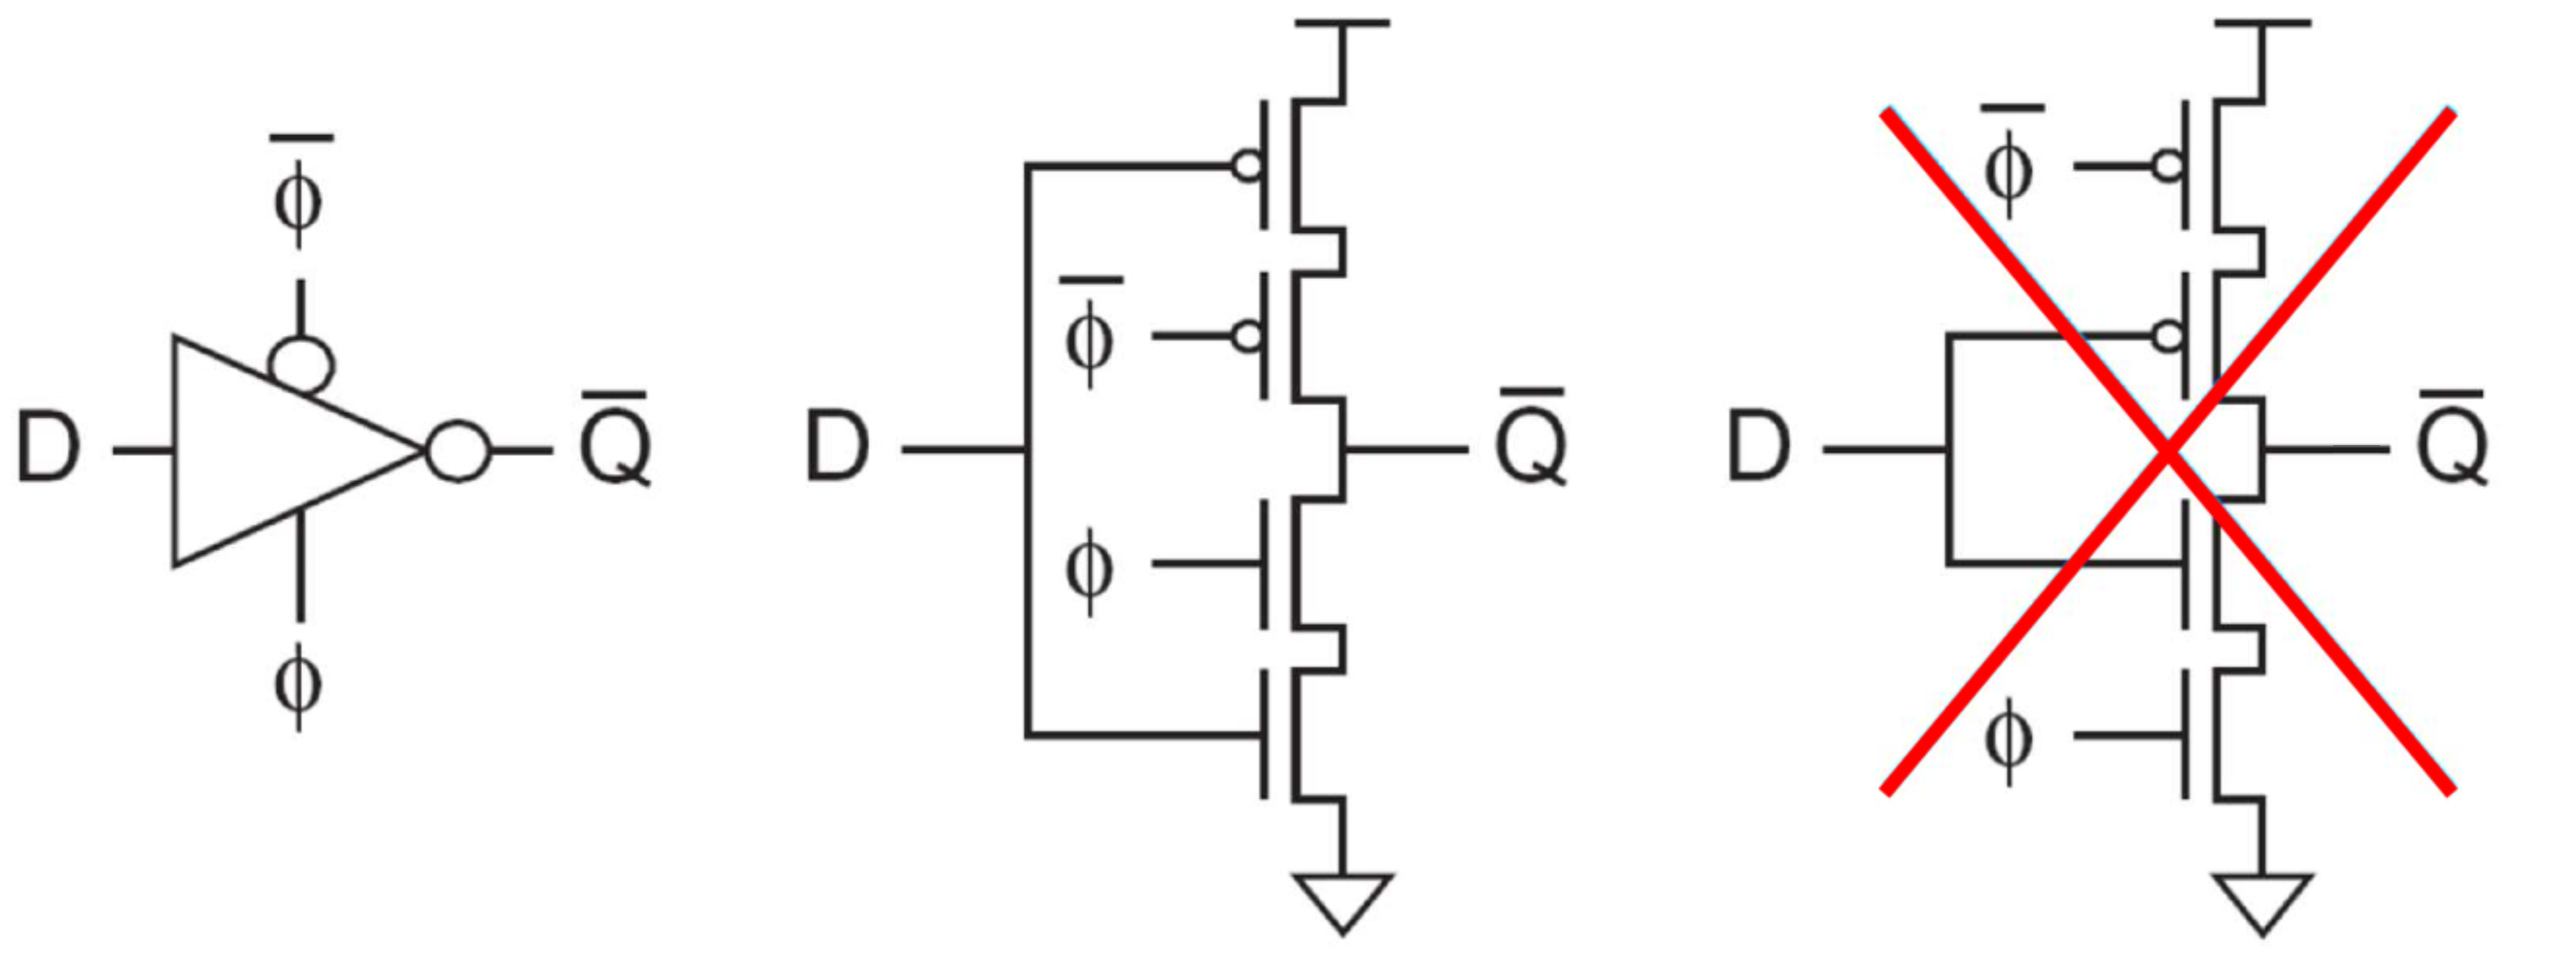
\includegraphics[width=90mm]{C2MOS.png}
\caption{C2MOS Latch}
\label{C2MOS}
\end{figure}

When transparent ($\phi=1$), the C2MOS latch should act as an inverter, and when opaque ($\phi=0$) the C2MOS latch should store the previous value. With the design on the right of Figure \ref{C2MOS}, if the output starts as charged to 1 and then $\phi \rightarrow 0$, the output should stay at 1. 

However, since of the transistors connected to D will be on, even though there won't be a connection to GND or $V_{dd}$, the output node will distribute its charge across the on transistor, depleting the output charge somewhat. 

\begin{figure}[ht!]
\centering
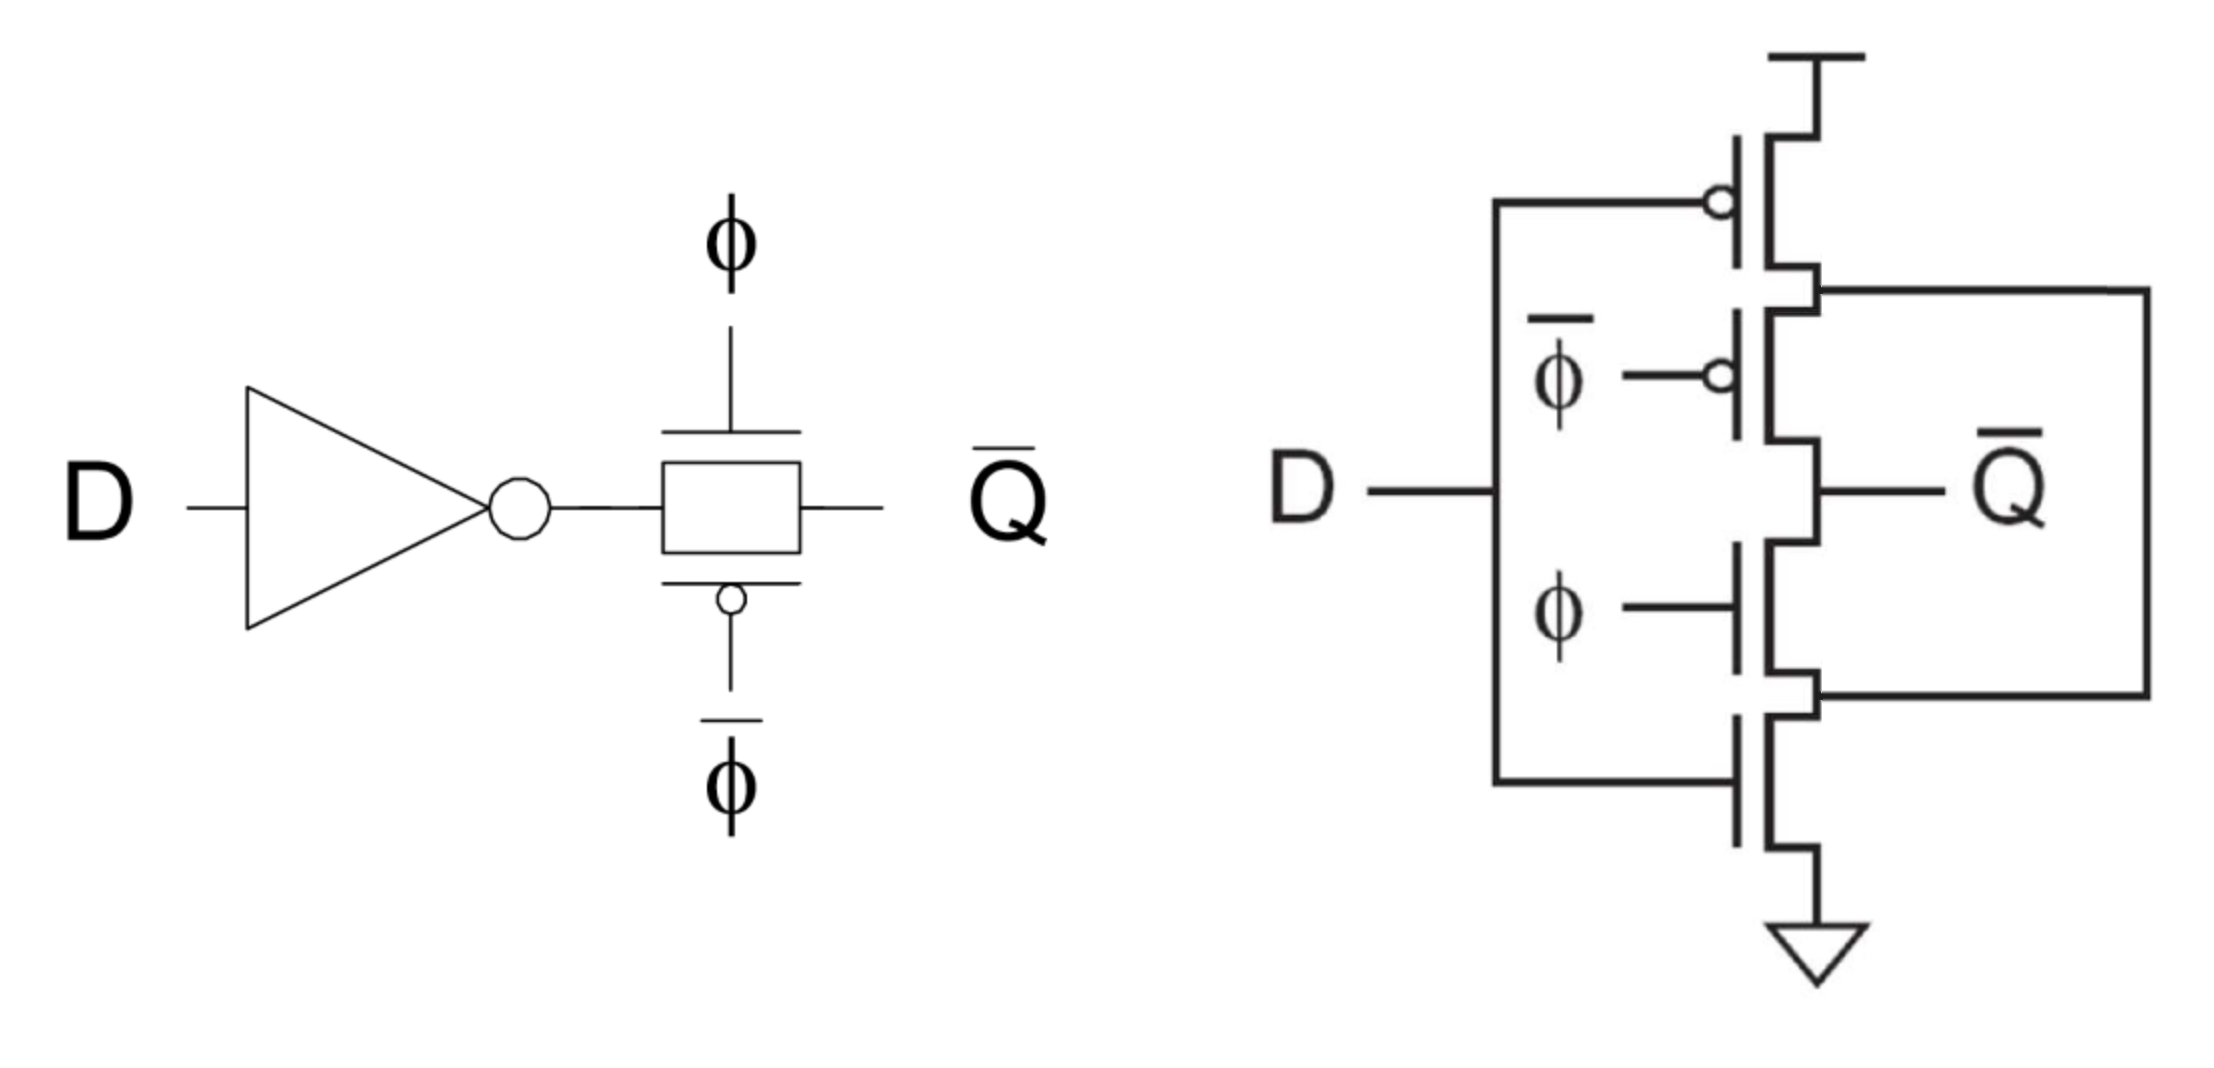
\includegraphics[width=80mm]{TransmissionGate.png}
\caption{Transmission Gate}
\label{C2MOS}
\end{figure}

It should also be noted that an inverter connected to a transmission gate, can be replaced by a C2MOS latch. If you spread the circuit out, you can see that circuit is equivalent except that the intermediate nodes between the clocked transistors and the inverter transistors are connected. 

The C2MOS latch takes less area, but the transmission gate version is faster. This is because the clocked transmission gate acts like two resistors in parallel that the the logic needs to be transferred across, whereas with the C2MOS, the logic has to be transferred across only one resistor in series. 

\subsection{Flip-Flops}

A flip-flop is a pair of back-to-back latches with transmission gates with opposite logic. 

It's edge triggered because although the first latch is level triggered, since the transmission gates are opposite, the data is stuck at the first latch until the clock switches. When the clock switches, it can pass through the second transmission gate, so it only passes through on a clock edge. 

The feedback inverters are also triggered on opposite clocks. When $\phi=0$, the first transmission gate is turned on, and the feedback inverter is disabled, so the node $X$ is updated with the driven input. 


\begin{figure}[ht!]
\centering
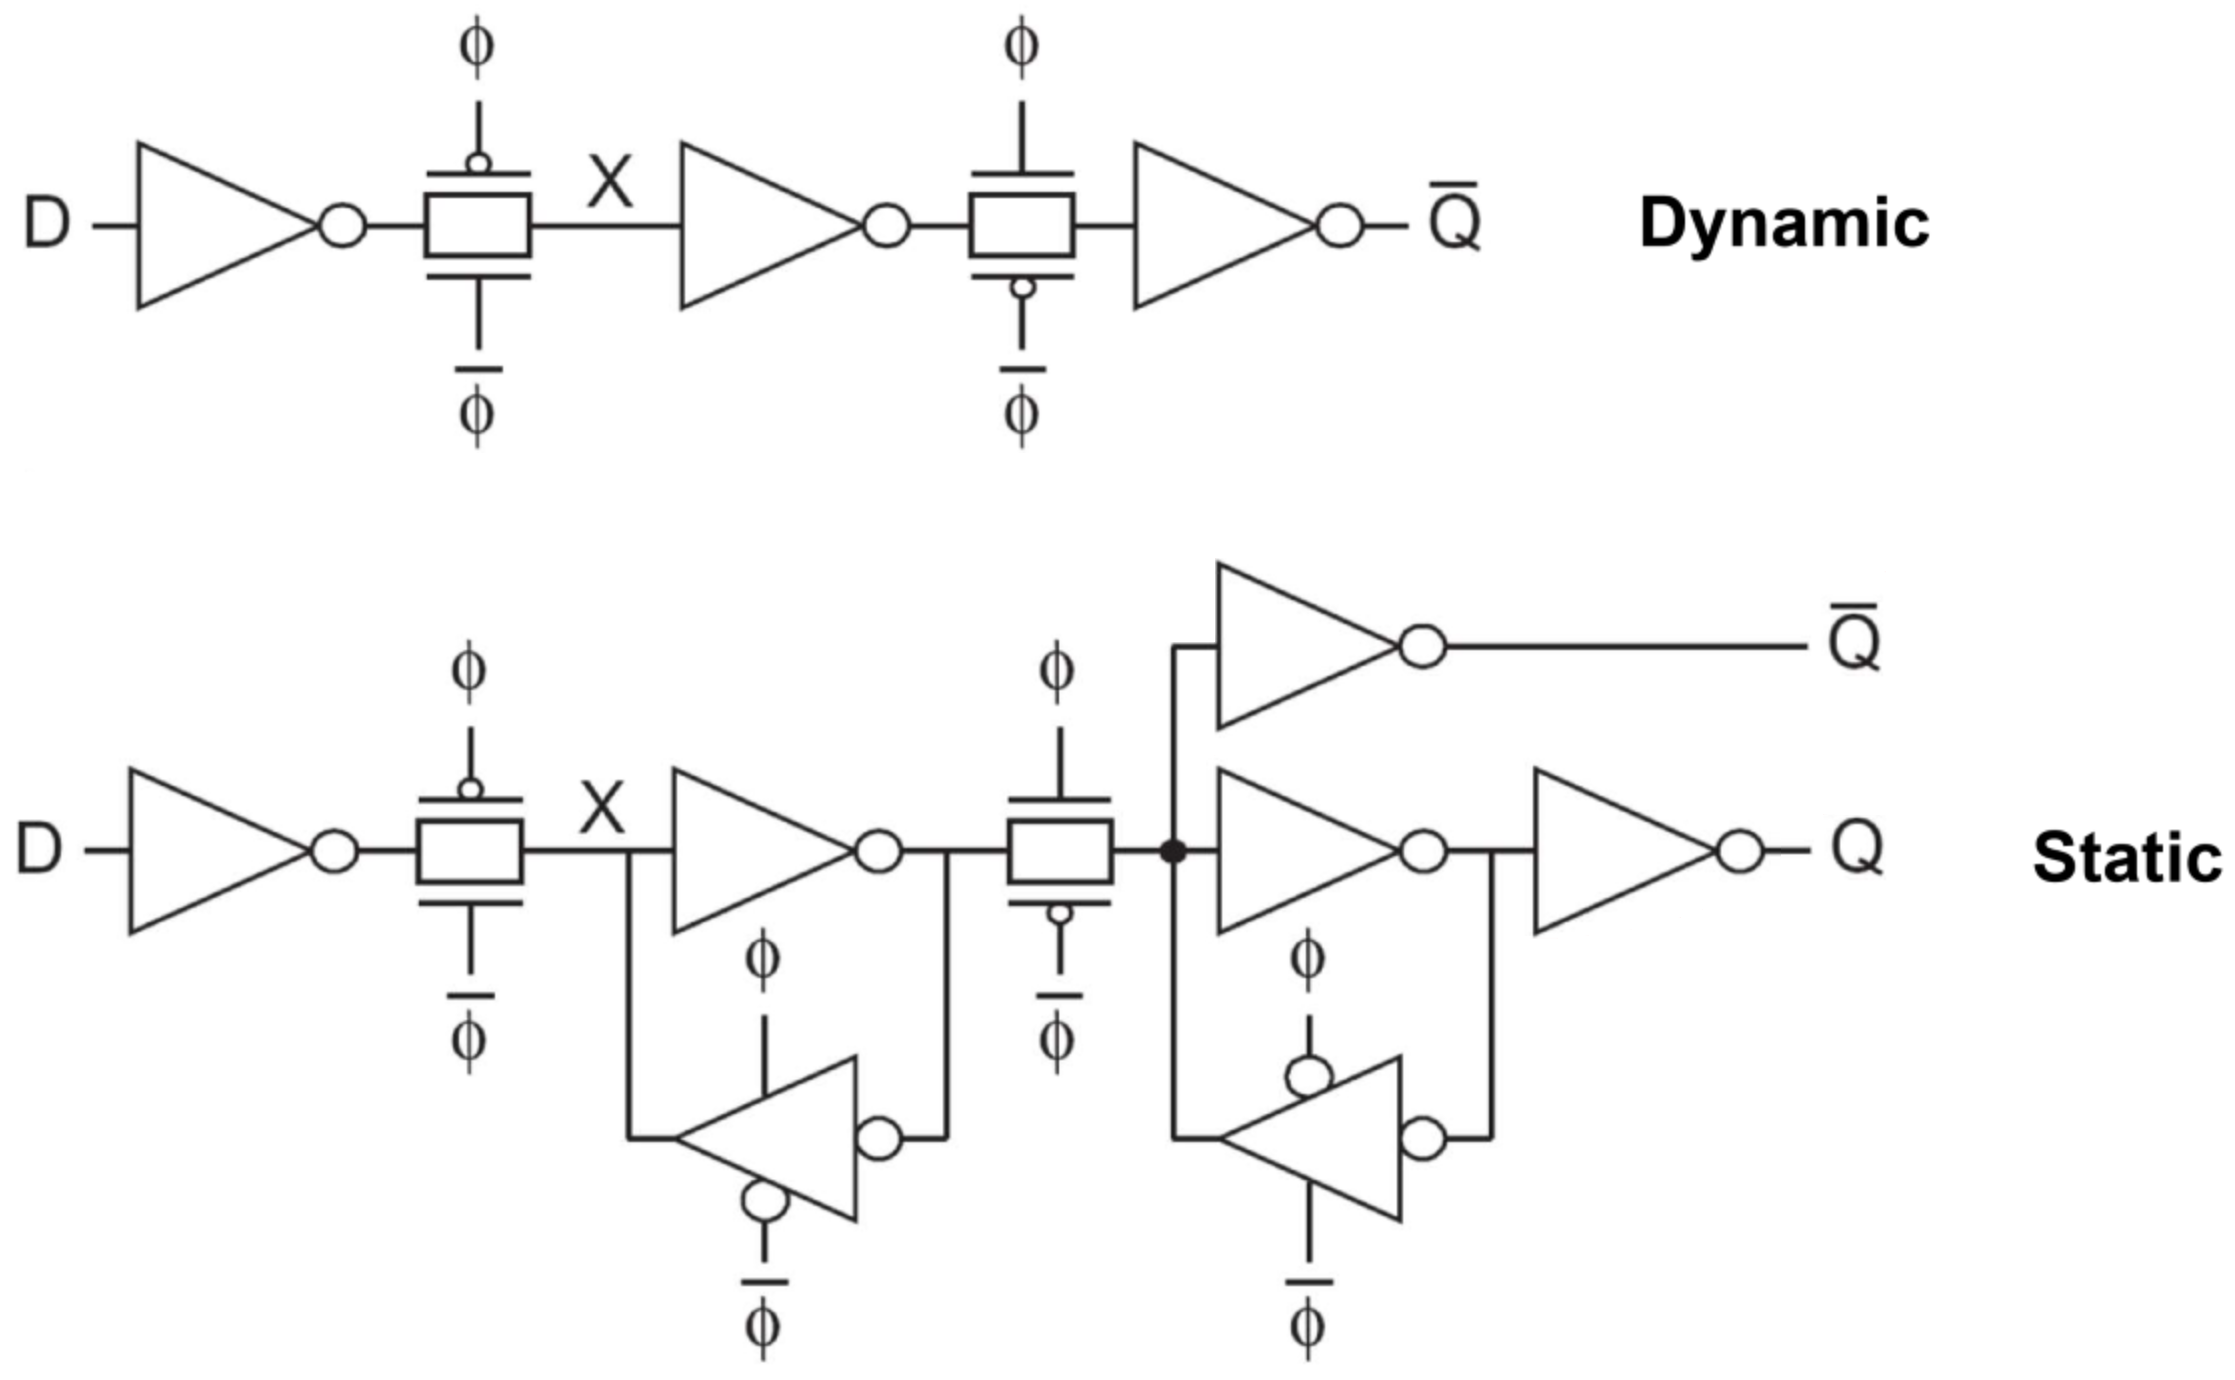
\includegraphics[width=110mm]{FF.png}
\caption{Dynamic and Static Flip-Flops}
\label{C2MOS}
\end{figure}

When $\phi=1$, the first transmission gate is turned off and the first feedback is enabled, storing the value at X. Meanwhile, the second transmission gate is turned on and the feedback inverter is turned off, allowing the output to be updated from $X$. 

This flip-flop also has buffered outputs to prevent backdriving, and an input buffer to prevent a diffusion input.

\subsubsection{Reset}

The reset forces the output to go low when asserted. With a an asynchronous reset this will happen immediately, with an synchronous reset this will only happen at the clock-edge. 

\begin{figure}[ht!]
\centering
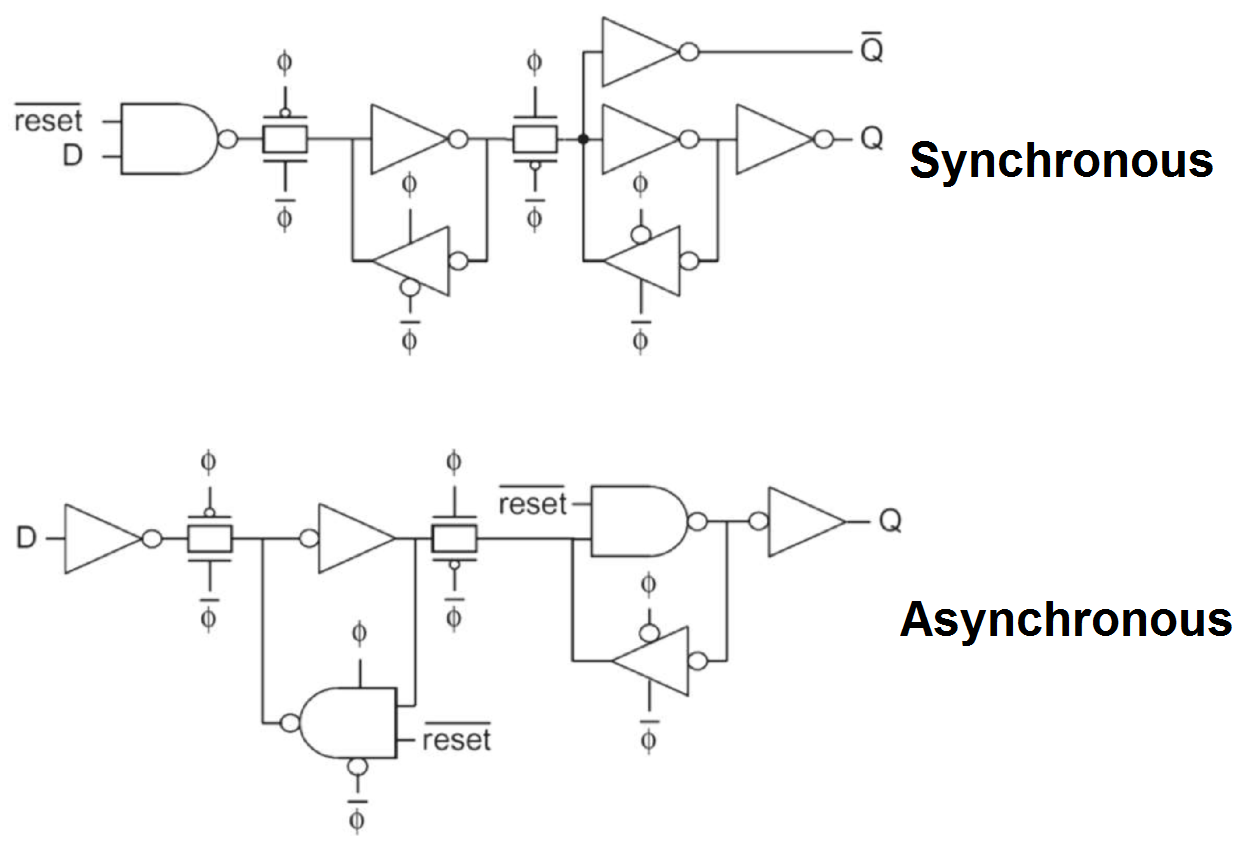
\includegraphics[width=100mm]{Reset.png}
\caption{Synchronous/Asynchronous Reset Flip-Flops}
\end{figure}

To have a set bit instead, which forces output high when asserted, use a NOR instead of a NAND.

\subsubsection{Enable}

The enable bit signals to the flip-flop to ignore the clock when low. This can be implemented in two ways. One of which is to use multiplexer that ignores the D input and feedbacks the previous output to retain its old value. This increases delay between input and output (D-Q delay) and takes up area. 

\begin{figure}[ht!]
\centering
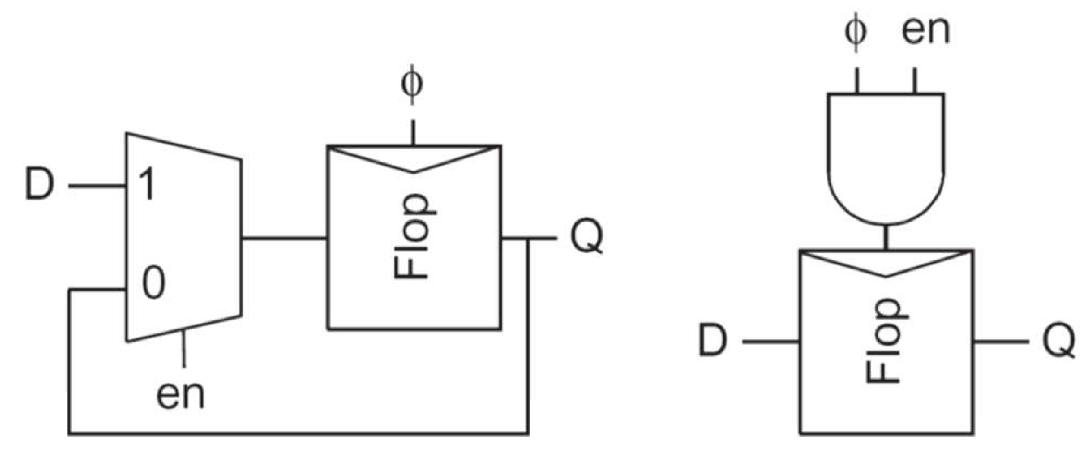
\includegraphics[width=100mm]{Enable.png}
\caption{Mux/Clock-gating Enabled Flip-Flops}
\end{figure}

The other way is to use clock-gating, that is, run the clock through an AND gate with the enable bit. This way, the flip-flop only gets a clock edge telling it to take in the new value when the enable bit is set, otherwise the clock is constant. This creates a clock-skew, where different parts of the circuit may have clock-edges triggered at different times. 


A bonus of clock-gating is that it reduces power consumption, since you won't be toggling nodes unnecessarily your activity factor will go down.

\subsection{Timing Definitions}

\begin{enumerate}

\item \textbf{Logic contamination delay}, $\mathbf{t_{cd}}$ -- This is the amount of time it takes for the output of a combinational logic block to begin to fluctuate after the input changes. While the output is fluctuating, it is said to be contaminated.

\item \textbf{Logic propagation delay}, $\mathbf{t_{pd}}$ -- After the input to a combinational logic block changes, the output may fluctuate while it is being computed. This is the amount of time it takes for the output of a combinational logic block to change to its final result after the input changes. 

\begin{figure}[ht!]
\centering
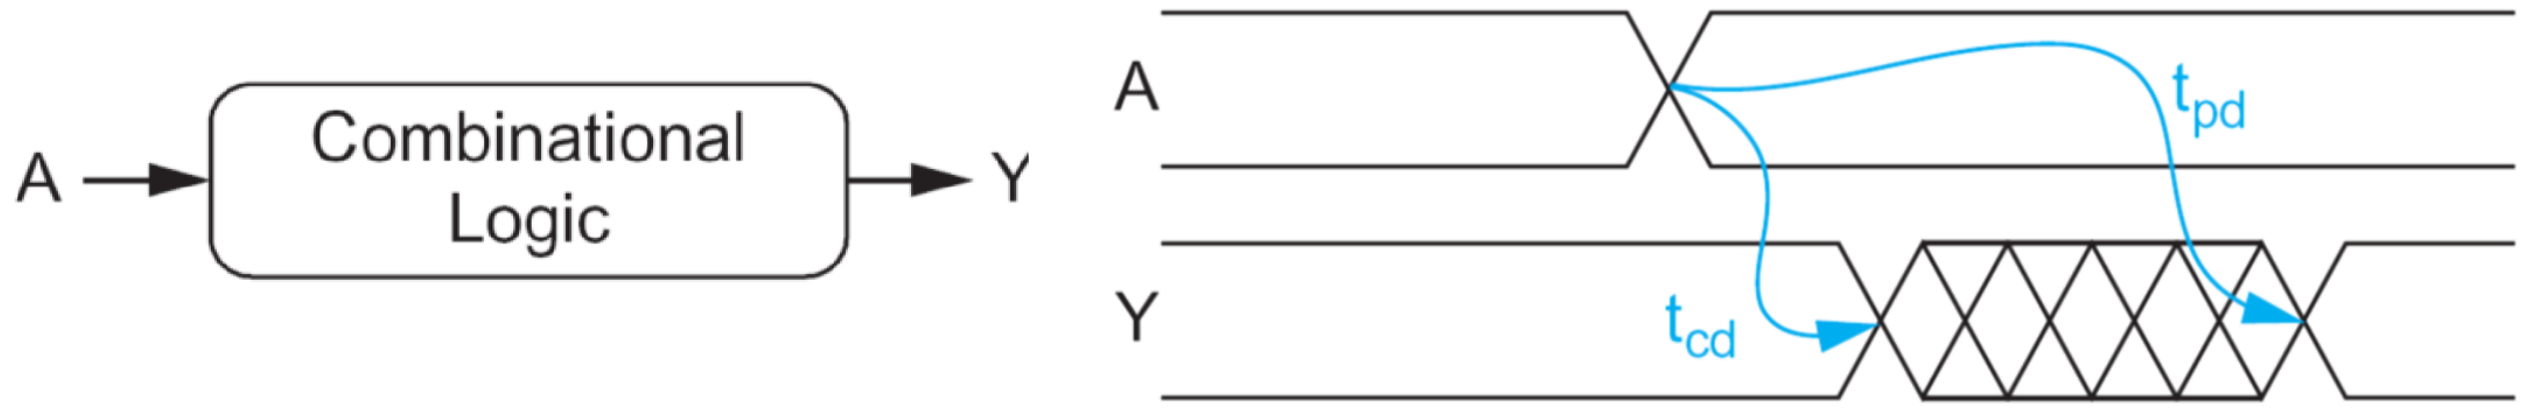
\includegraphics[width=110mm]{Prop.png}
\caption{Combinational and Propagation Delay}
\end{figure}

\item \textbf{Clock-to-Q contamination delay}, $\mathbf{t_{ccq}}$ -- This is the amount of time it takes for the output of a FF or a latch to fluctuate after the clock-edge. 

\item \textbf{Clock-to-Q propagation delay}, $\mathbf{t_{pcq}}$ -- This is the amount of time it takes for the output of the FF or a latch to change to its final result after the input changes. 

% \item \textbf{D-to-Q propagation delay}, $\mathbf{t_{pdq}}$ --
% \item \textbf{D-to-Q contamination delay}, $\mathbf{t_{cdq}}$ --
\item \textbf{Setup time}, $\mathbf{t_{setup}}$ -- This is the minimum amount of time before the clock edge that the input must be stable for the FF or latch to lock in and save the input correctly.

\item \textbf{Hold time}, $\mathbf{t_{hold}}$ -- This is the minimum amount of time after the clock edge that the input must be stable for the FF or latch to keep the value locked in correctly. This value can be negative, which implies the value can be locked in to the FF/latch before the clock edge. 

\begin{figure}[ht!]
\centering
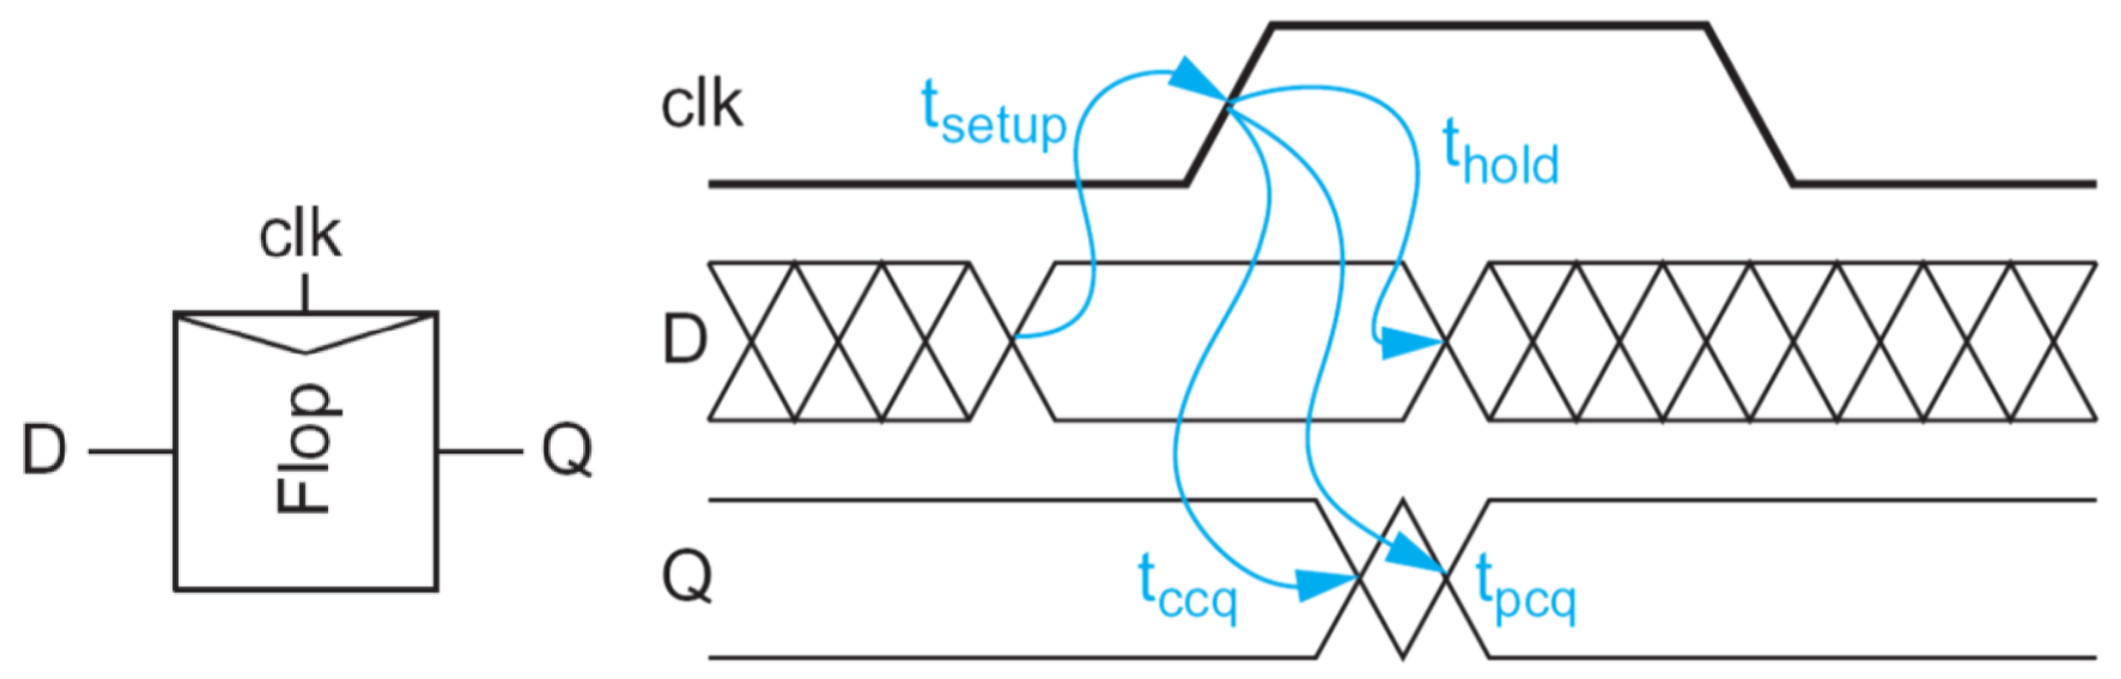
\includegraphics[width=110mm]{Setup.png}
\caption{Clock-to-Q, Setup, and Hold Times of a FF}
\end{figure}

\end{enumerate} 

Note that latches only preserve a value while in opaque mode when $\phi=0$. This means that we define the setup time and hold time of a latch with respect to its falling edge, not its rising edge. Latches also have two other propagation/contamination delays, called the D-to-Q delays, because while in transparent mode they simply propagate their input. 

\begin{figure}[ht!]
\centering
\includegraphics[width=110mm]{LatchDel.png}
\caption{Clock-to-Q, D-to-Q, Setup, and Hold Times of a Latch}
\end{figure}

\subsubsection{Setup Time (Max-Delay) Failure}

If the combinational logic takes too long and continues to fluctuate without leaving enough time to be constant for the setup time before the clock goes high, this is called a max-delay or setup time failure. In this case the FF/latch may input the wrong value. The condition to avoid this failure is as follows:

\begin{equation}
T_c \ge t_{pcq} + t_{pd} + t_{setup}
\end{equation}
\myequations{Setup Time Condition}

It can be fixed by reducing the amount of time the combinational logic takes to complete ($t_{pd}$), reducing the amount of time it takes for the computation to begin ($t_{pcq}$), or reducing the setup time ($t_{setup}$). 

\begin{figure}[ht!]
\centering
\includegraphics[width=110mm]{SetupTime.png}
\caption{Setup Time}
\end{figure}

It can also be fixed by slowing the clock frequency ($T_c$), which can be done by either increasing the power-supply or under-clocking. For this reason, although not preferable because it slows your circuit, setup time failures are not catastrophic and can be worked around.

\subsubsection{Hold Time (Min-Delay) Failure}

On the contrary to setup-time failures, hold-time failures cannot be worked around. If your circuit has hold-time violations, you will have a race condition and will not be able to fix it. Modifying the frequency and $V_{dd}$ has no influence.

If the hold-time is too large or the contamination delays are too small, then the new input to the FF will start to change before the it has had time to lock in the previous input. The condition to avoid this failure is as follows:

\begin{equation}
t_{cd} + t_{ccq} \ge t_{hold}
\end{equation}
\myequations{Hold Time Condition}


In order to make different circuits compute in parallel and arrive at another circuit simultaneously, FFs/latches should be able to be placed back-to-back without any intermediate combinational logic, where $t_{cd}$=0. 

\begin{figure}[ht!]
\centering
\includegraphics[width=110mm]{HoldTime.png}
\caption{Hold Time}
\end{figure}

\subsection{Sequencing Methods}

To execute sequential circuits, we break combinational logic into chunks and separate them with sequencing elements. There are three main ways of sequencing circuits: flip-flops, 2-phase transparent latches, and pulsed latches. 

\subsubsection{Flip-Flop Sequencing}

With flip-flops, the combinational logic between FFs must take less time than the clock period, $T_c$, in order for the value to be correctly latched in at the next clock-cycle. If the combinational logic is fast, the data should be ready at the input of the second FF, waiting for the clock to rise.

\begin{figure}[ht!]
\centering
\includegraphics[width=100mm]{Seq1.png}
\caption{Flip-Flop Sequencing}
\end{figure}

As discussed in the previous section, the timing constraints for FF-sequencing is as follows:

\begin{equation}
\begin{array}{rcl}
T_c 	 &  \ge & t_{pcq} + t_{pd} + t_{setup} \\
t_{hold} &	\le & t_{cd} + t_{ccq} \\
\end{array}
\end{equation}
\myequations{FF Sequencing Timing Constraints}

\subsubsection{2-Phase Latch Sequencing}

Recall that a FF is a back-to-back latch, triggered by $clk$ and $\overline{clk}$, which we will call $\phi_1$ and $\phi_2$. If we use a second clk that is out of phase, we can use latches and divide the full-cycle between the flip-flops into two half-cycle phases. 


The inverted clocks should have some delay between them so that they never overlap, $t_{nonoverlap}$. They should have a duty cycle of around 40\% so that between each clock being high, they are both low. 

\begin{figure}[ht!]
\centering
\includegraphics[width=100mm]{Seq2.png}
\caption{2-Phase Transparent Latch Sequencing}
\end{figure}


Because there is no overlap in the clocks and at least one clock is always low, at least one latch will always be opaque. This avoids a race condition, where the token in one stage of combinational logic can propagate through two successive sequencing elements and catch up to the token of another stage. 


2-phase transparent latching may be faster because there is one  less latch delay, and it may be possible to break your combinational logic into two stages that have less overall delay than when combined. 

However, non-overlapping clocks are not easy to make, they have a high activity factor and consume a lot of power, and have a high capacitance between them. Additionally, one of the dangers of clock-skew is that it can shift a clock such that $\phi_1$ and $\phi_2$ overlap.

The hold time is reduced by the non-overlap time. The timing constraints for 2-phase latch sequencing is as follows:

\begin{equation}
\begin{array}{rcl}
T_c 	 &  \ge & 2t_{pdq} + t_{pd1} + t_{pd2} \\
t_{hold} &	\le & t_{cd} + t_{ccq} + t_{nonoverlap} \\
\end{array}
\end{equation}
\myequations{2-Phase Latch Sequencing Timing Constraints}

\begin{figure}[ht!]
\centering
\includegraphics[width=110mm]{Nonoverlap.png}
\caption{Pulsed-Latch Sequencing Hold Time}
\end{figure}

\subsubsection{Pulsed Latch Sequencing}

Again recall that the only difference between flip-flops and latches is that latches are level-triggered. 

We can achieve the same behaviour as we get from flip-flops on a clock-edge if we change our clock to instead exhibit short high-level pulses.  This eliminates two of the latches needed in the flip-flops. 

\begin{figure}[ht!]
\centering
\includegraphics[width=100mm]{Seq3.png}
\caption{Pulsed-Latch Sequencing}
\end{figure}

The pulse time, $t_{pw}$ must be shorter than the amount of time it takes for the combinational logic to complete. If the pulse time is too long, then the combinational logic could complete and the latch would be transparent, causing a race condition as the output propagates through to the next latch. 

\subsection{Time Borrowing}

Flip-flop sequencing is not a flexible system. Data starts to move on one rising edge, and must arrive at the next FF within the setup time of the next rising edge. If the data arrives too late, the system fails. If the data arrives too early, time is wasted. This means the clock is said to have a hard-edge. 

Latch sequencing is more flexible. Data can continue to transfer through the latch while it is transparent, so the data does not need to arrive at the second latch before the rising edge. It only must arrive at the second latch within the setup time of the next falling edge. 


\begin{figure}[ht!]
\centering
\includegraphics[width=100mm]{Borrowing.png}
\caption{Time-Borrowing Latch Sequencing}
\end{figure}


This means that if the combinational logic of the first stage takes too long, then the data will not arrive at the latch before the rising edge. However, it can arrive while the clock is high and the latch will still transfer it forward. This is said to borrow time from the second stage of combinational logic, because the second stage of combinational logic must compute fast enough that it can be done between the falling edge and rising edge of one half-cycle. 

This can continue across multiple cycles, but eventually some stages need to be short enough that the time is caught up. If there is a feedback loop, there can still be time-borrowing, but it must be caught up within one cycle. The amount of nonoverlap and setup time cuts down on how much time can be borrowed. 

\begin{equation}
t_{borrow} \le \frac{T_c}{2} - t_{setup} - t_{nonoverlap}
\end{equation}
\myequations{Borrowing Time}

For an ideal latch, there is no setup and nonoverlap time and you can borrow half of the entire cycle.

\subsection{Clock Skew}

Up until now we have assumed zero clock skew. In reality clocks aren't always synchronized and arrive to different sequencing elements with some uncertainty. This decreases the maximum propagation delay, increases the minimum contamination delay, and decreases time-borrowing. 


The worst-case  scenario for the setup time is that the clock to the first element is delayed and the clock to the second element is early. This squeezes the amount of time possible for the combinational logic to complete. 

\begin{figure}[ht!]
\centering
\includegraphics[width=100mm]{WorstSetup.png}
\caption{Worst Case Scenario for Setup Time}
\end{figure}


The worst-case scenario for the hold time is that the clock to the first element arrives early and the clock to the second element is late, the opposite of the worst-case for the setup time. Since hold times issues are more severe than setup-time issues, it is better to wire the clock opposite to the direction of the logic, so later elements get the clock sooner and hold-time issues can be avoided. 

\begin{figure}[ht!]
\centering
\includegraphics[width=100mm]{WorstHold.png}
\caption{Worst Case Scenario for Hold Time}
\end{figure}



It modifies the timing equations for flip-flop sequencing like so:

\begin{equation}
\begin{array}{rcl}
T_c 	 &  \ge & t_{pcq} + t_{pd} + t_{setup} + t_{skew} \\
t_{hold} &	\le & t_{cd} + t_{ccq} - t_{skew} \\
\end{array}
\end{equation}
\myequations{Flip-flop Clock Skew Equations}

And for 2-phase latch sequencing like so:

\begin{equation}
\begin{array}{rcl}
T_c 	 &  \ge & 2t_{pdq} + t_{pd1} + t_{pd2} + t_{skew} \\
t_{hold} &	\le & t_{cd} + t_{ccq} + t_{nonoverlap} - t_{skew} \\
t_{borrow} & \le & \frac{1}{2}T_c - t_{setup} - t_{nonoverlap} - t_{skew} \\ 
\end{array}
\end{equation}
\myequations{2-Phase Latch Clock Skew Equations}

Increasing the nonovelap time helps us avoid hold-time violations, but clock skew increases the likelihood of hold-time violations. Increasing the amount of delay in combinational logic also helps us avoid hold-time violations, but eats into our setup margin so is bad for setup-time. 

\section{Volatile Memory}

Random access memory (RAM) is memory that is indexed with an address, and it has an access latency independent of the address. This contracts with serial access memory which is accessed by sequentially traversing the memory, and so the latency is dependent on the address. Another memory technology still is content-addressable memory (CAM). CAM determines which address contains the data specified by a provided key -- it is used when looking for pointers rather than data. 

The distinction between RAM and ROM is still often used, but ROM (read-only memory) is a poor definition. ROM can be written-to and can also be random-access. Usually the distinction being made is memory that needs power to preserve its data (RAM), vs memory that does not need power to preserve its data (ROM). The better definition is volatile/nonvolatile memory.

Static RAM (SRAM) is made of static cells, these are driven by $V_{dd}$ or GND feedback to retain the data. SRAM is very fast and static-circuits are very reliable, but requires 6-transistors per bit. 

Dynamic RAM (DRAM) is made of dynamic cells, using the charge of a capacitor to store the data. These only require one capacitor and a transistor, so is very dense, but deals with complexity due to the dynamic charge. Leakage from the capacitor means that the cell must by cyclically refreshed (read then re-written). They also have slower access than the SRAM. 




\subsection{Memory Array Architecture}

Regardless of the memory cell technology, most memories have a similar array architecture. Each cell  has either one bidirectional port for read/writing or separate ports if density isn't the priority. 

The row-decoder is provided with an address of $n$ bits to activate one of the $2^n$ rows by asserting the row's wordline. When a row is enabled, each cell on that row shorted to that column's bitline. 

\begin{figure}[ht!]
\centering
\includegraphics[width=60mm]{Array.png}
\caption{Memory Array}
\end{figure}

In a read operation, the memory cells write their value to the bitline, which is then read in the column circuitry. In a write-operation, the bitlines are driven with a value, which overpowers the value stored in the cells in the asserted wordline and the new value is preserved. 

Since the driving power of the memory cells may be weak, particularly in the case of DRAM, and the bitlines are long (thus capacitive) it can be challenging for the memory cell to either raise or deplete the entire bitline. So the bitlines may be preconditioned to $V_{dd}/2$. This means the memory cell only needs to slightly drag up or drag down the voltage of the bitline, which is then amplified to a 1 or 0, making the process much faster. 

To ensure a square-shape so that neither the bitlines nor the wordlines are longer than necessary, we use a folded structure, where multiple words are shared across one wordline. 

(...) Skipped section about memory hierarchy.

\subsection{SRAM}

SRAM uses a memory cell with internal feedback to retain the value while power is applied. An SRAM cell is denser than FFs or latches which also has the bonus that it has less wiring and has lower dynamic power consumption. We make these cells smaller by offsetting any additional complexity to the reading/writing mechanism.

SRAM is also compatible with standard CMOS processes, is faster and simpler to use than DRAM. It is widely used in caches, registers, tables, and scratchpads. A scratchpad is like a cache, but instead of containing a copy of data stored in memory, a scratchpad has no other copies of the data. This basic circuit, as well as the level-shifter circuit (???), have not changed in a long time.

\begin{figure}[ht!]
\centering
\includegraphics[width=40mm]{SRAM.png}
\caption{SRAM Cell}
\end{figure}

An SRAM cell uses six transistors. Four transistors act as two cross-coupled inverters. These should be strong enough for them store the bit and correct leakage and disturbances during a read or noise, but weak enough for them to be overpowered. 

Two transistors act as accesses to the output of each inverter to the $bit$ and $\overline{bit}$ lines. 

\subsubsection{SRAM Read}

To conduct a read of an SRAM cell, first precharge both bitlines high, then disconnect the driver and allow them to float. Then assert the wordline, creating a connection between the output of each inverter and the bitlines. At least on of the bitlines will be pulled down by the cell. 

\begin{figure}[ht!]
\centering
\includegraphics[width=110mm]{SRAMRead.png}
\caption{SRAM Read ($Q_o=0, \overline{Q}_o=1$)}
\label{SRAMRead}
\end{figure}

In order for the cell to be read easily, the access transistors should be smaller than the inverting transistors. Consider the case in Figure \ref{SRAMRead}. Initially $Q=0$ and  $\overline{Q}=1$. Then both $bit$ and $\overline{bit}$ are precharged to 1, and the wordline is asserted. 

The charge from the $bit$ is shared through $A_1$ and bumps up the charge at $Q$. If this bump was too high, then during our read operation, we would raise $Q$ too high and it could actually flip the value of the back-to-back inverters. 

To ensure the back-to-back inverters will correct the bump in $Q$, $D_1$ must be larger than $A_1$, so that it overpowers $A_1$ the charge from $bit$ depletes to ground faster than it can accumulate at $Q$. This is of course true for $A_2$ and $D_2$ as well. 

By having inverted bitlines, we can ensure symmetry between the two back-to-back inverters, which reinforces the positive feedback action and makes the cell more immune to crosstalk or disturbances to one line. 

\subsubsection{SRAM Write}

To conduct a write of an SRAM cell, drive $bit$ (and $\overline{bit}$) with the value you want to store (and its inverse). Then raise the wordline to turn on the access transistors. The values on the bitlines will overpower the cell and the cross-coupled inverters will lock in the value. 

Assume that initially $Q=0$ and $\overline{Q}=1$, and we want to store a 1 so $bit=1$ and $\overline{bit}=0$. Since we made $D_1$ larger than $A_1$ in order to be able to do a read without disturbing the value, that means we can't force $Q$ to go high through $A_1$ because it will deplete through $D_1$  faster than it can be charged. 

\begin{figure}[ht!]
\centering
\includegraphics[width=110mm]{SRAMWrite.png}
\caption{SRAM Write ($Q_o=0, \overline{Q}_o=1$)}
\label{SRAMWrite}
\end{figure}


So instead, we will switch the value by forcing $\overline{Q}$ low through $A_2$.  Since $\overline{Q}$ is 1, then $P_2$ is on and is keeping $\overline{Q}$ high. But if we make $A_2$ larger than $P_2$, then $\overline{Q}$ will discharge faster through $A_2$ than it will be charged through $P_2$, so the value at $\overline{Q}$ can flip to 0. Once $\overline{Q}$ goes low, $D_1$ turns off and $P_1$ turns on, pulling $Q$ high. 

\subsubsection{SRAM Sizing}

As we have seen, the bitlines must not overpower the inverters during the reads, so we accomplish this by making the pull down transistors $D_1$ and $D_2$ smaller than the access transistors $A_1$ and $A_2$. This prevents a high bitline from overpowering a low node, but if we make the pull-up transistors $P_1$ and $P_2$ smaller than the access transistors, low bitlines are able to overpower a high node. 

\begin{equation}
D < A < P
\end{equation}
\myequations{SRAM Sizing Restrictions}

\begin{figure}[ht!]
\centering
\includegraphics[width=60mm]{SRAMSize.png}
\caption{SRAM Sizing}
\label{SRAMSize}
\end{figure}

(...) Skipped sections about column read/writes.

\subsubsection{SRAM Layout}

In SRAM cells, standard design rule checks (DRC) is ignored. We want our cells to be as dense as possible, so we can use multiple metal layers, break diffusions, wire diagonally, do whatever it costs to make them small. Greater than 90nm, the standard layout is that seen in Figure \ref{SRAMLayout}. 

\begin{figure}[ht!]
\centering
\includegraphics[width=70mm]{SRAMLayout.png}
\caption{SRAM Layout ($>90nm$)}
\label{SRAMLayout}
\end{figure}

The inverters are on the middle left and right and the output of each is connected to the input of the other.The ground lines are routed in M2, the bitlines are routed top-to-bottom, and the wordline is routed in both M1 and polysilicon. The wordline crosses the green diffusion twice at the bottom, these are the two access transistors.

We can tile these SRAM cells together to share $V_{dd}$, GND, the bitlines, and the wordline, as seen in Figure \ref{SRAMTile}. By putting the diffusion contacts at the cell-boundary and mirroring the cells, we can share the diffusion across multiple cells to reduce the number of diffusion breaks/contacts, thus reducing contact capacitance by half. 

\begin{figure}[ht!]
\centering
\includegraphics[width=30mm]{SRAMTile.png}
\caption{SRAM Tile ($>90nm$)}
\label{SRAMTile}
\end{figure}

The challenge with this is that there are many bends and jumps in the polysilicon and diffusions, so these are hard to produce because the limits in lithography resolution.

Smaller than 90nm, a different layout entirely is used. The "thin cell" layout is more lithography friendly, here all M1 and polysilicon runs horizontal and all M2 and diffusion runs vertical. It has no bends in the polysilicon and diffusion, and all transistors are oriented in one direction.

\begin{figure}[ht!]
\centering
\includegraphics[width=50mm]{SRAMLayout2.png}
\caption{SRAM Layout ($\le 90nm$)}
\end{figure}

Here the black represents trench interconnects. The access transistors are the points where the bitlines cross the polysilicon on top-left and bottom-right. 



\subsection{Row Decoder}

The row decoder takes an input of $n$ bits to assert one of $2^n$ rows. A $n=2$ decoder looks like that in Figure \ref{RowDecoder1}. The AND gate is created using a NAND gate and an inverter shown in the top-right.

\begin{figure}[ht!]
\centering
\includegraphics[width=40mm]{RowDecoder.png}
\caption{CMOS Row Decoder}
\label{RowDecoder1}
\end{figure}

 Note that the sizing of the NAND2 gate is atypical. Usually we size it such that all PMOS and NMOS are 2, here we size them as 1 because A1 and A0 have to drive many of these gates, so we cheat at the input of the NAND to make them smaller in size, then we make the inverter very big. (???)
 
 To reduce how much A1 and A0 have to drive, we can also use Pseudo-NMOS logic so the inputs do not need to drive the PMOS transistors, keeping the capacitance low. It has the added bonus of using a NOR gates, so the inputs will all be in parallel in the NOR gate which keeps the capacitance even lower. 
 
 \begin{figure}[ht!]
\centering
\includegraphics[width=60mm]{RowDecoderPs.png}
\caption{Pseudo-NMOS Row Decoder}
\end{figure}

The decoder for each row has to have a height that is equal to the height of the memory cells on that row, so this has to be a very skinny/short cell. The height also must remain constant with the number of inputs ($n$).

 \begin{figure}[ht!]
\centering
\includegraphics[width=60mm]{RowDecoder2.png}
\caption{Row Decoder Layout}
\end{figure}

\subsection{Column Circuitry}

Our column circuitry needs to do bitline preconditioning, it needs to amplify the weak output from a read, and in a folded architecture it needs to multiplex the words we're interested in. 

The bitlines are preconditioned by connecting them to PMOS transistors whose gate is connected to $\overline{\phi}$. Before a read, both the bitlines are precharged when the clock is high. Then one of the bitlines is pulled down slightly, and a high-skew sense amplifer pushes this to a firm low signal on the output, speeding up the read. 

 During a write, the bitlines do not need to be precharged. The write-driver pulls down one of the bitlines which overpowers the cross-coupled inverters. 

Recall that $t_{pd} \propto \frac{C}{I}\Delta V$. There are a few things we can do to speed up our memory array.

\subsubsection{Sense Amplifiers}

A 32-Kbit SRAM has 128 rows $\times$ 256 columns ($2^7 \times 2^8 = 2^{15} = 32K$). So each bitline has 128 cells, which is a lot of capacitance which means a lot of delay. For the 128 rows, we can tile our SRAM cells to mirror each other and share diffusion contacts, so there is 64C diffusion capacitance instead of 128C. 

In order to reduce our delay, we can focus on reducing the voltage swing, $\Delta V$ necessary to detect a 0 or 1. Instead of using CMOS, we could consider using dynamic-logic because it has a lower voltage swing. Further, it doesn't have an PMOS transistors which means less capacitance. By using sense-amplifiers, we reduce the amount of voltage that needs to change to identify a 0 or 1. 

During sensing, we can also turn the wordline off to avoid the bitline swinging further than necessary and consuming extra power. 

We can sense  this small voltage swing using a sense amplifier. A differential-pair sense amplifier doesn't require a clock, but it consumes static power so isn't really used in digital applications. We use a clocked sense amplifier. Like SRAM, is one of those circuits that's simple and elegant and hasn't changed in a long time.

 \begin{figure}[ht!]
\centering
\includegraphics[width=60mm]{Sense.png}
\caption{Clocked Sense Amplifier}
\end{figure}

The clocked sense amplifier only consumes power while activated, when the sense clock is high. While the clock is low, both bitlines are precharged to $V_{dd}$, then the bitlines are driven by the SRAM cell which slightly pulls down one bitline. Since the clock is low, both isolation transistors are on and the value of $bit$ and $\overline{bit}$ are shared with $sense$ and $\overline{sense}$. 

When we want to sense, the clock goes high, so the isolation transistors cut off the circuit from the rest of the bitlines. The bottom NMOS acts as a current source and the cross-coupled inverters are turned on. These inverters use regenerative feedback to quickly detect which sense line is slightly lower, pulling that side low and the other high. The rest of the read circuitry can then read the value in memory. 

\subsubsection{Column Multiplexing}

We usually fold our array to keep it square. This way it's not long and skinny so the bitlines or wordlines are not unnecessarily long and capacitive. 

But let's say you only want to read one part of the wordline, say 16 bits out of 128 on the row. Then you need to only precharge 16 of the bitlines (and their complements) and only read the values on those 16. This requires using 16 8:1 column multiplexers.

 \begin{figure}[ht!]
\centering
\includegraphics[width=100mm]{Mux.png}
\caption{8:1 Tree Decoder Multiplexer}
\end{figure}

Let's now look at the overall structure of the SRAM structure we have been discussing in Figure \ref{SRAMOver}. Here you can see the bitline precharging PMOS transistors at the top. You can see cross-coupled inverters and connected to the bitlines through the access transistors connected to the wordline. You can see the 2:1 column multiplexer, indicating whether to transmit the left bitlines or the right bitlines to the sense-amplifier. 

 \begin{figure}[ht!]
\centering
\includegraphics[width=100mm]{SRAMOver.png}
\caption{SRAM Architecture Overview}
\label{SRAMOver}
\end{figure}


\subsection{DRAM}

Like SRAM, DRAM is also volatile. It is made up of dynamic cells, so instead of cross-coupled inverters driving each other and preventing leakage, we charge up a capacitor and pray it doesn't leak. Even if the power supply is maintained, you must keep refreshing the DRAM and you must re-write to it after we read from it. 


\begin{figure}[ht!]
\centering
\includegraphics[height=40mm]{DRAM.png}
\caption{DRAM Cell}
\end{figure}


The bonus of DRAM is that it is much smaller so we can store more information and it consumes less power, but it is slower and requires more complicated control. SRAM is also constructed using standard CMOS, whereas DRAM is constructed with special processes that have been optimized for density rather than speed. People have tried to create DRAM cells in static CMOS and they have failed miserably. 

Since the bitline in DRAM is very long and it is driven by a very small capacitor, there are very small voltage swings. This means low power consumption, but it means we need to use sensitive sense amplifiers. 

To perform a read from a DRAM cell, we precharge the bitlines to be $V_{dd}/2$, then assert the wordline. The DRAM capacitor then shares its charge with the bitline either causing a slight voltage swing on the bitline (from $V_{dd}/2$) is given by Equation \ref{Eqn:VoltageSwing}, where $C_{bit}$ is the bitline capacitance and is much larger than $C_{cell}$. 

\begin{equation}
\Delta V = \frac{V_{dd}}{2} \frac{C_{cell}}{C_{cell} + C_{bit}}
\label{Eqn:VoltageSwing}
\end{equation}
\myequations{Bitline Voltage Swing}

As a quick aside, let's talk about the two-capacitor paradox and some of the interview questions conducted at Intel. 

Say you have two capacitors, both of which are fully charged and they are separated by an open ideal switch. Then at $t=0$ the switch is closed. Say $C_1 > C_2$. Which capacitor, the larger one or the smaller one, will have a bigger change in voltage across it?


\begin{figure}[ht!]
\centering
\includegraphics[height=25mm]{Paradox.png}
\end{figure}


---

We start by determining the total amount of charge stored by both capacitors: $Q_{tot}(0^-) = C_1 V_1 + C_2 V_2$. Which has to equal the same amount of charge after the switch closes $Q_{tot}(0^+) = CV = (C_1 + C_2)V$. 

Solving for $V$, we get: $$V = \frac{C_1 V_1 + C_2 V_2}{C_1 C_2}$$. 

After the switch closes, the smaller capacitor, $C_2$, will have an increase in voltage across it. So we can determine the voltage change across it to be: $$\Delta V_2 = V - V_2 = \frac{C_1(V
_1 - V_2)}{C_1 + C_2}$$.

The larger capacitor, $C_1$, will have a decrease in voltage across it because it will share its charge with $C_2$. So the voltage across it is: $$\Delta V_1 = V_1 - V = \frac{C_2(V_1 - V_2)}{C_1 + C_2}$$.

From this we can see that the only difference is the factor $C_1$ and $C_2$, so whatever the larger capacitor will have the larger voltage swing across it.

Now here's the tricky followup question. To make the math simpler, assume that $C_1 = C_2 = C$, and that $V_2(0^-) = 0$. Conceptually the problem will be the same though.

So at $t=0^-$, the total energy will just be the energy across $C_1$, where: $$U(0^-)=\dfrac{C V_1^2}{2} = \frac{Q V_1}{2} = \frac{Q^2}{2C}$$ 

At $t=0^+$, the amount of energy across each capacitor will be the same because they have the same capacitance, so they will both have have the same formula except both with have the charge across them: $$U(0^+) = \frac{(Q/2)^2}{2C} + \frac{(Q/2)^2}{2C} = \frac{Q^2}{4C}$$ 

Now here's the question: We went from $Q^2/2C$ to $Q^2/4C$ assuming ideal capacitors. So where did half the energy go?

You can do all sorts of fancy math to show that energy radiates out from the wire, or the energy lost is the kinetic energy to move the carriers. But the practical answer here is that there is no such thing as an ideal switch. 

---

To do a write to a DRAM cell, you drive the bitline either high or low or then assert the wordline. A high voltage will be forced onto the capacitor or a low voltage will let the capacitor discharge to the bitline. Because NMOS capacitors are not great at transmitting a 1, often the wordline is driven to $V_{dd2} = V_{dd} + V_t$ to avoid a degraded voltage. 

(??? ... bitlines)

\subsection{CAM}

(... ???)

\section{Non-Volatile Memory}

Both DRAM and SRAM will lose the value stored in their cells without a power connection. The original nonvolatile memory, Mask ROM, was actually read-only. The memory of Mask ROM was hardwired in fabrication in the masking process and could not be written-to. A grid of transistors was laid down, and either the presence or absence of a transistor/contact indicated a 1 or 0. Mask ROM is making a slight comeback nowadays for security reasons, because there's nothing you can do electrically to change the stored data. 


\subsection{NOR-ROM}

Let's say I wanted a 4-word, 6-bit Mask ROM, and I want to store the hex. 4-word implies four rows are be needed, so we need a 2-bit input to the row-decoder to specify which row to assert. Since there are 6-bits we need six columns. We use a dot-diagram to represent this in memory. A dot at the intersection indicates a 1.


\begin{figure}[ht!]
\centering
\includegraphics[height=35mm]{NORROM.png}
\caption{NOR-ROM and Dot Diagram}
\end{figure}

The logic of the NOR-ROM is Pseudo-NMOS. Each bitline is connected to a permanently on but weak PMOS pullup transistor. Dots represents an NMOS transistor connected directly to GND.  The wordlines are active-high -- so when asserted the presence of a transistor will pull the bitline to ground though the NMOS faster than the PMOS can charge it. The bitline is then inverted so that the presence of a transistor indicates a 1. 

This is called NOR because it's a PMOS transistor pulling it up, and then a whole bunch of NMOS in parallel pulling it down. Since this architecture requires ground lines spanning every bitline, this constrains how densely we can pack our array, so NOR-based Flash has fallen out of style.

\subsection{NAND-ROM}

NAND-ROM works a little differently. Instead of the NMOS transistors being in parallel, they are in series, hence and AND. Also the logic is oppsite here, the absense of a transistor indicates a 1 and the presence of a transistor indicates a 0. However this doesn't change the dot-diagram. The dots still represent a 1, not the presence of a transistor. 


\begin{figure}[ht!]
\centering
\includegraphics[height=35mm]{NANDROM.png}
\caption{NAND-ROM and Dot Diagram}
\end{figure}


The other thing that's different is the wordlines are active-low, so they are inverted from the row-decoder. This means that in normal operation, all the NMOS transistors are on and overpowering the pull-up PMOS transistor to pull the bitline to ground. When a wordline is asserted by  the row decoder, if there is a transistor on that row then the wordline will go to 0, turning the transistor off. 

Then the transistor in series will break the connection to ground, allowing the bitline to be charged high. This is then inverted by the output to 0, so the presence of the transistor creates a 0. Whereas if there was not a zero, then asserting the wordline would not break the connection to ground.

Because there are so many NMOS transistors in series, the sizes of the Pseudo-NMOS PMOS transistor and the NMOS transistors must be tweaked so that even if there is an NMOS at every row in series, the NMOS transistors can still overpower the PMOS. Delay grows quadratically with the number of series transistors discharging the bitline, so you should break out NAND-ROM into 16 row banks. 

\subsection{EPROM}

The next non-volatile memory was PROM (programmable ROM), which could only be programmed once but didn't need to be programmed at the fab. Each cell had a fuse that you could blow by applying a high-voltage to differentiate between 1/0. 

After that came EPROM (erasable/programmable ROM). Here you could store charge on a floating gate (FG) and use that to turn off unwanted transistors. You would then erase the data by exposing the FG to UV, which would knock off the charge.

This was improved upon with EEPROM (electrically erasable/programmable ROM), which allowed for bits of memory to be erased without UV. Flash, which is a type of nonvolatile RAM, is a variate of EEPROM. Flash differentiates itself by erasing blocks of memory at a time instead of individual bits, making it denser and faster. 

Flash is the predominant nonvolatile memory choice. However, the most common nonvolatile memory in terms of quantity of data stored on it is magnetic tape. For cost-reasons, this is what everything uploaded to the "Cloud" is stored on. 

So how does this floating-gate transistor work, and how do we use it to store a bit? Well, we use quantum mechanics! FG transistors use tunneling of electrons. We apply a high-voltage, $\approx$20V, to the body so electrons tunnel from the gate to the body. After the gate loses these electrons it becomes positively charged! The electrons cannot tunnel back without another applied high voltage, retaining the charge. 

The voltage induced on the gate effectively reduces the $V_t$ of the transistor to the point that the transistor is always on. This indicates a logic 1. 


\begin{figure}[ht!]
\centering
\includegraphics[height=35mm]{FG.png}
\caption{Floating Gate Transistor}
\end{figure}

The reverse process is used to create a logic 0. A high-voltage is applied to the gate, forcing electrons to tunnel from the bulk to the gate. This creates a negative charge on the gate, increasing the effective $V_t$ to the point that the transistor is always off. 

Tunneling is a slow process, taking on the order of milliseconds. 

With NAND Flash, access is done block-by-block, leading to fast erase and fast writing, but slower reads. It also provides higher density and lower costs. With NOR Flash, accesses are random leading to fast random reads, but slow erases/writes. 

Technologies under active research are PRAM (phase-change RAM) at CMU, 3D Xpoint which is similar to PRAM but industry driven by Intel and Micron, and FeRAM (ferroelectric RAM). 

\section{Programmable Logic Array (PLA)}

To create a PLA, you start with an matrix of inputs and their complements fed into AND gates, called the AND plane. The output of the AND gates are then fed into a matrix of OR gates, called the OR plane. 

\begin{figure}[ht!]
\centering
\includegraphics[height=40mm]{PLA.png}
\caption{PLA of $s=a\overline{b}\overline{c}+\overline{a}b\overline{c}+\overline{a}\overline{b}c+abc$ and $c=ab+bc+ac$}
\end{figure}

By dropping contacts between the inputs and the input to the AND gates and the OR gates, PLAs can perform any combinational logic function in this sum-of-products form. Control logic is usually synthesized now instead of being constructed with PLAs. Like memory, PLAs can be represented using dot-diagrams. 

AND and OR gates are not particularly efficient in CMOS, so a better implementation of PLAs in CMOS use a NOR-NOR plane. Dynamic or Pseudo-NMOS NORs are very efficient. 

\begin{figure}[ht!]
\centering
\includegraphics[height=40mm]{NORNOR.png}
\caption{AND-OR (left) and NOR-NOR (right) PLAs}
\end{figure}


Recall from DeMorgan's Law that a NOR gate is simply an AND gate with inverted inputs (bubble-pushing). So for the AND plane, we simply swap the inputs to each AND gate to be their complement. For the OR gate, we keep everything the same but invert the output to turn the NOR back into an OR.

\begin{figure}[ht!]
\centering
\includegraphics[height=60mm]{PLASchematic.png}
\caption{PLA Schematic and Layout}
\end{figure}

PLAs are much more flexible than ROM because in ROM you have to generate all the minterms, the rows from the AND gates that are then OR'd together, even if they are not needed for the output. In PLAs, you only need to generate the minterms you need, simplifying the logic. (???). This means you don't necessarily need $2^n$ rows for $n$ inputs.


\section{Power Distribution}

Power distribution networks have various functions.

\begin{enumerate}
\item Carry current from the power supply pads to transistors
\item Maintain stable, low-noise voltage
\item Provide power for average and peak demands
\item Provide return paths for current
\item Avoid electromigration and self-heating wearout (discussed later)
\item Consume little chip area and wiring
\item Easy to lay out
\end{enumerate}

If lots of transistors are toggling, then the chip could have a very high average current, and the peak current could be significantly larger than the average current. In which case, the input voltage would decrease due to IR drop. There is also inductance in any power distribution network. If there is a surge in the current requirements of one block, this will create an $L(di/dt)$ voltage.

These voltage changes, called $V_{droop}$, will also change the frequency. We want this $V_{droop}$ to be within 10\% of $V_{dd}$. 


Solder bumps each have a small inductance of 50-100pH. To diminish this inductance, we can add more inductances in parallel and it will add like resistors in parallel, diminishing the overall inductance. The reason processors have so many pins is to minimize inductance, most of these pins are just $V_{dd}$ and GND, not a signal. 

We also need to recall that the same power supply could be driving many different logic blocks. The  current will follow the path of lowest impedance, so if one logic block has significantly more impedance than other logic blocks, the current may ignore that block. We need to ensure that all blocks have the same impedance. 

To diminish noise from the power supply, we use bypass capacitors. These are large capacitors placed between $V_{dd}$ and GND. At a fixed DC current the capacitor is open and does nothing, but high-frequency noise is leaked through the capacitors instead of the circuit. Low-frequency noise can't be dealt with. These have an added bonus, where if there is a surge of required current by the circuits, the capacitors can provide the extra charge so that extra current isn't pulled from the voltage, causing an $L(di/dt)$ voltage.

\begin{figure}[ht!]
\centering
\includegraphics[height=35mm]{Power.png}
\caption{Power Supply Network}
\end{figure}

Real capacitors have a parasitic inductance at a certain frequency though, which we call the resonant frequency. Here the capacitor starts developing an inductance and looking like an inductor. When putting capacitors on a PCB, put capacitors of different sizes and types in parallel, that way the resonant frequencies are different across the different capacitors and you cover your bases.

\section{Chip Failures}

\subsection{Variation}

\subsubsection{Process}

Threshold voltage dictates how fast transistors can turn on and off, and this depends on the placement of the dopants in the channel. The standard deviation of the dopant placement is inversely proportional to the channel area.

\subsubsection{Spatial}

Performance of the die is spatially correlated to the position on the wafer. Frequency of a ring-oscillator is a very good metric of how fast the die is, and chips on the center of the wafer have a higher frequency. This is because the masking is much more uniform in the center than it is on the outside of the wafer.

\subsubsection{Aging}

Transistors change and wear out over time. Electromigration is the phenomenon of atoms moving slowly as a function of time. When we create a DC  current, electrons and holes move but we also move the atoms. Excessive electromigration can cause the atoms at vias to move, creating open circuits. This limits the amount of DC current we can send through an interconnect. 

Electromigration is a DC effect, whereas self-heating is an AC effect. The RMS current causes electrons to vibrate, generating heat. This heats the wire, and the heat then is trapped inside the dielectric surrounding the wire, heating the wire up even more. This heat makes the wire more resistive and slower. This limits how much AC current we can send through an interconnect.

Latchup was not understood until the 1970s. Lots of chips would just fail and it was unclear why. The issue was positive feedback that created a short from $V_{dd}$ to GND. 




% ----------------------------- %
% -------- BACK MATTER -------- %
% ----------------------------- %

% -------- BIBLIOGRAPHY -------- %
\clearpage
\doublespacing
\bibliography{references}
\bibliographystyle{apacite} 
\pagebreak

% -------- APPENDIX -------- %
\appendix
\onehalfspacing
\section*{Appendix}
\addcontentsline{toc}{section}{Appendix}
\renewcommand{\thesubsection}{\Alph{subsection}}

\subsection{Questions}

\subsubsection{Convert this state transition table to a PLA}

\begin{figure}[ht!]
\centering
\includegraphics[height=40mm]{Table.png}
\end{figure}

---

\subsubsection{A chip draws 24W from a 1.2V supply. The power supply impedance is 5m$\Omega$. What is the IR drop?}

$$I = \frac{24W}{1.2V} = 20A \rightarrow IR = 20A (5m\Omega) = 100mV$$

\subsubsection{A 1.2V chip switches from an idle mode consuming 5W to a full-power mode consuming 53W. The transition takes 10 clock cycles at 1GHz. The supply inductance is 0.1nH. What is the L(di/dt) droop?}

$$di = \frac{53W}{1.2V} - \frac{5W}{1.2V} = 40A,\ \ dt = \frac{10}{1GHz} = 10ns$$

$$V_{droop} = L \frac{di}{dt} = 0.1nH \frac{40A}{10ns} = 400mV$$

Reverse-engineer a layout to a schematic

Create dot diagram and NAND/NOR ROM given words of memory

Given a schematic, determine its truth table and create AND OR plane or NOR NOR plane or Pseudo-NMOS equivalent

Sizings for other logic classes

Sequential logic timing questions


\end{document}